%%% use 10pt options with the asme2ej format
%\documentclass[10pt]{asme2ej}
\documentclass[]{interact}

\usepackage{graphicx,epsfig,color,textcomp,amssymb,amsmath,mathrsfs,cancel,bbm,ulem,physics}

\usepackage{natbib}% Citation support using natbib.sty
\bibpunct[, ]{(}{)}{;}{a}{}{,}% Citation support using natbib.sty
\renewcommand\bibfont{\fontsize{10}{12}\selectfont}% Bibliography support using natbib.sty

\newcommand{\blue}[1]{\textcolor{blue}{[#1]}}
\newcommand{\red}[1]{\textcolor{red}{[#1]}}
\newcommand{\green}[1]{\textcolor{green}{[#1]}}
%\newcommand{\citepnum}[1]{\citep{[#1]}}
%% The class has several options
%  onecolumn/twocolumn - format for one or two columns per page
%  10pt/11pt/12pt - use 10, 11, or 12 point font
%  oneside/twoside - format for oneside/twosided printing
%  final/draft - format for final/draft copy
%  cleanfoot - take out copyright info in footer leave page number
%  cleanhead - take out the conference banner on the title page
%  titlepage/notitlepage - put in titlepage or leave out titlepage
%  
%% The default is oneside, onecolumn, 10pt, final


\title{Image-based Multiscale Mechanical Analysis of Strain Amplification from a Collagen Gel to an Embedded Neuron}

\author{
\name{Victor W. L. Chan\textsuperscript{a},  William R. Tobin\textsuperscript{a}, Sijia Zhang\textsuperscript{b}, Beth A. Winkelstein\textsuperscript{b}, Victor H. Barocas\textsuperscript{c}, Mark S. Shephard\textsuperscript{a}, Catalin R. Picu\textsuperscript{a,d}\thanks{CONTACT Catalin R. Picu. Email: picuc@rpi.edu}}
\affil{\textsuperscript{a}Scientific Computational Research Center, Rensselaer Polytechnic Institute, Low Center for Industrial Innocation, CII-4011, 110 8th Street, Troy, NY 12180; \\ \textsuperscript{b}Department of Bioengineering, University of Pennsylvania, 240 Skirkanich Hall, 210 South 33rd Street, Philadelphia, PA 19104; \\ \textsuperscript{c}Department of Biomedical Engineering, University of Minnesota, 7-105 Nils Hasselmo Hall, 312 Church Street SE, Minneapolis, MN 55455; \\ \textsuperscript{d}Department of Mechanical, Aerospace and Nuclear Engineering, Rensselaer Polytechnic Institute, Jonsson Engineering Center, Rm.\ 2049, 110 8th Street, Troy, NY 12180 } }

%%%% first author
%\author{Victor W. L. Chan
%    \affiliation{
%	Scientific Computation Research Center,\\
%	Rensselaer Polytechnic Institute,\\
%	Low Center for Industrial Innovation, CII-4011,\\
%	110 8th Street,\\
%	Troy, NY 12180
%    }	
%}
%
%%%% second author
%%%% remove the following entry for single author papers
%%%% add more entries for additional authors
%\author{William R. Tobin 
%    \affiliation{ Scientific Computation Research Center,\\
%	Rensselaer Polytechnic Institute,\\
%	Low Center for Industrial Innovation, CII-4011,\\
%	110 8th Street,\\
%	Troy, NY 12180
%    }
%}
%
%%%% third author
%%%% remove the following entry for single author papers
%%%% add more entries for additional authors
%\author{Sijia Zhang
%    \affiliation{ Department of Bioengineering,\\
%        University of Pennsylvania,\\
%	240 Skirkanich Hall,\\
%        210 South 33rd Street,\\
%         Philadelphia, PA 19104
%    }
%}
%
%\author{Beth A. Winkelstein
%    \affiliation{ Department of Bioengineering,\\
%        University of Pennsylvania,\\
%	240 Skirkanich Hall,\\
%        210 South 33rd Street,\\
%         Philadelphia, PA 19104
%    }
%}
%
%\author{Victor H. Barocas
%    \affiliation{ Department of Biomedical Engineering,\\
%        University of Minnesota,\\
%	7-105 Nils Hasselmo Hall,\\
%        312 Church Street SE,\\
%        Minneapolis, MN 55455
%    }
%}
%
%\author{Mark S. Shephard
%    \affiliation{ Scientific Computation Research Center,\\
%	Rensselaer Polytechnic Institute,\\
%	Low Center for Industrial Innovation, \\
%	CII-4011, 110 8th Street,\\
%	Troy, NY 12180
%    }
%}
%
%\author{Catalin R. Picu
%       \thanks{Address all correspondence for other issues to this author.} 
%        \affiliation{Scientific Computation Research Center,\\
%	Rensselaer Polytechnic Institute,\\
%	Low Center for Industrial Innovation, \\
%	CII-4011, 110 8th Street,\\
%	Troy, NY 12180; \\
%	Department of Mechanical, Aerospace and Nuclear Engineering, \\
%	Rensselaer Polytechnic Institute, \\
%	Jonsson Engineering Center,\\
%	Rm.\ 2049, 110 8th Street, \\
%	Troy, NY 12180 \\
%	email: picuc@rpi.edu
%    }
%}



\begin{document}

\maketitle    

%%%%%%%%%%%%%%%%%%%%%%%%%%%%%%%%%%%%%%%%%%%%%%%%%%%%%%%%%%%%%%%%%%%%%%
\begin{abstract}
{\it 
Needs to be filled in.
}
\end{abstract}

%%%%%%%%%%%%%%%%%%%%%%%%%%%%%%%%%%%%%%%%%%%%%%%%%%%%%%%%%%%%%%%%%%%%%%
\section{Introduction}

In early studies of tissue mechanics (reviewed in Fung's book), the focus was on developing constitutive equations that described the mechanical behavior of a tissue as a continuous, homogeneous entity. Even the continuous tissue mechanics problem is extremely difficult, with issues such as viscoelasticity [\red{reference}], nonlinearity [\red{reference}], multiphasicity [\red{reference}], anisotropy [\red{reference}], active stress generation [\red{reference}], damage [\red{reference}], and growth and remodeling [\red{reference}] all coming into play under various circumstances. Much of the work in the previous century of biomechanics has attempted to capture these different complexities, and this is the appropriate level at which to attack many problems given the macroscopic nature of humans and the apparent continuity of the tissue when viewed on the macro scale.

More recently, however, it has been recognized that the essential unit that responds to a macroscopic load is in fact microscopic, such as a smooth-muscle in a growing aneurysm [\red{reference}], a somatosensory nerve ending [\red{reference}], a chondrocyte remodeling the surrounding tissue [\red{reference}], a cell remodeling its scaffold in an engineered blood vessel [\red{reference}], or - most relevant to the current work - a neurite being injured by excessive stretch [\red{reference}]. In each of these cases, a macroscopic/tissue-scale loading condition is transferred to the microscopic/cell-scale force field, which in turn drives the response. If we hope to understand the microscopic response to a macroscopic load, a scale-bridging strategy is clearly needed.

The constrained-mixture models [\red{Humphrey and Rajagopal (2002)}] have been extremely effective in predicting growth and remodeling at the continuum scale, but they do not account for the local cell stress that arises, treating the cells instead as a continuous component of a mixture. As such, constrained-mixture models are not designed to address the effect of local strain field variations due to the presence of a cell, as observed experimentally in fibroblast-populated collagen gels [Voytik-Harbin]. To explore the load around a cell and to predict the forces acting on a cell, one obviously must model the cell and its surroundings as discrete entities, not as a continuous mixture.

Numerous studies have now been made using what could be broadly termed a ``cell in a box" approach. Inspired by classic work in the theory of composite materials [Hashin], models are constructed of a cell surrounded by acellular material, with the domain shape normally a cube or rectangle representing a small region of the tissue.  In most cases [\red{references}], the approach employed is to place a cell of idealized shape (sphere or ellipsoid) in the center of the cube. A notable extension is the multi-cell simulations of Marquez, Genin, and Elson [\red{reference}], in which cylindrical or ellipsoidal cells were progressively added to the system, and a jump in effect was observed when the cells percolated the domain.  Another important contribution \citep{Lai:2013fp}] was the replacement of the closed-form constitutive equation with a multiscale model that allows better representation of the extracellular matrix structure.

In spite of these recent advances, there is still considerably more work to be done in pursuing a realistic representation of the cell's (or tumor's) mechanical environment under a given tissue load. Perhaps the most salient missing feature of current models is the fact that the microscopic entity is rarely spherical in shape.  A malignant tumor can have an extremely complex geometry [Cristini?], for example, and fibroblasts spread and polarize within a collagen matrix [\red{reference}]. There is a compelling need for methods that can account for the detailed microscale geometry when downscaling mechanical information.

[Do we want a paragraph here about computational demands for such models? I am not sure.] In order to accommodate the high computational demands required to incorporate the complex neuron geometry and the multi-scale nature of the surrounding collagen gel into our model, we employ the adaptive multi-scale simulation infrastructure (AMSI) \citep{Delalondre:2010kt} which is designed to simultaneously handle massively parallel simulations on multiple scales. 

Although the approach described herein is general, it is focused on the specific experimental system of dorsal root ganglion (DRG) neurons embedded in a collagen gel. This model system, which has been used extensively by the Winkelstein group [\red{reference}] and others [\red{reference}], allows detailed study of the cellular mechanisms of neuronal injury in a more controllable environment than can be achieved in vivo. As such, it has the potential to provide insight into the mechanism of neuronal injury under mechanical load, with biochemical markers of neuronal injury being quantified in response to different macroscopic strains and/or strain rates \citep{Zhang:2016ga}. This system has the further advantage that it can be imaged readily via confocal microscopy, providing a 3-D image of the neurite [\red{reference}].

Thus, our objective in this work was to develop a general modeling strategy in which (1) confocal microscopy or another three-dimensional imaging modality is used to generate a realistic representation of a complex cell geometry, (2) that geometric model, along with the surrounding extracellular matrix, is converted to a finite-element mesh, (3) a multiscale model is implemented on that mesh using a network microstructural model at each Gauss point \citep{Chandran:2007hy,Stylianopoulos:2007dp}, and (4) the solution of the mechanics problem is used to determine the distribution of stresses \red{Is it more appropriate to measure stress than strain? If so, We should still compare the cases of nonpainful and painful ligament loading} over the cell. To test the method, we applied it to images taken of the neuron-in-gel system used by Zhang et al.\ \citep{Zhang:2016ga} \red{other references?} to  mimic innervation of collagenous tissue. To summarize that system, dissociated dorsal root ganglion neurons were embedded in three-dimensional collagen I gels. \red{Sijia: anything else to say about the neuron culture?} Immunocytochemistry was performed with an antibody against the cytoskeletal protein $\beta$III-tubulin (Abcam Cambridge, MA) to label the neuronal structure.

%%%%%%%%%%%%%%%%%%%%%%%%%%%%%%%%%%%%%%%%%%%%%%%%%%%%%%%%%%%%%%%%%%%%%%
\section{Realistic Representation of Complex Cell Geometry}

A realistic representation of complex cell geometry was generated from three-dimensional (3D) voxelated data that originated from a stack of image slices. Noise in the voxelated data that results from the limited level of contrast in the imaging technique are removed using a combination of erosion/dilation, manual reassignment, small object removal, and smoothing operations which were applied using the \textit{ImageToModel} tool \citep{Klaas:2013ug, Klaas_conference, simmetrix}. Once processed, the voxelated data is converted into a discrete geometry via an initial triangulation that is based on voxel level operations where \red{Need to read references to understand how discrete geometry is created.} Quantization artifacts on the surface of the geometry due to the voxel nature of the data are removed using a smoothing algorithm that consists of three steps. The processed voxelated data was converted to a discrete geometry using a procedure that is based on the marching cube algorithm \citep{Lorensen:1987vr}, which was also applied through the \textit{ImageToModel} tool.

In this work, the input 3D voxelated data originated from a stack of confocal images of the neuron-in-gel system. Immunocytochemistry was performed with an antibody against the cytoskeletal protein $\beta$III-tubulin (Abcam Cambridge, MA) to label the neuronal structure. Z-stack Images (2-micron thick) were taken by a Zeiss LSM 510 confocal microscope (Carl Zeiss Inc., Thornwood, NY) using a 40X objective and with a resolution of 0.22 micron/pixel. \blue{Three different confocal image slices are shown below.} 

The confocal images were stacked together and converted to a 3D voxelated data set using \textit{ImageJ} \citep{Schneider:2012dw}, where each voxel has dimensions of 0.22$\mu$m $\times$ 0.22$\mu$m $\times$ 2$\mu$m. Subsequently, the discrete geometry generated from the voxelated neuron-in-gel data was enclosed in a box that represents the domain of the collagen gel, where the neuron-gel interface is perfectly bonded. A mesh of $\approx$ 80,000 tetrahedral elements was generated on the non-manifold neuron-in-gel geometry using the SimModeler tool of Simmetrix Inc. \citep{simmetrix,Shephard:2000vc}. The neuron-in-gel voxelated data, discrete geometry, and corresponding mesh are shown in Figs.\ \ref{fig:image_to_model}(a) - (c), respectively. 
%
% (a) Schematic of image stack - images from N2P30/Neuron/sample2 folder. 
% (b) Neuron-in-gel model. Image generated by simModeler.
% (c) Neuron-in-gel mesh. Image generated by Paraview. N2P178/3-Neuron_FT
\begin{figure}[ht]
\begin{center}
$
\begin{array}{ccc}
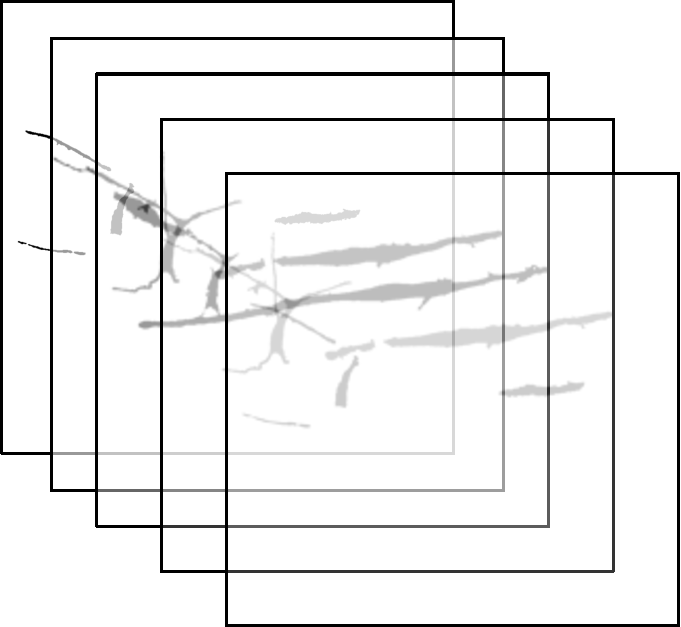
\includegraphics[height=3.5cm]{figure/ImageStack.pdf} & 
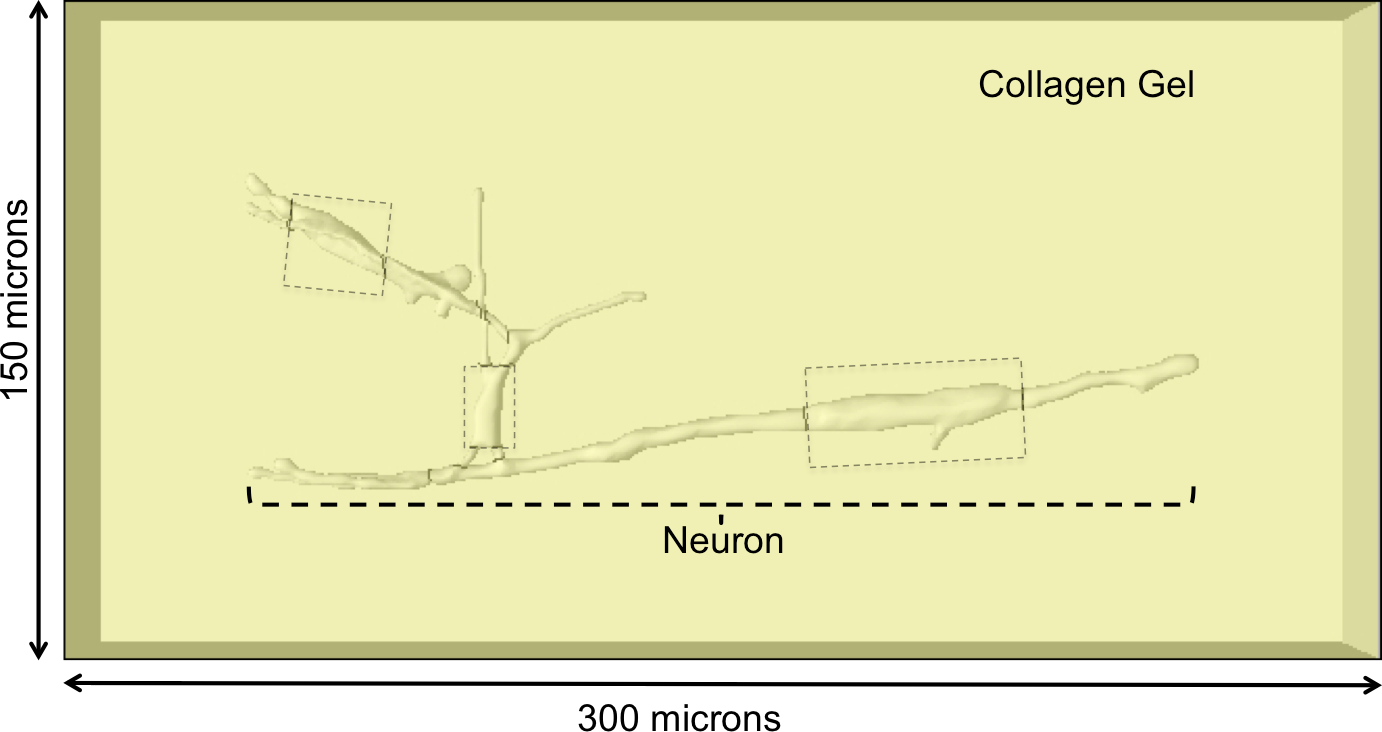
\includegraphics[height=3.5cm]{figure/neuron-in-gel_labels.pdf} &
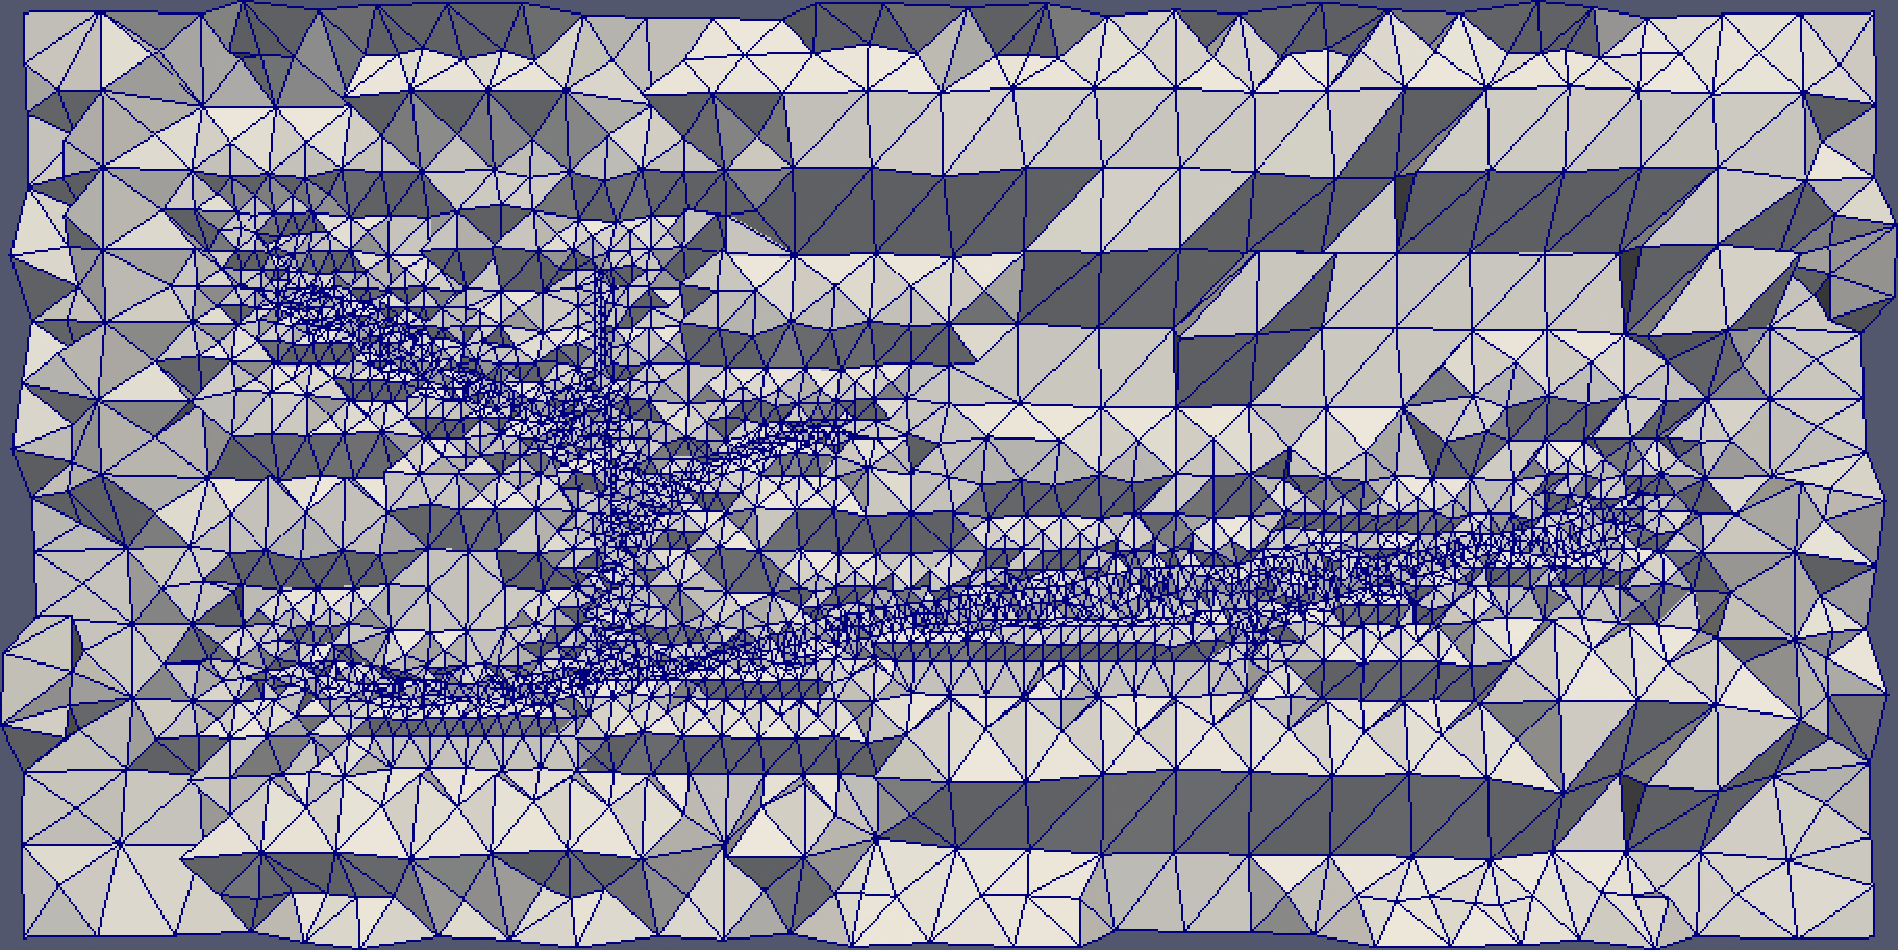
\includegraphics[height=3.5cm]{figure/neuron-in-gel_mesh.pdf} \\
(a) & (b) & (c)
\end{array}
$
\end{center}
\caption{\label{fig:image_to_model} \red{Show voxelated and discrete geometry of neuron (no gel)} (a) Stack of confocal images of a neuron structure from neuronal culture. (b) Model of neuron structure embedded in collagen gel that is generated using the \textit{ImageToModel} tool \citep{Klaas:2013ug, Klaas_conference, simmetrix} from Simmetrix Inc. The neuron structure consists of three neurons and the three cell bodies within the neuron structure are labeled with their axial length - axons are unlabeled. The region enclosing the neuron structure is the collagen gel. (c) Cut in neuron-in-gel model showing the mesh generated using the SimModeler tool \citep{simmetrix,Shephard:2000vc} from Simmetrix Inc. A mesh of $\sim$80k tetrahedral elements is used for simulations in this work.}
\end{figure}
%

%%%%%%%%%%%%%%%%%%%%%%%%%%%%%%%%%%%%%%%%%%%%%%%%%%%%%%%%%%%%%%%%%%%%%%
\section{Multi-Scale Method for Modeling Collagen Gel}
\label{sec:multiscale_method}
Collagen gels have been modeled in the past using a multi-scale formulation based on volume averaging of fiber-network representative volume elements (RVEs) \citep{Chandran:2007hy,Stylianopoulos:2007dp,Barocas:2007gk,Lai:2012ji,Lake:2012jm}, which was also employed here to model the collagen gel surrounding the neurons. The multi-scale formulation consists of two scales: the microscopic scale that represents the fiber level and the macroscopic scale that represents the tissue level. Quantities corresponding to the microscopic and macroscopic scales are denoted with $(m)$ and $(M)$ superscripts, respectively. The Einstein summation convention is applied only to subscripts $i$, $j$, and $k$.

The microscopic scale is represented by a fiber network, which defines the RVE. Each RVE is generated from the Delaunay triangulation of randomly placed seed points - the edges of the triangulation represent the fibers of the network. Each fiber only carries an axial load with the axial force given by: 
%
\begin{equation}
T^{(m)} =
\begin{cases}
\frac{E_f A_f}{B} \left[ \exp(0.5 B(\lambda_f^2 - 1)) - 1\right] & \text{if } \lambda_C \le \lambda_f \le \lambda_S \\
H_C  \lambda_f + h_C & \text{if } \lambda_f < \lambda_C \\
H_S \lambda_f + h_S & \text{if } \lambda_f > \lambda_S
\end{cases}
\label{eq:fiber_force}
\end{equation}
%
where 
%
\begin{align*}
&E_f: \text{linear modulus of a collagen fiber.} \\
&A_f: \text{cross-sectional area of fiber.} \\
&B: \text{constant parameter that controls nonlinearity.} \\
&\lambda_f \equiv \frac{l}{l_0} \text{ where } l \text{ and } l_0 \text{ are the current and initial lengths, respectively, of the fiber. } \\
&\lambda_S: \text{ fiber stretch value at which the fiber relation transitions from nonlinear to linear.} \\
&\lambda_C: \text{ fiber compression value at which the fiber relationship transitions from nonlinear to linear.} \\
&H_n \equiv E_f A_f\lambda_n \exp(0.5B(\lambda_n^2 - 1)) \text{ for } n=S \text{ or } C.\nonumber\\
&h_n \equiv \frac{E_f A_f}{B}\left[\exp(0.5 B (\lambda_n^2-1))-1\right] -H_n \lambda_n \text{ for } n=S \text{ or } C. 
\end{align*}
%
The fiber force shown in Eq.\ \eqref{eq:fiber_force} transitions from a nonlinear to linear relationship when the fiber is stretched beyond $\lambda_S$ or compressed below $\lambda_C$. The transition to a linear fiber force relationship for large fiber stretch in tension is consistent with experimental measurements of single fibers \citep{Eppell:2006hh,Svensson:2010fr}. In principle, fibers do not carry load in compression. Since the fibers in this model only have axial forces, the stiffness in compression was chosen to be significantly smaller than that in tension to mimic buckling.

In order to solve for network equilibrium in the RVE, displacement boundary conditions are imposed. The displacements at the corners of the RVE are dictated by the deformation state of the macroscopic scale via
%
\begin{equation}
u^{(c,m)}_i = (F^{(M)}_{ij} - \delta_{ij}) \frac{x^{(c,m)}_j}{L^{(m)}},
\label{eq:downscaling}
\end{equation}
%
where $F^{(M)}_{ij}$ is the deformation gradient tensor of the macroscopic scale, $u^{(c,m)}$ are the displacements at the corners of the RVE,  and $x^{(c,m)}/L^{(m)}$ are the coordinates at the corners of the RVE. In Eq.\ \eqref{eq:downscaling}, $x^{(c,m)}_j$ are coordinates of a dimensionless computational domain that is a cube spanning the domain defined by (-0.5,0.5) in each of the coordinate axes. The scale conversion, $1/L^{(m)}$, relates the unit lengths between the computational and physical domains. It is important to note that Eq.\ \eqref{eq:downscaling} is valid because the center of the RVE is defined at the origin of the computational domain. The boundary displacements on each node lying on the boundary of the RVE are determined via linear interpolation. 

Upon solving for network equilibrium in each RVE, the volume-averaged Cauchy stress tensor of the microscopic scale is computed from the forces acting on nodes that lie on the boundary of the RVE (bcl) \citep{Chandran:2007hy,Stylianopoulos:2007dp}
%
\begin{equation}
s_{ij}^{(m)} = \frac{1}{V^{(m)}} \sum_{\text{bcl}} x_i^{(m)} T_j^{(m)} ,
\label{eq:micro_stress_discrete}
\end{equation}
%
where $V^{(m)}$ is the current volume of the RVE, $T_j^{(m)}$ is the $j^{th}$ component of the fiber force, and $s_{ij}^{(m)}$ are elements of the microscopic stress tensor. The microscopic stress tensor is transformed to the macroscopic stress tensor by rescaling by $L^{(m)}$. This procedure is needed due to the difference in length scales between the physical macroscopic domain and the non dimensional microscopic computational domain. The macroscopic Cauchy stress tensor is determined from scaling $s_{ij}^{(m)}$ by 
%
\begin{equation}
\sigma_{ij}^{(M)} = s_{ij}^{(m)}\left(\frac{1}{L^{(m)}}\right)^2.
\label{eq:macro_stress_discrete}
\end{equation}
%
The Cauchy stress tensor obtained from the microscopic scale is used to solve the macroscopic force balance \citep{Chandran:2007hy,Stylianopoulos:2007dp}
%
\begin{equation}
\sigma_{ij,i}^{(M)} = \frac{1}{V^{(m)}} \int_{\partial V^{(m)}} \left( s_{ij}^{(m)} - \sigma_{ij}^{(M)} \right)u_{k,i}^{(m)} n_k dA^{(m)},
\label{eq:macro_stress_divergence}
\end{equation}
%
where $u_k^{(m)}$ is the displacement of the RVE boundary on the microscale and $n_k$ is the unit normal vector. The right-hand side of Eq.\ \eqref{eq:macro_stress_divergence} acts as a body force that accounts for the correlation between the inhomogeneous displacement of the RVE boundary and local inhomogeneities in the stress field�\citep{Chandran:2007hy,Stylianopoulos:2007dp}. Equation \eqref{eq:macro_stress_divergence} arises from integration of the microscopic-scale (RVE) Cauchy stress balance, $\sigma_{ij,i}^{(m)} = 0$. If the RVE did not deform, then the averaged equation would just be $\sigma^{(M)}_{ij,i}=0$. When the RVE deforms, however, and that deformation is position-dependent, then the average of the divergence of the stress ($\sigma_{ij,i}^{(m)}$) is no longer equal to the divergence of the average stress ($\sigma_{ij,i}^{(M)}$), and a correction term must be introduced, analogous to the corresponding term in the Reynolds transport theorem \red{Whitaker's book: The Method of Volume Averaging}. The right-hand side of Eq.\ \eqref{eq:macro_stress_divergence} is that correction and accounts for the correlation between RVE stress and boundary displacement.

The scaling parameter between the computational and physical domains, $L$, in Eqs.\ \eqref{eq:downscaling} and \eqref{eq:macro_stress_discrete} is required for both the downscaling and upscaling procedures. It is determined by comparing the average fiber length in the RVEs to that in reconstituted collagen type I networks \citep{Lindstrom:2013gd} with collagen concentration of 2mg/mL, the concentration used in \citep{Zhang:2016ga}. In the computational domain, fiber networks have a network density (total length of fibers/RVE volume) of 100 ($\pm$ 1) and an average fiber length of 0.26. The average fiber length in reconstituted collagen type I networks is 1.81 $\mu$m \citep{Lindstrom:2013gd}. Based on these average lengths, $L=7 \ \mu$m.

%%%%%%%%%%%%%%%%%%%%%%%%%%%%%%%%%%%%%%%%%%%%%%%%%%%%%%%%%%%%%%%%%%%%%%
\section{Constitutive Relationship for Modeling of Neurons}
Cross-linked axially-aligned microtubule bundles are a major structural feature of axons and give rise to macroscopic anisotropic mechanical behavior \citep{Peter:2012fc}. To account for such mechanical anisotropy, the axons are modeled as a transversely isotropic hyperelastic material \citep{JavierBonet:2008uxa,Bonet:1998vc}. The elements of the Cauchy stress tensor and spatial (Eulerian) elasticity tensor are expressed in terms of neo-Hookean (nh) and transversely isotropic (trns) components \citep{Bonet:1998vc}
%
\begin{equation}
\sigma_{ij} = \sigma^{\text{nh}}_{ij} + \sigma^{\text{trns}}_{ij} \ \ \text{ and } \ \ c_{ijkl} = c^{\text{nh}}_{ijkl} + c^{\text{trns}}_{ijkl},
\end{equation}
%
respectively, where 
%
\begin{align}
&\sigma^{\text{nh}}_{ij} = \frac{\mu}{J}(b_{ij} - \delta_{ij}) + \lambda(J-1)\delta_{ij} \nonumber\\
%
&\sigma^{\text{trns}}_{ij} = \frac{2\beta}{J}(a_r a_r - 1)\delta_{ij} + \frac{2}{J}[\alpha+2\beta\ln J+2\gamma(a_r a_r -1)]a_i a_j - \frac{\alpha}{J}(b_{is}a_s a_j+a_i b_{jr}a_r) \nonumber\\
%
&c^{\text{nh}}_{ijkl} = \lambda(2J-1)\delta_{ij}\delta_{kl} + \frac{2}{J}[\mu - \lambda J(2J-1)]\delta_{ik}\delta_{jl} \nonumber\\
%
&c^{\text{trns}}_{ijkl} = \frac{8\gamma}{J}a_i a_j a_k a_l + \frac{4\beta}{J}(a_i a_j \delta_{kl} + \delta_{ij}a_k a_l) - \frac{\alpha}{J}(a_i a_l b_{jk} + b_{ik}a_j a_l) - \frac{4\beta}{J}(a_r a_r - 1)\delta_{ik}\delta_{jl}.
\label{eq:trns_iso}
\end{align}
%
In Eq.\ \eqref{eq:trns_iso}, $b_{ij}$ are elements of the left Cauchy-Green strain tensor and $a_i$ is a component of the mapping of the direction of anisotropy in the undeformed state to the current state via the deformation gradient. In tensor notation, $\pmb{a} \equiv \pmb{F}\pmb{A}$, where $\pmb{A}$ is the direction of aniostropy in the undeformed state and $\pmb{F}$ is the deformation gradient tensor. $\lambda$ and $\mu$ are the Lam\'e constants that define the material properties of the isotropic component, while $\beta$, $\gamma$, and $\alpha$ are parameters that define the material properties of the anisotropic component. The parameters of Eq.\ \eqref{eq:trns_iso} can be written in terms of material constants as
%
\begin{align}
&\lambda = \frac{2\mu (\nu+n\nu^2)}{m} \ \ \ \ \ \gamma = \frac{E_A(1-\nu)}{8m} - \frac{\lambda+2\mu}{8} + \frac{\alpha}{2} - \beta \nonumber\\
%
&\alpha = \mu - G_A \ \ \ \ \ \ \ \ \ \ \ \ \ \ m = 1 - \nu - 2 n\nu^2 \nonumber\\
%
&\beta = \frac{\mu \nu^2(1-n)}{2m} \ \ \ \ \ \ \ \ n = \frac{E_A}{2\mu(1+\nu)},
\label{eq:trns_iso_constants}
\end{align}
%
where $\mu$ is the shear modulus, $G_A$ is the axial shear modulus, $\nu$ is the Poisson ratio, and $E_A$ is axial Young's modulus. In our analysis, the shear modulus is set to be isotropic such that $G_A=\mu$ and $\alpha = 0$. All the constants in Eq.\ \eqref{eq:trns_iso_constants} are set once all material constants ($\mu$, $G_A$, $\nu$, and $E_A$) are specified. 

%%%%%%%%%%%%%%%%%%%%%%%%%%%%%%%%%%%%%%%%%%%%%%%%%%%%%%%%%%%%%%%%%%%%%%
\section{Parameter Specifications}

\subsection{Multiscale Model for Collagen Gel}

The parameters for the multiscale model are listed in Table \ref{table:multiscale_parameters}.
%%%%%%%%%%%%%%%%%%%%%%%%%%%%%%%%%%%%%%%%%%%%%%%%%%%%%%%%
\begin{table}[ht]
\begin{center}
\begin{tabular}{ l c c }
\hline \hline
Parameter & Specification & Source \\
\hline 
$E_f$ & 200 kPa & Fit to experimental data. \\
$A_f$ & 82.5 $\mu$m$^2$ & Based on \cite{Dutov:2016gu} \\
$B$ & 20 & Fit to experimental data. \\
$\lambda_S$ &1.13 & Fit to experimental data. \\
$\lambda_C$ & 1.0 & Chosen to mimic buckling. \\ 
$H_S$ & 297.25 $\mu$N & From above parameters.\\
$H_C$ & 16.5$\mu$N & From above parameters. \\
$h_S$ & -322.74 $\mu$N & From above parameters. \\
$h_C$ & -15.67$\mu$N & From above parameters. \\
$L^{(m)}$ & 7 $\mu$m & Based on \cite{Lindstrom:2013gd}. See Section \ref{sec:multiscale_method}.\\ 
\hline \hline
\end{tabular}
\end{center}
\caption{Parameters for multiscale model of collagen gel.}
\label{table:multiscale_parameters}
\end{table}
%%%%%%%%%%%%%%%%%%%%%%%%%%%%%%%%%%%%%%%%%%%%%%%%%%%%%%%%
The value of $A_f$ was chosen according to Ref.\ \citenum{Dutov:2016gu} where the fiber radius of rat tail collagen I was measured to be 162 nm.  All other parameters for the fiber-force relationship in Eq.\ \eqref{eq:fiber_force} were chosen to obtain a good fit to an experimental stress-strain curve. To obtain the stress-strain responses experimentally, collagen I gels were subjected to uniaxial tensile loading at 0.5mm/s to 8mm (25$\%$ strain) using an Instron 5865 (Instron, Norwood, MA), as described in  \cite{Zhang:2016ga}. The Instron Bluehill software collected the force and displacement data at 1kHz during loading. The stress and strain data were subsequently determined from the force and displacement data by dividing by the initial cross-sectional area and length, respectively, of the sample. 


The stiffness in tension and compression in the linear fiber-force regimes are 29.7 kPa and 1.65 kPa, respectively, for the values listed in Table \ref{table:multiscale_parameters}. As mentioned above, the significantly smaller stiffness in compression relative to tension was chosen to mimic buckling of the fiber. The stress-strain curves calculated from simulation using the parameters in Table \ref{table:multiscale_parameters} and measured experimentally are shown in Fig.\ \ref{fig:multiscale_properties}(b).
%
% (a) fiber force curve from N2P177/LRT_Compression folder.
% (b) stress-strain curve from N2P178/1-NewParams_Cube/stress-strain folder.
% (c) Poisson ratio curve from N2P178/1-NewParams_Cube/poisson-ratio folder.
% (d) Alignment curve from N2P178/1-NewParams_Cube/alignment folder.
\begin{figure}[ht]
\begin{center}
$
\begin{array}{cc}
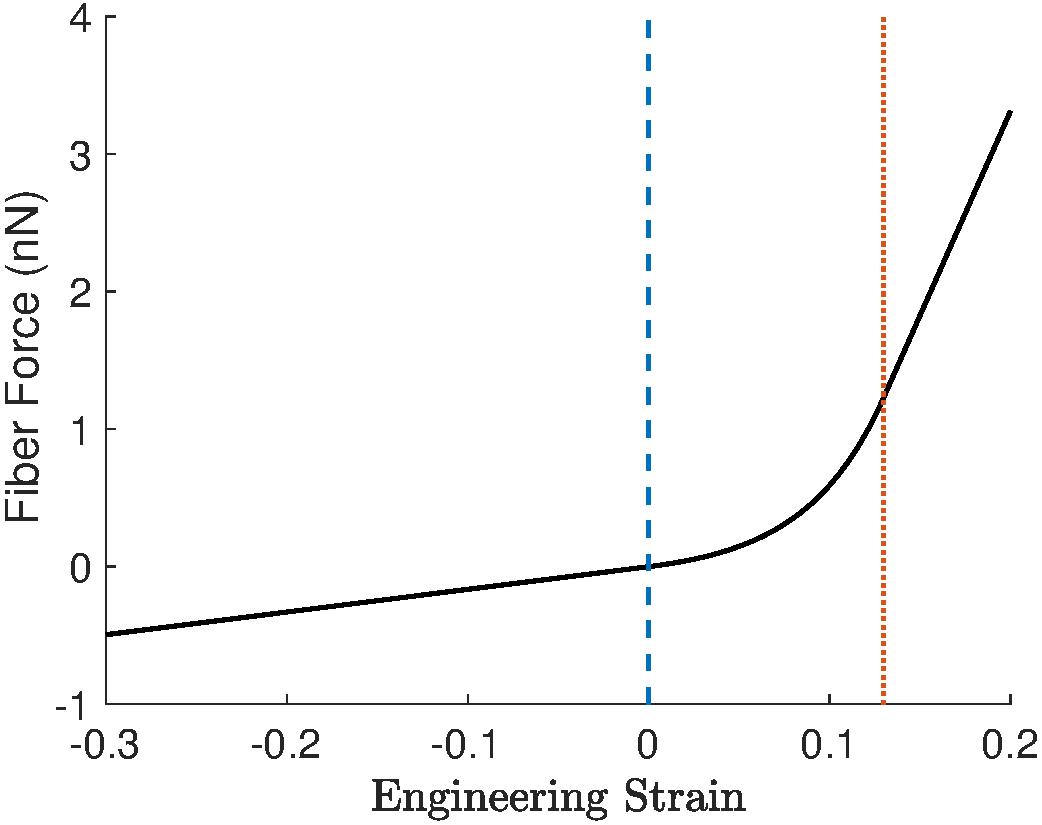
\includegraphics[height=5cm]{figure/FiberForceRelation.pdf} &
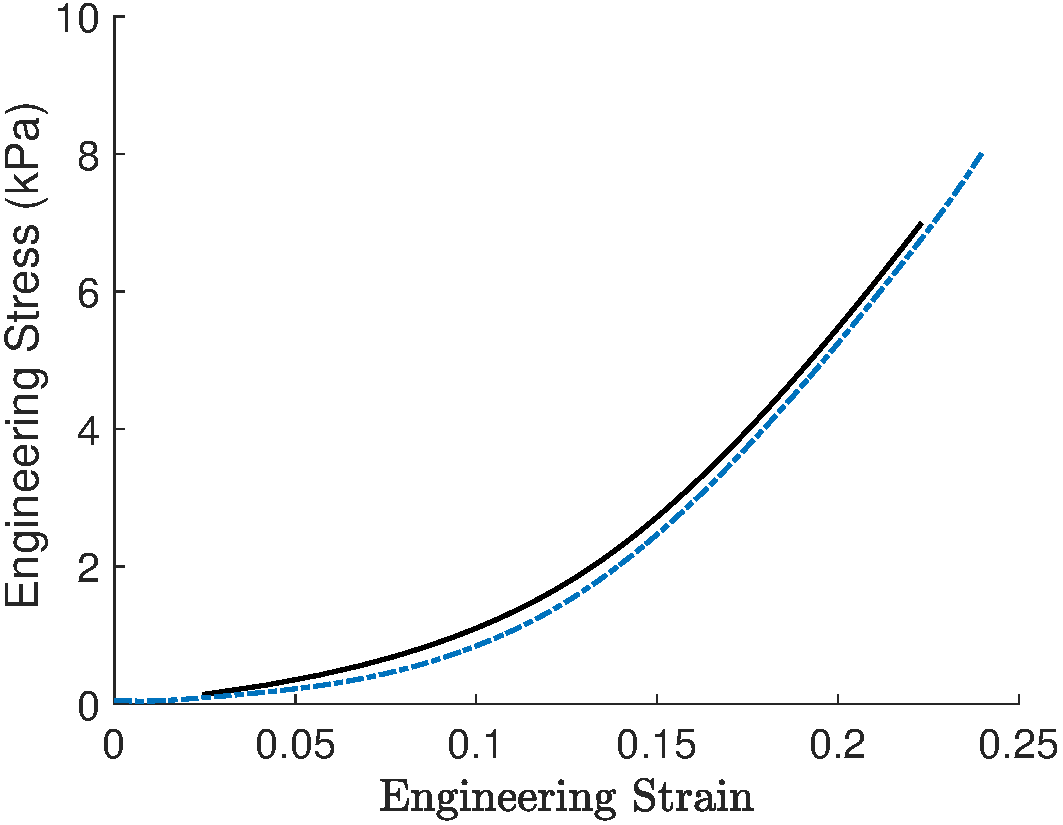
\includegraphics[height=5cm]{figure/stress_strain.pdf} \\
(a) & (b) \\
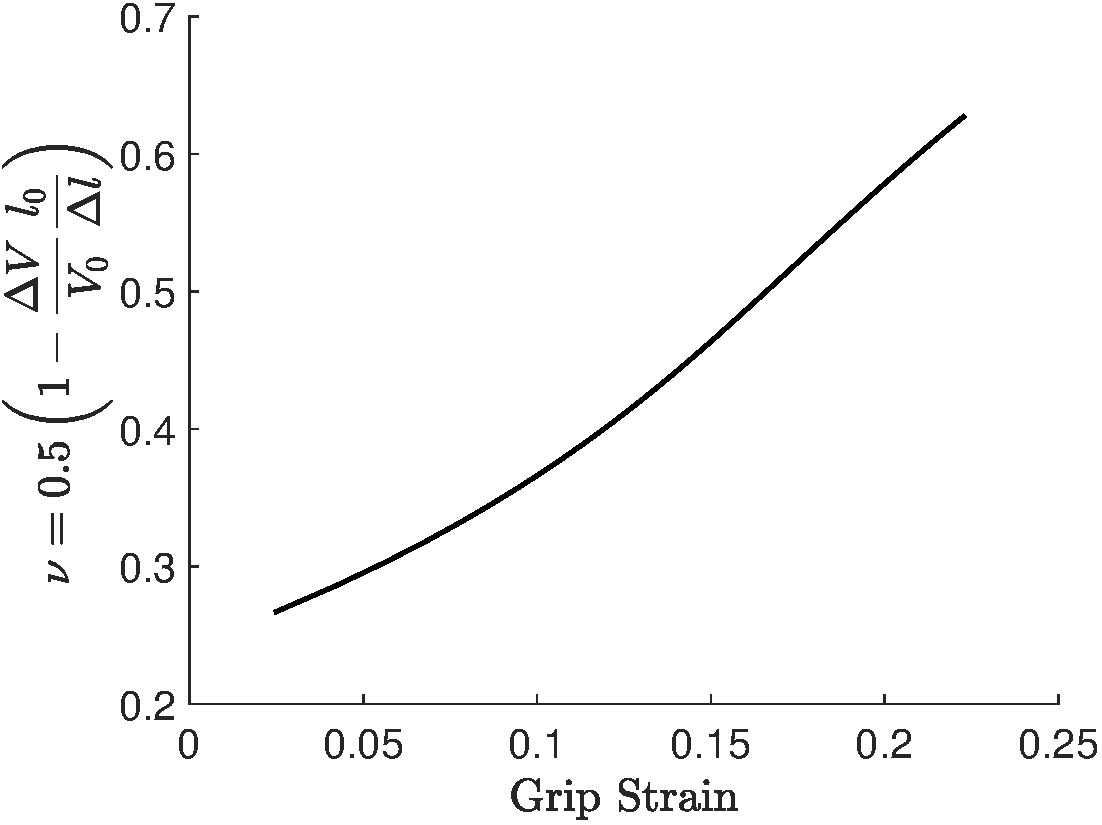
\includegraphics[height=5cm]{figure/PoissonRatio.pdf} &
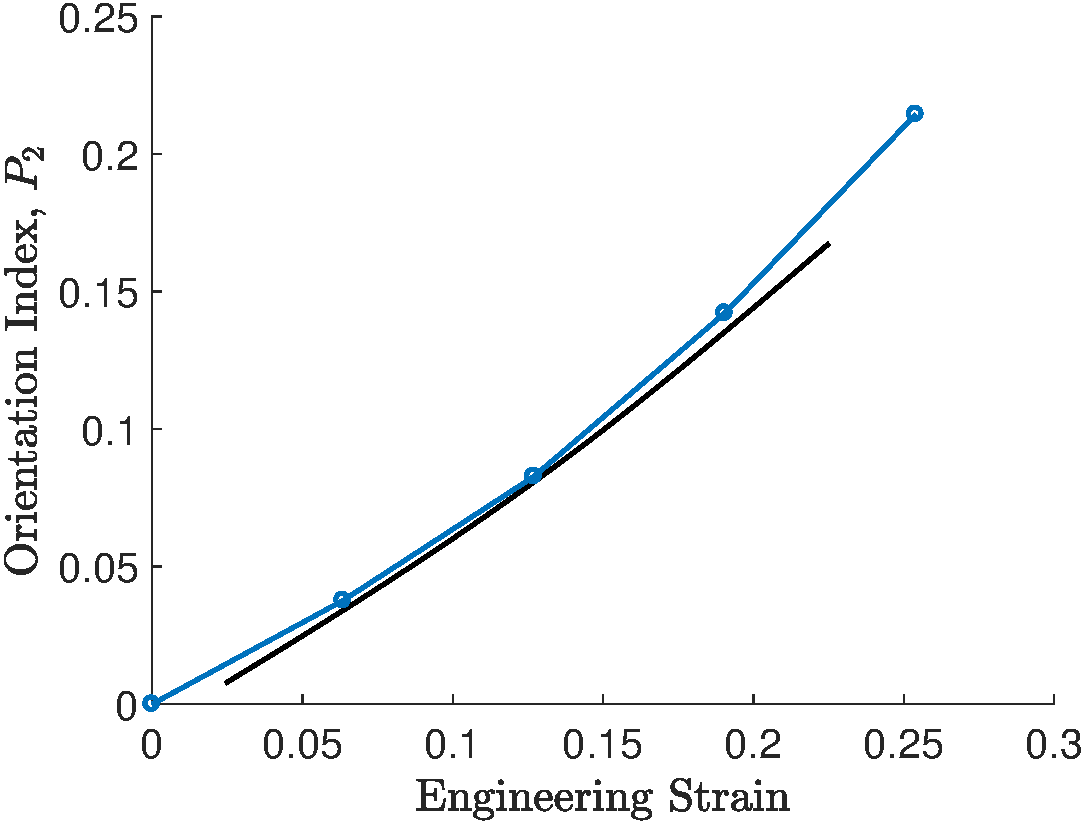
\includegraphics[height=5cm]{figure/alignment.pdf} \\ 
(c) & (d) 
\end{array}
$
\end{center}
\caption{\label{fig:multiscale_properties} \blue{Switch dotted line with solid line. Add fiber-force plot.} Plots of stress-strain curve calculated from simulation (blue ``x'') and measured experimentally (black line). The parameters of the fiber-force relationship are listed in Table \ref{table:multiscale_parameters}. Plots of (a) Poisson ratio calculated from simulation and (b) fiber alignment metric $P_2$ calculated from simulation (blue ``x") and measured experimentally (black line). Simulation results are calculated using fiber parameters listed in Table \ref{table:fiber_parameters}.}
\end{figure}
%

For the parameters in Table \ref{table:multiscale_parameters}, the Poisson ratio and fiber alignment were also examined. The Poisson ratio was determined from the volume change of the domain via
%
\begin{equation}
\nu = \frac{1}{2}\left(1- \frac{\Delta V}{V_0}\frac{l_0}{\Delta l}\right).
\label{eq:poisson-ratio}
\end{equation}
%
Equation \ref{eq:poisson-ratio} is a conventional measure of contraction that is derived from the usual definition of volumetric strain. Although Eq.\ \eqref{eq:poisson-ratio} is derived for small strain deformation, we conventionally extend the definition to the present case. The Poisson ratio as a function of the bulk strain is plotted in Fig.\ \ref{fig:multiscale_properties}(c). The Poisson ratio increases as a function of applied strain, and becomes larger than 0.5 at an applied strain of approximately $17\%$. The increasing Poisson ratio at larger applied strains is due to the presence of free volume in the network which allows significant geometric reorganization and fiber alignment \citep{Vader:2009js}. \red{At lower strains, the increasing Poisson ratio is due to the nonlinear fiber-force relationship where the stiffness in tension is increasing (see stress-strain curve in Fig.\ \ref{fig:multiscale_properties}(b)).}

Fiber alignment is measured using the orientation index $P_2$. The value of $P_2$ is calculated from the angle $\theta$ between fibers and the direction of alignment
%
\begin{equation}
P_2 = \frac{3 <\cos^2\theta> - 1}{2},
\label{eq:P2_simulation}
\end{equation}
%
where $<x>$ denotes the average of $x$ over all fibers. The value of $P_2$ ranges from 1 ($\theta=0$ or $\pi$) in which the fibers are completely aligned to -1/2 ($\theta=\pi/2$) in which the fibers are orthogonal to the alignment direction. When $P_2=0$, the fiber network is randomly oriented. The orientation index $P_2$ can be calculated from $\alpha$ and $\delta$ of the QPLI method via (see Appendix A for derivation)
%
\begin{align}
&P_2 = \frac{1}{2}\left(3 \int_0^{\pi} p(\theta) \cos^2\theta d\theta - 1\right) \nonumber\\
&p(\theta) = \frac{1}{N} \sum_{i=1}^N \left[ \frac{1-2\delta_i}{\pi} + \frac{4 \delta_i}{\pi}\cos^2(\theta - \alpha_i)\right],
\label{eq:P2_experiment}
\end{align}
%
where $\delta_i$ and $\alpha_i$ are the retardation and alignment angle, respectively, of the $i^{th}$ pixel. The fiber alignment as a function of bulk applied strain calculated from simulation and measured experimentally are plotted in Fig.\ \ref{fig:fiber_param2}(b). \red{How to explain discrepancy in alignment between simulation and experiments?}

%\textcolor{red}{[According to Professor Picu, alignment is more pronounced at low strains and less pronounced at high strains if deformation is non-affine (compared to the case of affine deformation). The behavior in Fig.\ \ref{fig:fiber_param2}(b) is in agreement if it is valid that the Delaunay fiber network that we are using deforms affinely due to the the large coordinate of the Delaunay network used in our model.]}

\subsection{Constitutive Relationship for Neuron}

The value of $E_A$ is based on the study by Peter and Mofrad \citep{Peter:2012fc}, where the mechanical behavior of axonal microtubule bundles under tension was simulated with a discrete bead-spring model. To apply their results for microtubule bundles to our neuron model, we assume that only the microtubule bundles carry force in the axon and that the stress of the microtubule bundles can be redistributed over the cross-sectional area of the axon. Since the microtubules are the stiffest component of the cytoskeleton \citep{Fletcher:2010ku}, the mechanical contribution from the actin filaments (membrane cortex) is ignored. Based on these assumptions, the axial stiffness of the axon can be related to the axial stiffness of the microtubule bundles, $E_{MTb}$, by
%
\begin{equation}
E_A = \frac{E_{MTb} A_{MTb}}{A_A},
\label{eq:EA_EMTb_relation}
\end{equation}
%
where $A_{MTb}$ and $A_A$ are the cross-sectional areas of the microtubule bundle and axon, respectively. Peter and Mofrad \citep{Peter:2012fc} suggested that the stress-strain relationship of the microtubule bundle is well represented by a power-law fit which results in an elastic modulus that is a function of strain. For this study, $E_{MTb}$ was taken to be an average value of $4\times 10^{4}$ kPa. The value of $A_{MTb}$ was determined to be 0.344 $\mu$m${}^2$ from the hexagonal bundle geometry of the microtubules (see Ref.\ \citep{Peter:2012fc} for schematic). The cross-section of the hexagonal bundle contains 19 rows of microtubules with a center-to-center microtubule spacing of 45nm. Each  individual microtubule has a diameter of 25nm. The value of $A_A$ was determined to be 19.6 $\mu$m${}^2$, which based on an average axon diameter of 5 $\mu$m in the neuron structure. From the above values, $E_A$ is determined from Eq.\ \eqref{eq:EA_EMTb_relation} to be 70 kPa. 

The parameters used in Eq.\ \eqref{eq:trns_iso_constants} for modeling the neuron structure are listed in Table \ref{table:neuron_parameters}. 
%%%%%%%%%%%%%%%%%%%%%%%%%%%%%%%%%%%%%%%%%%%%%%%%%%%%%%%%
\begin{table}[ht]
\begin{center}
\begin{tabular}{ l l }
\hline \hline
$E_A = $ 70 kPa  & axial elastic modulus calculated from Eq.\ \eqref{eq:EA_EMTb_relation}. \\ 
$E_T = $ 1.5 kPa & transverse elastic modulus. \\
$\nu = $ 0.3 & Poisson ratio. \\
$\mu = $ 0.577 kPa & shear modulus calculated from $E_T$ and $\nu$. \\ 
$G_A = \mu = $ 0.577 kPa & axial shear modulus.\\ \hline \hline
\end{tabular}
\end{center}
\caption{Parameters of Eq.\ \eqref{eq:trns_iso_constants} for modeling neuron structure. The transverse elastic modulus, $E_T$, is based on measurements of the neuron cell body by Simon et al.\ \citep{Simon:2016ig}. The shear modulus of the neuron structure is assumed to be isotropic. Therefore, $G_A = \mu = 0.577$ kPa.}
\label{table:neuron_parameters}
\end{table}
%%%%%%%%%%%%%%%%%%%%%%%%%%%%%%%%%%%%%%%%%%%%%%%%%%%%%%%%
%
The transverse stiffness of the axons and cell bodies was based on the measurements of Simon et al.\ \citep{Simon:2016ig} and chosen to be 1.5 kPa. The six constants in Eq.\ \eqref{eq:trns_iso_constants} are all determined when the values listed in Table \ref{table:neuron_parameters} are fully specified.

Lastly, the axial stiffness of the cell body was chosen based on the relative alignment of the microtubules. The microtubules transition from an aligned state in the axon to an unaligned state within the cell body \red{Sijia, Beth, Victor B.: Do you know of any reference to describe/justify this?}, where a cell-body/axon interface is defined as the starting point for the unaligned state of the microtubules. Within the cell body, the microtubules become progressively less aligned with the center of the cell body having the lease alignment. Consequently, the axial stiffness within the cell body decreases and is lowest at the center. To capture such behavior, the cell bodies are also modeled as a transversely isotropic hyperelastic material where the axial stiffness is a function of distance from the cell-body/axon interface by
%
\begin{equation}
E_A^{cell} = \left(1 - \frac{D}{t}\right)E_A.
\label{eq:cellEA}
\end{equation}
%
In Eq.\ \eqref{eq:cellEA} $D$ is the distance of an interior point of the cell body to the closest cell-body/axon interface and $t$ is a constant that dictates how quickly $E_A$ decreases when moving from the cell-body/axon interface towards the interior of the cell body. The axial stiffness decreases more quickly for smaller values of $t$.  According to Eq.\ \eqref{eq:cellEA}, $E_A^{\text{cell}}$ depends on $D$, which is the nearest distance from the cell-body/axon interface. As seen in Fig.\ \ref{fig:image_to_model}(b), the largest cell body in the neuron structure has an axial length of approximately 51 $\mu$m, which gives $D = 25.5 \ \mu$m. The axial stiffness in the neuron structure for $t=30$ and $E_A=70$ kPa is shown in Fig.\ \ref{fig:axial_stiffness}
%
%image for axial young's modulus from N2P178/3-Neuron_FT folder
\begin{figure}[ht]
\begin{center}
$
\begin{array}{c}
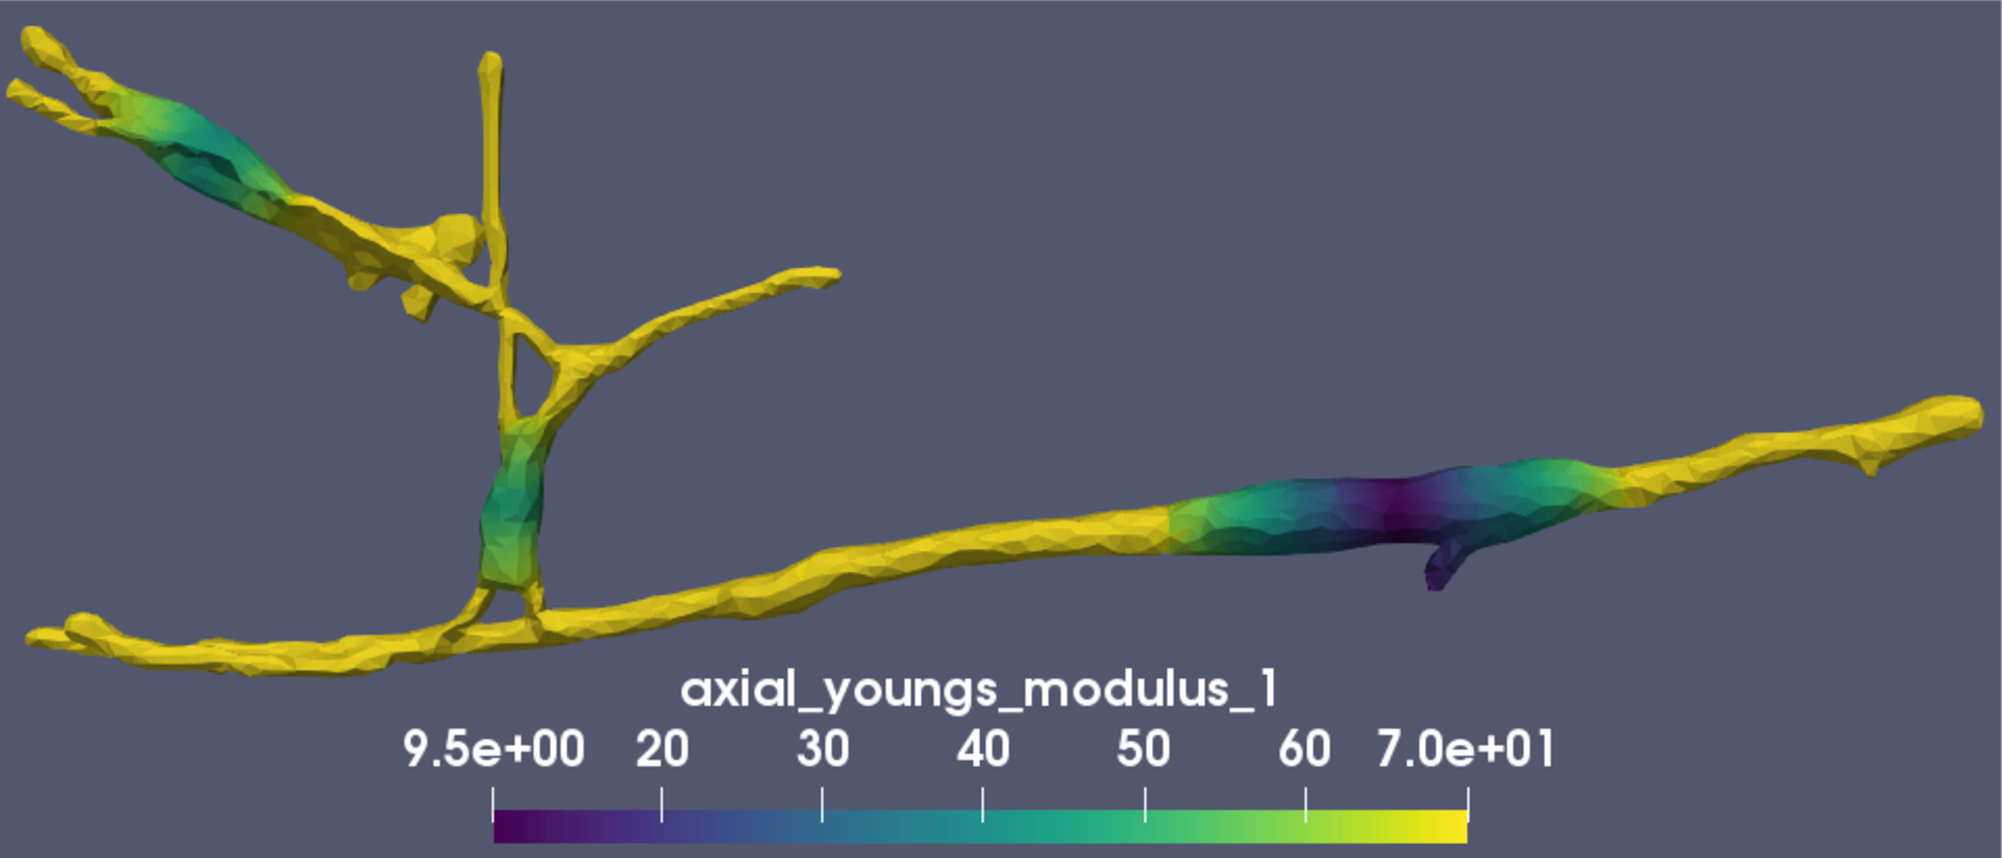
\includegraphics[height=3.5cm]{figure/axial_youngs_modulus_a30.pdf} 
\end{array}
$
\end{center}
\caption{\label{fig:axial_stiffness} Plot of axial Young's modulus for $t=30$ in Eq.\ \eqref{eq:cellEA} and $E_A=70$ kPa.}
\end{figure}
%

%%%%%%%%%%%%%%%%%%%%%%%%%%%%%%%%%%%%%%%%%%%%%%%%%%%%%%%%%%%%%%%%%%%%%%
\section{Materials and Methods}
\label{sec:materials_and_methods}
To mechanically model the neuron structure, a geometric model and its corresponding finite-element mesh is generated from confocal images of three connected neurons from a neuronal culture that was developed to mimic innervation of collagenous tissue (see Ref.\ \citenum{Zhang:2016ga} for preparation of neuronal culture). Thereby, the complex geometry of the neuron is incorporated into the simulation and enables findings from the simulation to be extended to realistic physiological environments. The collagen gel that surrounds the neuron structure is modeled using a volume-average based multi-scale technique which has been employed for the same purpose in previous studies \citep{Chandran:2007hy,Stylianopoulos:2007dp,Barocas:2007gk,Lai:2012ji,Lake:2012jm}. The embedded neuron structure is modeled using a transversely isotropic constitutive relationship to capture the anisotropic mechanical behavior of the axon \citep{Peter:2012fc}. The parameters for both models were determined from experimental measurements. An overview of the multi-scale method for the collagen gel and constitutive relationship for the neuron structure are discussed below.

%=========================================================================================================
\subsection{Generation of Model and Finite-Element Mesh from Experimental Images}
The complex geometry of a neuron is incorporated into the simulation by generating a geometric model of the neuron structure from experimentally measured confocal images. The confocal images were taken from a neuronal culture that was developed to mimic innervation of collagenous tissue. Briefly, dissociated dorsal root ganglion neurons were embedded in three-dimensional collagen I gels. Immunocytochemistry was performed with an antibody against the cytoskeletal protein $\beta$III-tubulin (Abcam Cambridge, MA) to label the neuronal structure. Z-stack Images (2-micron thick) were taken by a Zeiss LSM 510 confocal microscope (Carl Zeiss Inc., Thornwood, NY) using a 40X objective and with a resolution of 0.22 micron/pixel. The segmented stack of confocal images is shown schematically in Fig.\ \ref{fig:image_to_model}(a). 


The confocal images were stacked together and converted to a 3D voxelated data set using \textit{ImageJ} \citep{Schneider:2012dw}, where each voxel has dimensions of 0.22$\mu$m $\times$ 0.22$\mu$m $\times$ 2$\mu$m. Voxel data corresponding to different regions of the neuron structure (i.e., axon and cell bodies) were labeled with unique values. Noise arising from the limited level of contrast in the imaging technique and quantization artifacts due to the voxel nature of the data were removed using a combination of erosion/dilation, manual reassignment, small object removal, and smoothing operations which were applied using the \textit{ImageToModel} tool \citep{Klaas:2013ug, Klaas_conference, simmetrix}. The processed voxelated data was converted to a discrete geometry using a procedure that is based on the marching cube algorithm \citep{Lorensen:1987vr}, which was also applied through the \textit{ImageToModel} tool. Subsequently, the discrete geometric model of the neuron structure was enclosed in a box that represents the domain of the collagen gel, where the neuron-gel interface is perfectly bonded. The mesh of the non-manifold geometry of the embedded neuron structure was generated using the SimModeler tool of Simmetrix Inc. \citep{simmetrix,Shephard:2000vc}. The neuron-in-gel model and its corresponding mesh are shown in Figs.\ \ref{fig:image_to_model}(b) and (c), respectively. 

%=========================================================================================================
\subsection{Experimental Measurements}
The parameters for the multi-scale model of the collagen gel were chosen such that the experimental stress-strain curve is reproduced. These parameters are specified below when the formulation of the model is presented. With these parameters, the model also exhibits lateral contraction (Poisson ratio) and fiber-level alignment that are consistent with experimental measurements. An experimental stress-strain curve was measured from a rat tail collagen I gel, while fiber alignment data was measured from an innervated collagen gel (see Ref.\ \citenum{Zhang:2016ga} for preparation of the collagen and innervated collagen samples). 

To obtain the stress-strain responses experimentally, collagen I gels were subjected to uniaxial tensile loading at 0.5mm/s to 8mm (25$\%$ strain) using an Instron 5865 (Instron, Norwood, MA), as described in Ref.\ \citenum{Zhang:2016ga}. The Instron Bluehill software collected the force and displacement data at 1kHz during loading. The stress and strain data were subsequently determined from the force and displacement data by dividing by the initial cross-sectional area and length, respectively, of the sample. The fiber alignment in innervated collagenous tissue was measured using the Quantitative Polarized Light Imaging (QPLI) method \citep{Quinn:2008df,Quinn:2009bf} where alignment angle $\alpha$ and retardation $\delta$ is measured in each pixel. Our customized QPLI system \citep{Zhang:2016ga} is comprised of a fiber-optic light source (Dolan-Jenner Industries Inc., Boxborough, MA), a motor-controlled linear polarizer (Edmund Optics, Barrington, NJ) that rotates at 750 rpm, and a circular analyzer mounted to a high-speed camera (Phantom-v9.1; Vision Research Inc, Wayne, NJ) \citep{Zhang:2016ga}. The QPLI system was integrated with the mechanical testing device, and collagen I gels were placed between the rotating polarizer and the circular analyzer. Polarized light images were acquired during tensile loading at 500 fps with 14.5 pixel/mm resolution and processed using harmonic analysis to extract the alignment angle and retardation \citep{Tower:2002hk,Quinn:2008df}.

%%%%%%%%%%%%%%%%%%%%%%%%%%%%%%%%%%%%%%%%%%%%%%%%%%%%%%%%%%%%%%%%%%%%%%
\section{Implementation}
\label{sec:implementation}

%\input{figure/multi-scale-coupling-data.pdf_tex}\label{fig:coupling-data}
\subsection{Multi-scale}
Our multi-scale model is implemented using the adaptive multi-scale simulation infrastructure (AMSI) \citep{Tobin:2017ip}, which is designed to support massively parallel simulations on multiple scales. AMSI accommodates the computational demands of the multi-scale simulation by to combining existing single-scale analysis codes into multi-scale analyses.

The macroscopic simulation code and the microscopic simulation codes are independent codes coupled through the AMSI libraries. AMSI manages the parallel execution space for each code, as well as the parallel communication required for the transmission of required data between them. Each of the scales in the simulation supplies information required to inform the requirements of the multi-scale communication and the distribution of inter-scale coupling data in both the parallel execution space and the problem domain. This data is used by AMSI to communicate the coupling data required at each phase of simulation, and accommodate dynamic run-time operations such as load balancing. A discussion of the underlying design considerations of AMSI can be found in \citep{Delalondre:2010kt}.

%
\begin{figure}[ht]
\begin{center}
$
\begin{array}{c}
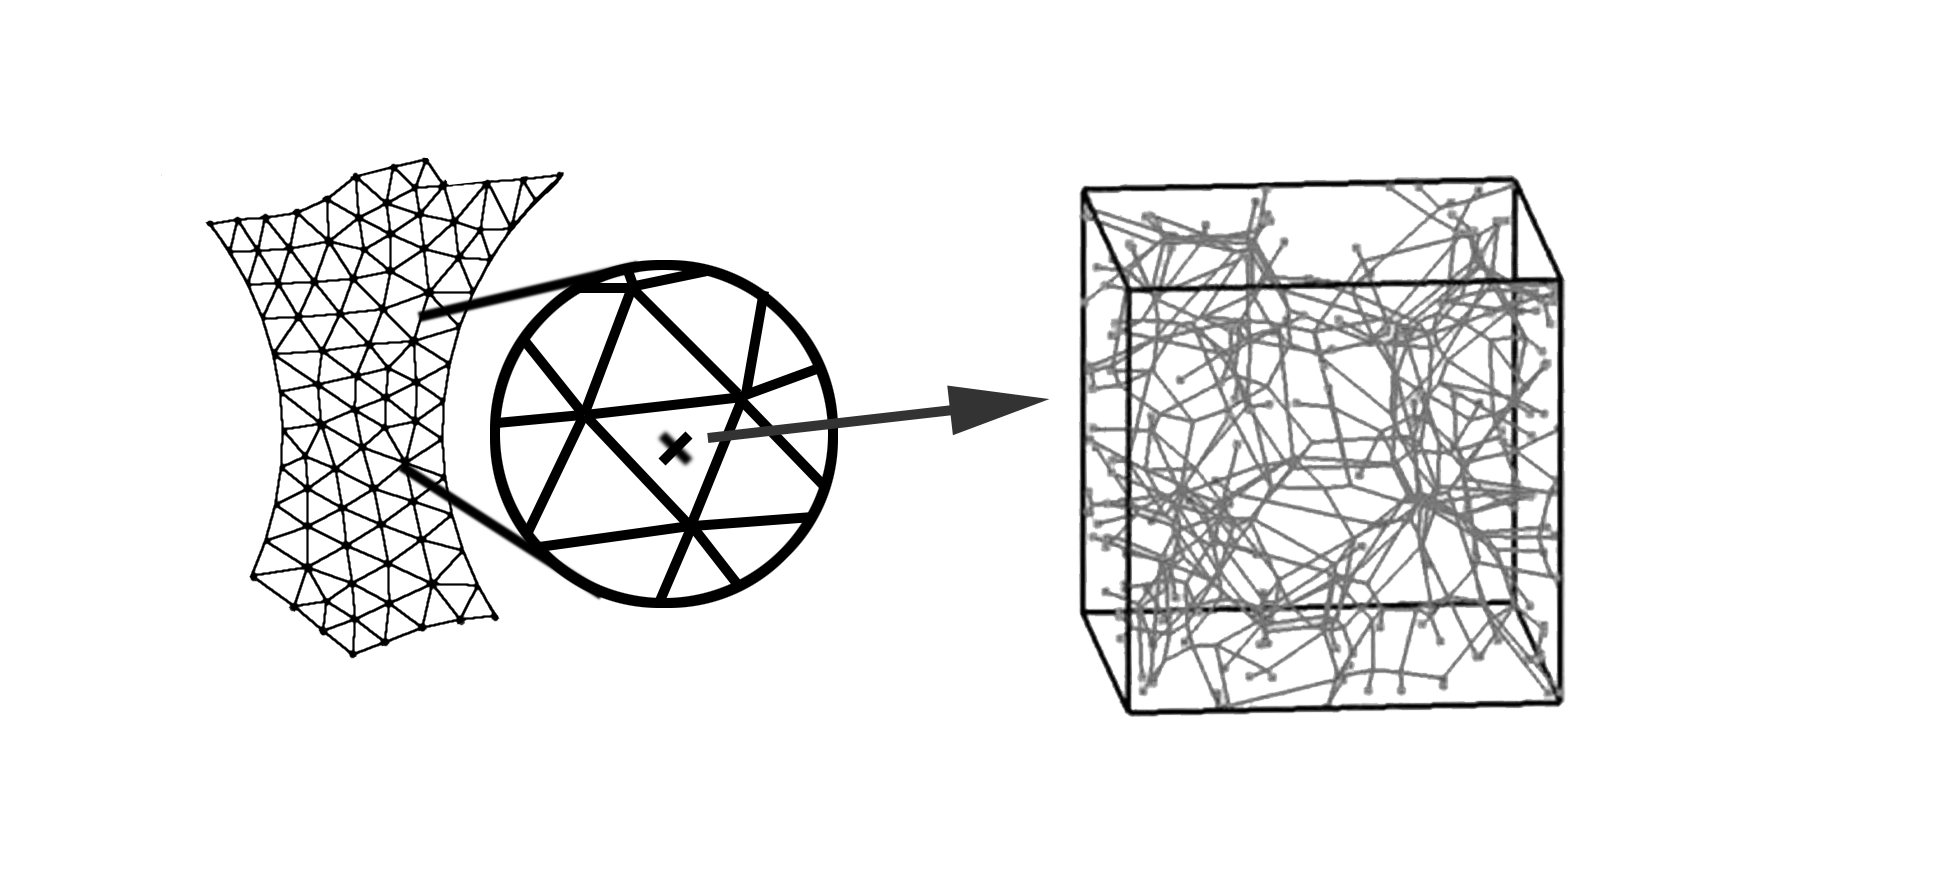
\includegraphics[height=4cm]{figure/biotissue-scales.png} 
\end{array}
$
\end{center}
\caption{\label{fig:scales} Schematic showing the hierarchy of scales in the multi-scale simulation}
\end{figure}
%

The macroscopic continuum and the microscopic fiber network simulation physical scales are assumed to be strongly separated allowing the application of well-defined domain relationships between the scales. Thus no runtime considerations are required with respect to domain data locality. Parallel data locality of the required coupling data must still be accounted for during simulation execution.

The macro-scale domain is discretized using an unstructured mesh that is partitioned across the parallel execution space of the scale. Figure \ref{fig:scales} depicts the relationship between the two scales with respect to the macro-scale unstructured mesh, an individual numerical integration point on that mesh, and the RVE-level microscale simulation corresponding to that macro-scale location.

\red{refer back to earlier parts of the paper and be specific about what AMSI controls in those parts}

At each macro-scale numerical integration point, the deformation gradient $F$ is calculated and provided to the AMSI coupling system, which uses a communication plan to provide the value to the micro-scale RVE simulation. This value is used by the micro-scale as shown in equation \ref{eq:downscaling} to establish the boundary conditions for the current state of the micro-scale RVE problem. Once a solution has been reached for the micro-scale simulation, the macro-scale stress term $\sigma^{(M)}$ from equation \ref{eq:macro_stress_discrete} and the macro-scale stress divergence term $\div \sigma^{(M)}$ from equation \ref{eq:macro_stress_divergence} are supplied to AMSI. These terms are communicated to the macro-scale and associated with the coupled integration point for use in assembling the macro-scale linear algebraic system for the current Newton iteration.

Up- and down-scaling transformations of the coupling data currently occurs in user code after (or before) employing the communication plan. The down-scaling of the deformation gradient terms to generate the displacement on the corner of an RVE in equation \ref{eq:downscaling} takes place at micro-scale after the coupling communication. The up-scaling in equation \ref{eq:macro_stress_discrete} also takes place at micro-scale, prior to communicating the stress terms to the macro-scale.

\subsection{Problem Specification}\label{sec:specification}
\red{size of the problem, description of setup and params}


%%%%%%%%%%%%%%%%%%%%%%%%%%%%%%%%%%%%%%%%%%%%%%%%%%%%%%%%%%%%%%%%%%%%%%
\section{Results}
\label{sec:results}

The embedded neuron model described above provides local strain information within the neuron structure that is inaccessible by current experimental procedures. Such strain information can be used to examine an embedded neuron structure's susceptibility to injury, which provides physiological insights about the cause of pain when an innervated ligament is excessively loaded. \red{Sijia, Beth, Victor B.: How representative is this one neuron configuration that we study? Can we extrapolate these results to other studies?} 

For this study, the collagen gel surrounding the neuron structure is subjected to bulk strains of up to 16$\%$, which corresponds to painful ligament loading \citep{Zhang:2016ga}. The strain within the neuron structure is quantified by a complementary cumulative distribution function (ccdf) defined as 
%
\begin{equation}
\text{ccdf}(X) = \int_{X}^{\infty} p_{\epsilon^*}(X)d\epsilon^* = \text{Pr}[ \epsilon^*\le X],
\label{eq:ccdf}
\end{equation}
%
where $p_{\epsilon^*}(X)$ is the probability density function of $\epsilon^*$ and $\epsilon^*$ is either the maximum principal strain (MPS) normalized by the applied bulk strain on the surrounding gel ($\epsilon_{\text{max}}/\epsilon_{\text{bulk}}$) or the MPS itself ($\epsilon_{\text{max}}$). When $\epsilon^* = \epsilon_{\text{max}}/\epsilon_{\text{bulk}}$, the applied bulk strain on the surrounding gel is amplified in the neuron structure when $\epsilon^* > 1$. When the local-strain amplification is large, moderate loads that are applied to the surrounding gel can give rise to injury in the neuron. Equation \ref{eq:ccdf} is the probability that the neuron structure (equivalent to the volume fraction of the neuron) experiences a local-strain amplification ($\epsilon^* = \epsilon_{\text{max}}/\epsilon_{\text{bulk}}$) or local-strain ($\epsilon^* = \epsilon_{\text{max}}$) of \textit{at least} $X$. 

%=========================================================================================================
\subsection{Strain Distribution}
In this section, the MPS of the embedded neuron structure is examined. For this analysis, the surrounding gel is loaded parallel to the 0 degree axis indicated in Fig.\ \ref{fig:analysis_schematic} and the axial stiffness in the cell body, $E_A^{\text{cell}}$, is set by Eq.\ \eqref{eq:cellEA} with $t=30$. 
%
\begin{figure}[ht]
\begin{center}
$
\begin{array}{c}
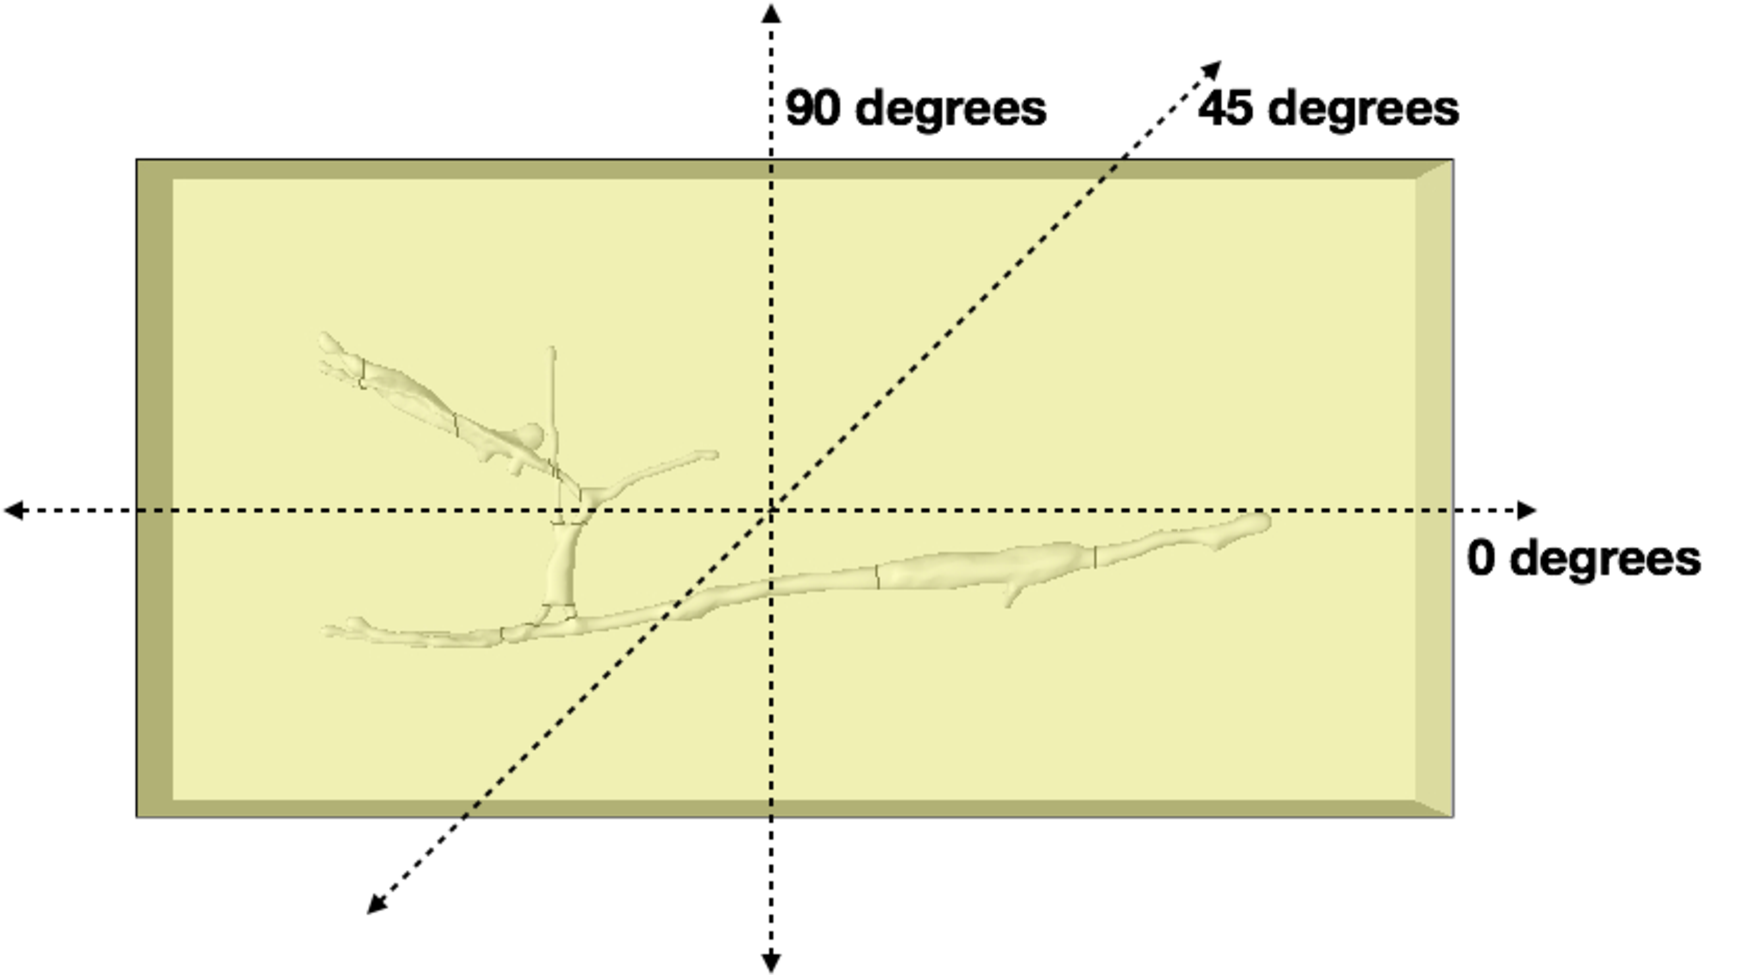
\includegraphics[height=4cm]{figure/AngleLoadingSchematic.pdf} 
\end{array}
$
\end{center}
\caption{\label{fig:analysis_schematic} Schematic showing axes of load directions corresponding to 0, 45, and 90 degrees.}
\end{figure}
%

Color maps of the MPS on the neuron structure for bulk strains of 10$\%$ (non painful ligament loading) and 16$\%$ (painful ligament loading) in the collagen gel are plotted in Fig.\ \ref{fig:neuron_0deg_MPS}.
%
% Images from N2P178/4-Neuron_FT_trcBC folder.
\begin{figure}[ht]
\begin{center}
$
\begin{array}{cc}
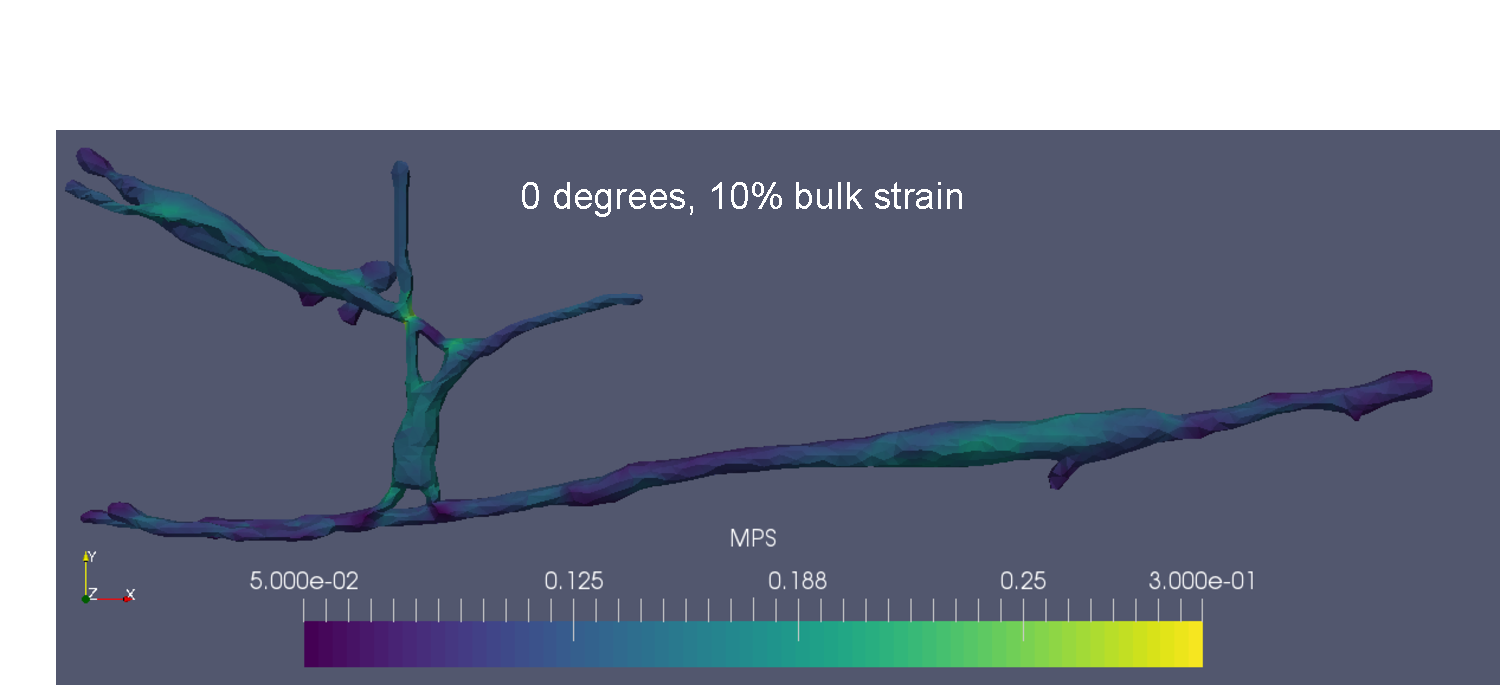
\includegraphics[height=3.25cm]{figure/MPS_rot0_strain10.pdf} & 
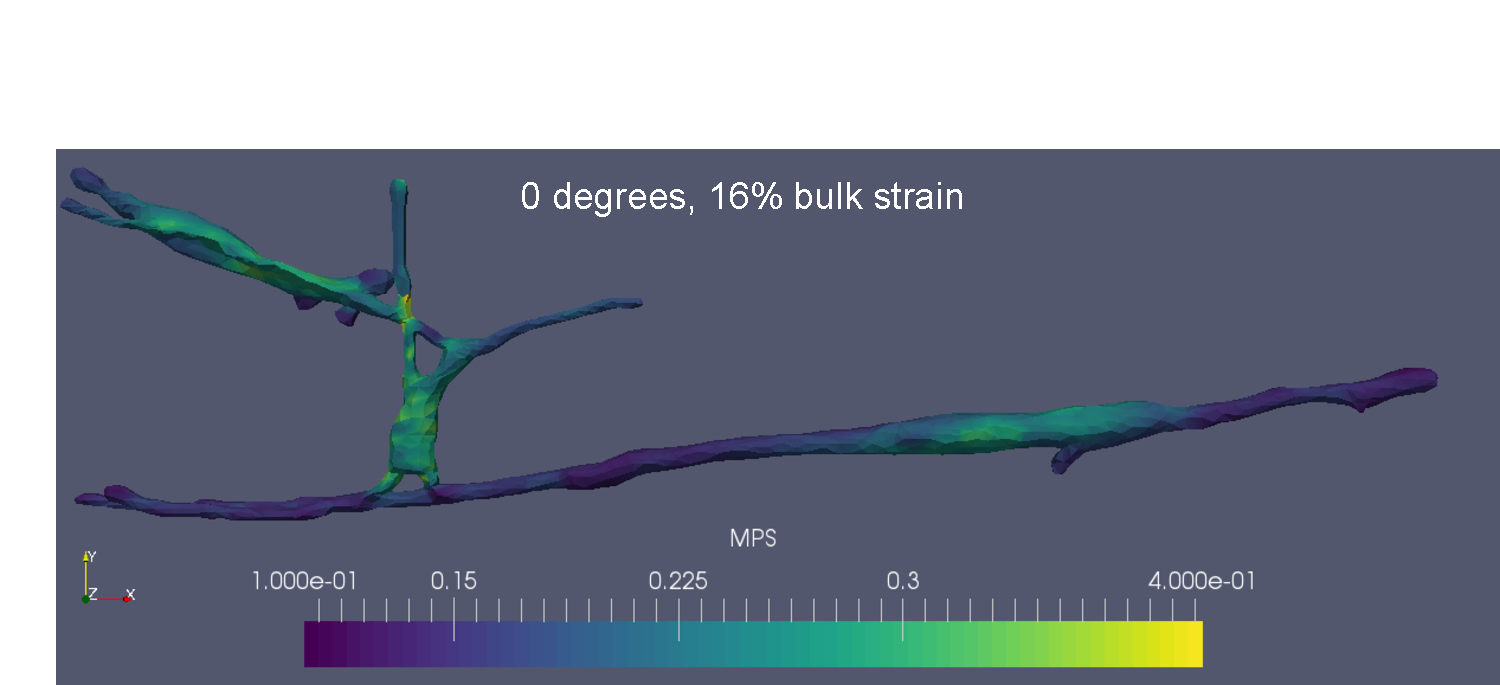
\includegraphics[height=3.25cm]{figure/MPS_rot0_strain16.pdf} \\
(a) & (b) 
\end{array}
$
\end{center}
\caption{\label{fig:neuron_0deg_MPS} Color maps of MPS plotted on neuron structure for loading angle of 0 degrees for bulk strains of (a)10$\%$ and (b) 16$\%$ in the collagen gel. The axial stiffness in the cell body is according to Eq.\ \eqref{eq:cellEA} with $t=30$. The color bar ranges from 10$\%$ to 40$\%$ MPS.}
\end{figure}
%
For both non painful and painful ligament loading, large portions of the neuron experience strains that are greater than the applied bulk strain on the surrounding gel. This indicates that the applied strains on the collagen gel are amplified in the neuron structure, which can lead to neuronal damage even when the surrounding tissue is moderately loaded. 

To gain a more quantitative understanding of the local-strain amplification in the neuron, ccdfs of the MPS in the neuron structure are plotted in Fig.\ \ref{fig:neuron_ccdf_0deg_mps} for 10$\%$ and 16$\%$ bulk strains in the collagen gel.
%
% Figure generated in N2P178/4-Neuron_FT_trcBC/MaxPrnStrn folder
\begin{figure}[ht]
\begin{center}
$
\begin{array}{c}
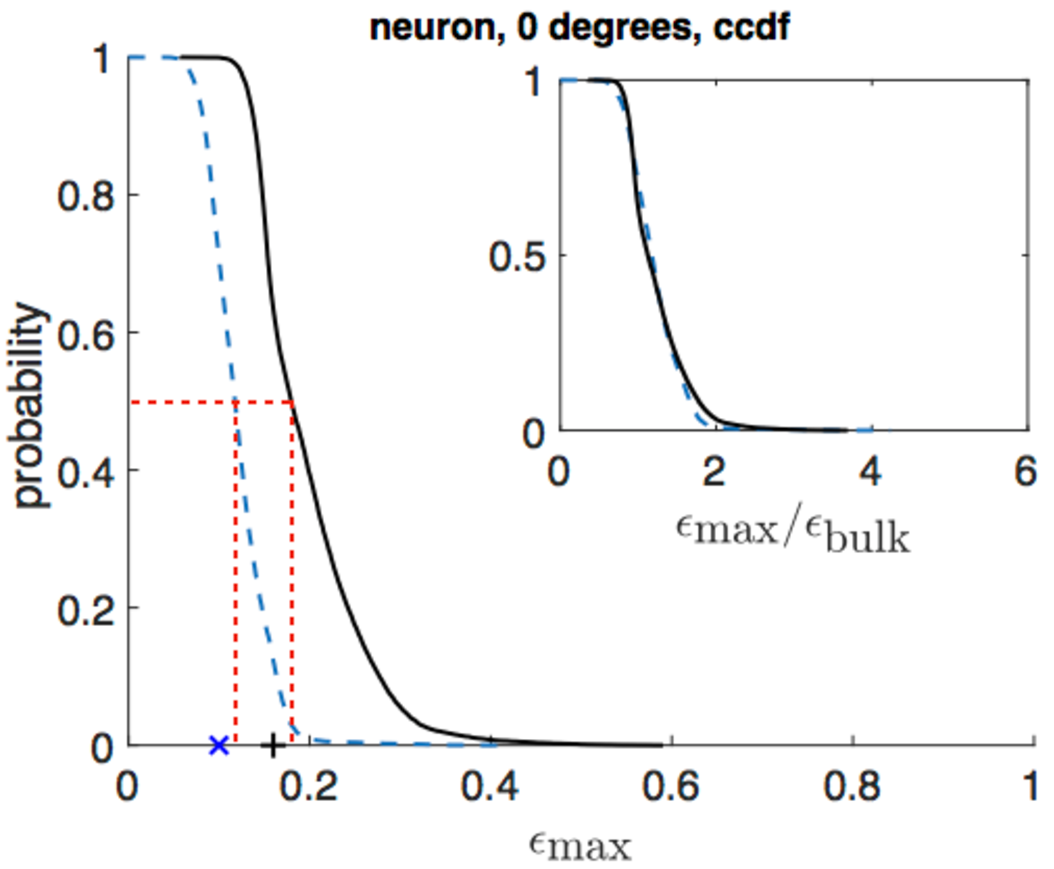
\includegraphics[height=6cm]{figure/neuron_0deg_MPS_ccdf_compare.pdf} 
\end{array}
$
\end{center}
\caption{\label{fig:neuron_ccdf_0deg_mps} Probability that MPS in the neuron structure is greater than $\epsilon_{\text{max}}$. The probability that the MPS normalized by the applied bulk strain is greater than $\epsilon_{\text{max}}/\epsilon_{\text{bulk}}$ is plotted in the inset. The distributions for bulk strains of 10$\%$ (dashed blue line) and 16$\%$ (solid black line) in the collagen gel are plotted. The averages (50$\%$ probability) are indicated by the dashed red lines. }
\end{figure}
%
For both non painful and painful ligament loading, the average MPS in the neuron structure is greater than the applied bulk strain on the collagen gel. The strain distributions shift to the right with larger bulk strain, but the normalized strain distributions (shown in the inset) are nearly the same. Volume fractions of the neuron structure corresponding to different strain amplifications are listed in Table \ref{table:ccdf_volfrac_0deg}. 
%%%%%%%%%%%%%%%%%%%%%%%%%%%%%%%%%%%%%%%%%%%%%%%%%%%%%%%%
\begin{table}[ht]
\begin{center}
\begin{tabular}{ c c c }
\hline\hline
strain amplification & vol. frac. for $\epsilon_{\text{bulk}}=0.1$ & vol. frac. for $\epsilon_{\text{bulk}}=0.16$ \\
\hline 
1 & 70$\%$ & 63$\%$ \\ 
1.5 & 18$\%$ & 21$\%$ \\
2 & 0.9$\%$ &  3.2$\%$ \\ 
3 & 0.2$\%$ & 0.2$\%$ \\ \hline \hline
\end{tabular}
\end{center}
\caption{Volume fractions of the neuron structure corresponding to different strain amplifications under non painful ($\epsilon_{\text{bulk}}=0.10$) and painful ($\epsilon_{\text{bulk}}=0.16$) ligament loading.}
\label{table:ccdf_volfrac_0deg}
\end{table}
%%%%%%%%%%%%%%%%%%%%%%%%%%%%%%%%%%%%%%%%%%%%%%%%%%%%%%%%
As seen in Table \ref{table:ccdf_volfrac_0deg}, less than 1$\%$ and 3.2$\%$ of the neuron structure experiences a local-strain amplification of more than two times for 10$\%$ and 16$\%$ applied bulk strain, respectively. The volume fraction of the neuron structure that experiences a three times local-strain application drops to 0.2$\%$ for both 10$\%$ and 16$\%$ applied bulk strain.

%=========================================================================================================
\subsection{Effect of Changing the Axial Stiffness in the Cell Body}
\label{sec:cellbody_stiffness}
The transition in the axial stiffness of the cell bodies presented in Eq.\ \eqref{eq:cellEA} is artificial. To understand how this transition affects the final strain distribution in the neuron structure, the transition rate is varied by adjusting $t$ in Eq.\ \eqref{eq:cellEA}. As seen from Eq.\ \eqref{eq:cellEA}, the value of $t$ needs to be greater than $D$ (=25.5 $\mu$m) in order for $E_A^{\text{cell}}$ to be positive. Consequently, three values of $t$ are considered: $t=$ 28 $\mu$m, 30 $\mu$m, and 50 $\mu$m, which correspond to axial stiffnesses of approximately 6.25 kPa, 10.5 kPa, and 34.3 kPa, respectively, at the center of the largest cell body in the neuron structure. The ccdfs for different axial stiffnesses of the cell body (different values of $t$) are plotted in Fig.\ \ref{fig:neuron_ccdf_vary_a} for the 0 degree loading case at an applied bulk strain of 16$\%$ in the collagen gel. 
%
% Figures generated in N2P178/6-Neuron_CellStiffness/MaxPrnStrn folder
\begin{figure}[ht]
\begin{center}
$
\begin{array}{c}
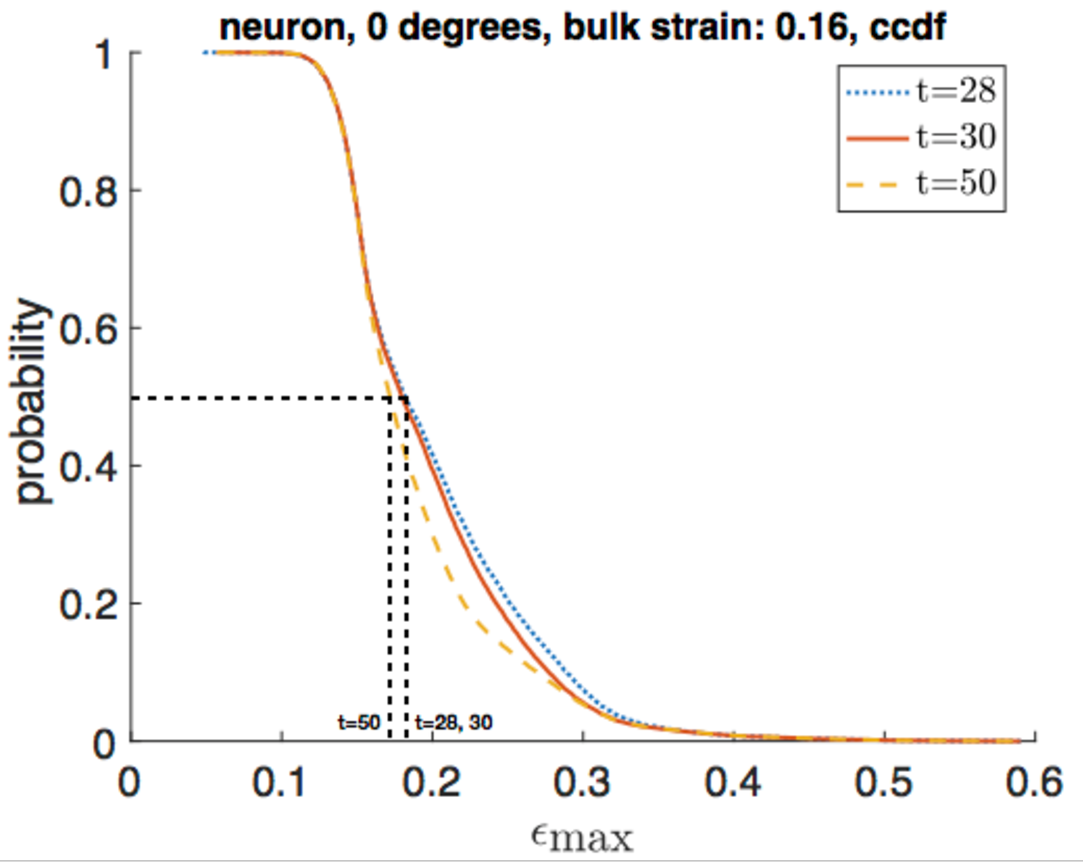
\includegraphics[height=6cm]{figure/neuron_compare_t_ccdf.pdf} 
\end{array}
$
\end{center}
\caption{\label{fig:neuron_ccdf_vary_a} Probability that MPS in the neuron structure is greater than $\epsilon_{\text{max}}$ for axial stiffnesses of cell body corresponding to t=28 (blue dotted line), 30 (red solid line), and 50 (dashed yellow line). The averages are indicated with black dashed-dotted lines. }
\end{figure}
%

As seen in Fig.\ \ref{fig:neuron_ccdf_vary_a}, the volume fraction of the neuron structure that experiences a MPS of less than he applied bulk strain (16$\%$) remains constant for all values of $E_A^{\text{cell}}$ considered. On the other hand, the volume fraction of the neuron structure that experiences a MPS of greater than the applied bulk strain decreases only slightly as $E_A^{\text{cell}}$ increases. On average, the MPS for all values of $E_A^{\text{cell}}$ considered is greater than the applied bulk strain, with approximately $1\%$ of the neuron structure experiencing local-strain amplification of more than twice the applied bulk strain. The small effect that changing $E_A^{\text{cell}}$ has on the overall strain distribution of the neuron suggests that the local-strain amplification experienced in the embedded neuron structure is not due to variations in its material properties. Therefore, the effect of neuron-structure configuration  relative to loading direction on the strain distribution is explored in the next section.

%=========================================================================================================
\subsection{Effect of Changing the Loading Direction}
\label{sec:loading_direction}
In this section, we examine how the strain distribution of the neuron structure changes when the loading direction on the collagen gel is varied. The structural features in the neuron are exposed to different modes of deformation when the loading direction is adjusted. Through this analysis, we develop insights about how the geometric configuration of the neuron structure can give rise to local-strain amplification.

The three different loading cases considered in this section are shown schematically in Fig.\ \ref{fig:analysis_schematic}(a). The effect of changing the loading angle is explored for $E_A^{\text{cell}}$ corresponding to $t$=30 in Eq.\ \eqref{eq:cellEA}. Color maps of the MPS on the neuron structure for loading angles of 45 and 90 degrees are plotted in Fig.\ \ref{fig:neuron_MPS} for bulk strains of 10$\%$ and 16$\%$ in the collagen gel.
%
% Images from N2P178/4-Neuron_FT_trcBC folder.
\begin{figure}[ht]
\begin{center}
$
\begin{array}{cc}
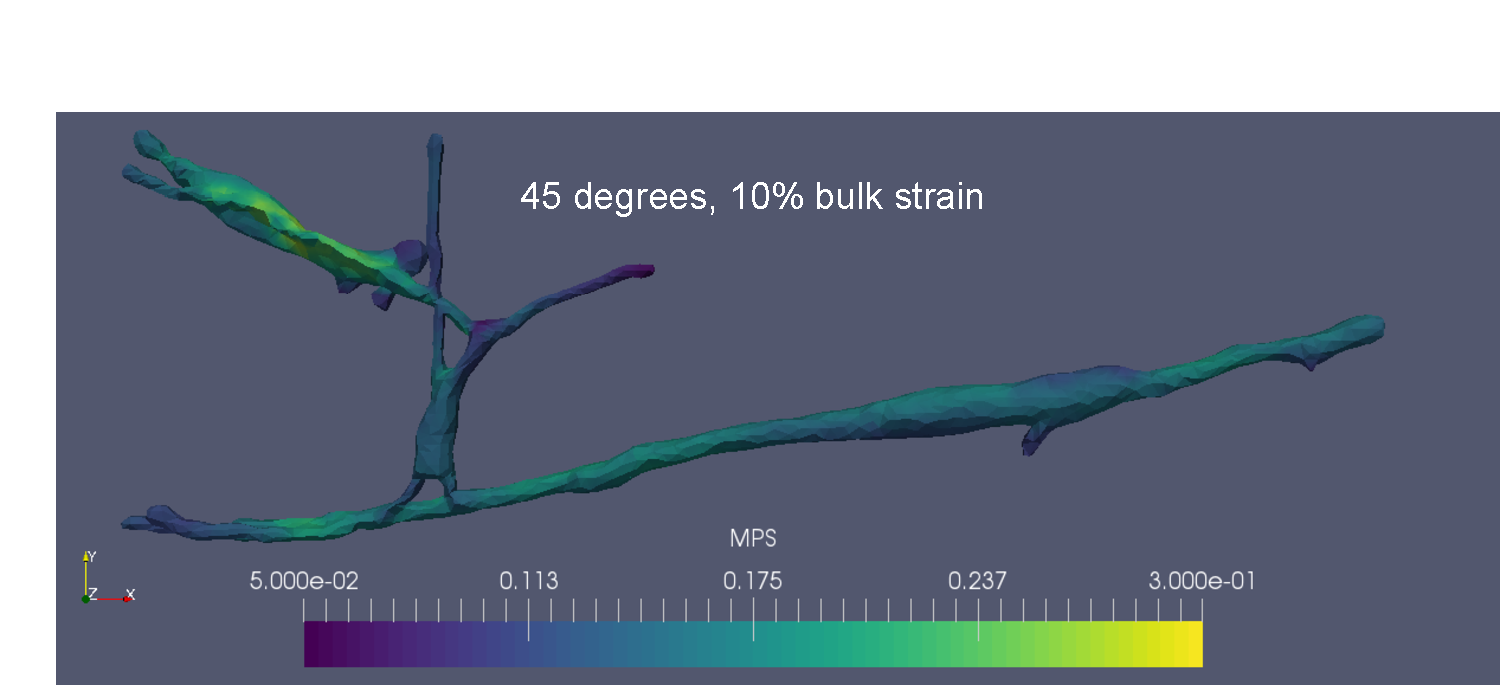
\includegraphics[height=3.5cm]{figure/MPS_rot45_strain10.pdf} &
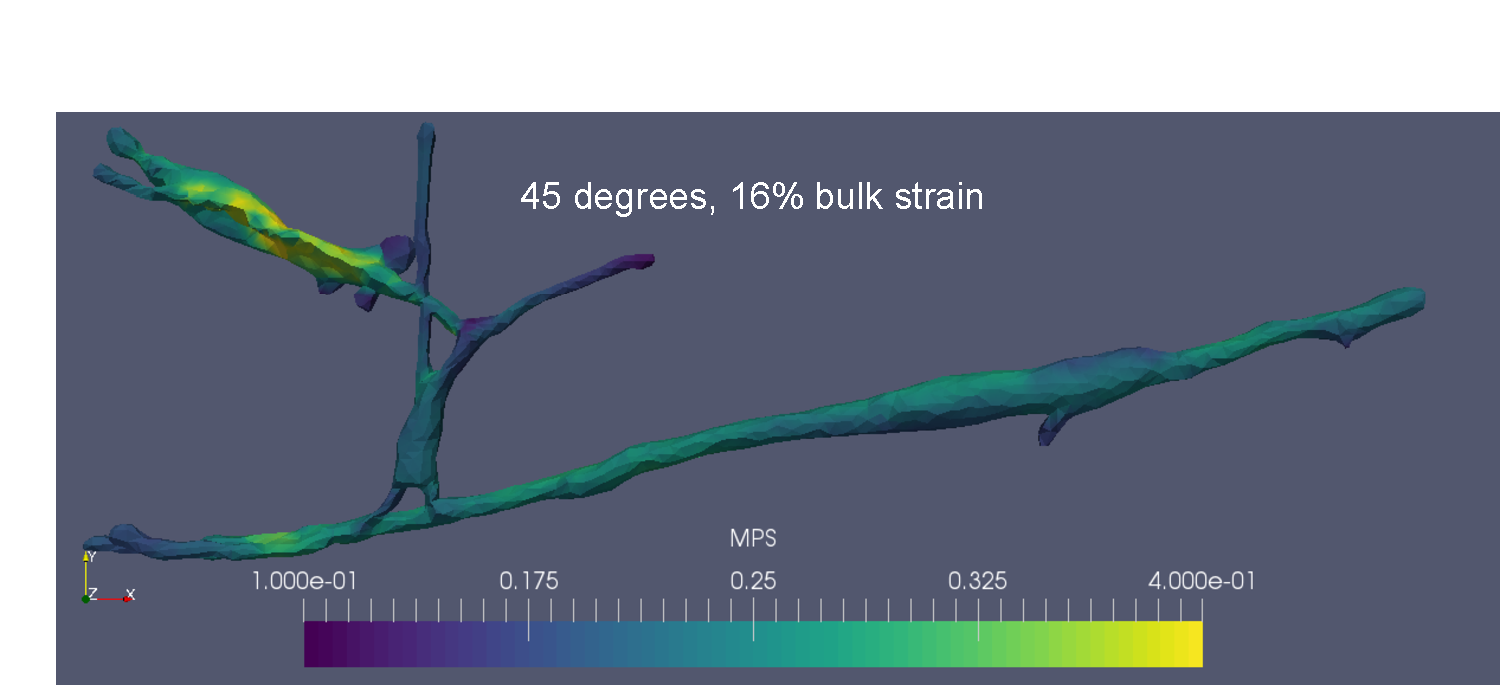
\includegraphics[height=3.5cm]{figure/MPS_rot45_strain16.pdf} \\
(a) & (b) \\
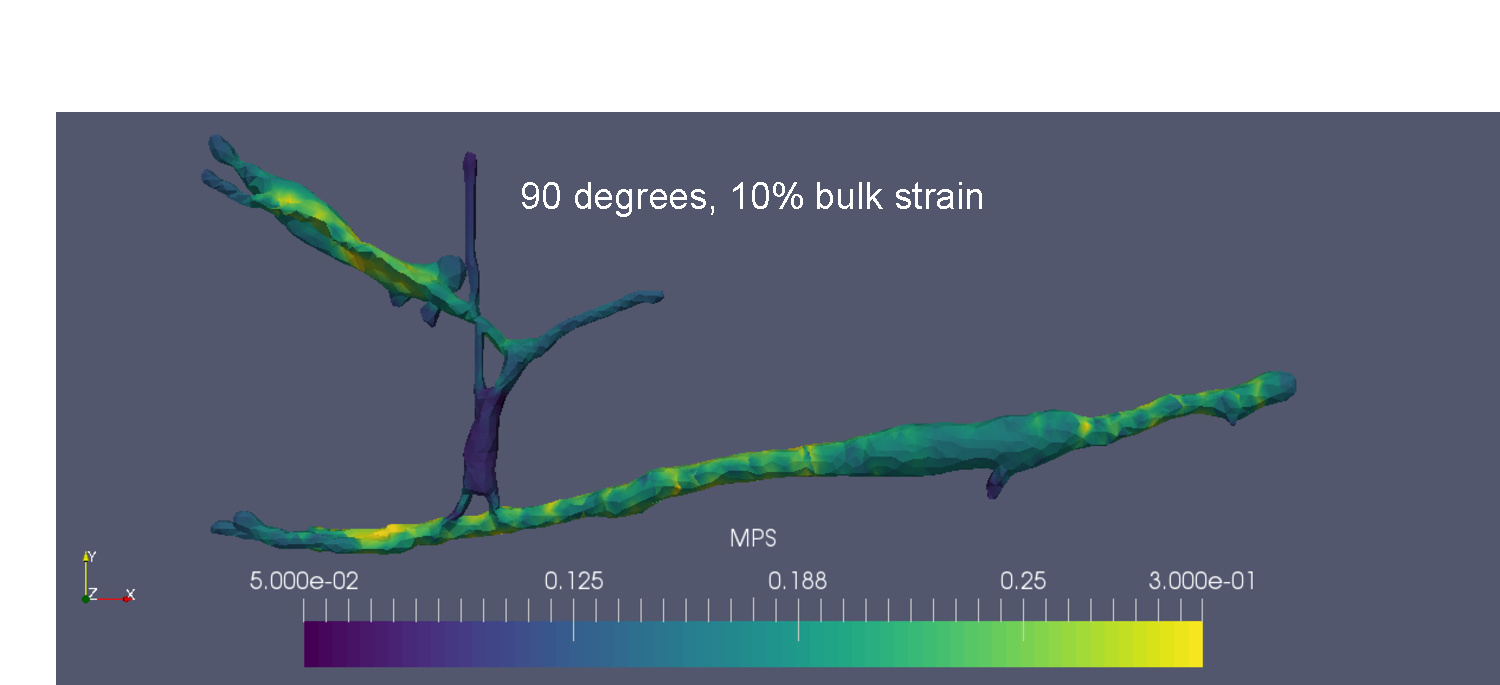
\includegraphics[height=3.5cm]{figure/MPS_rot90_strain10.pdf} & 
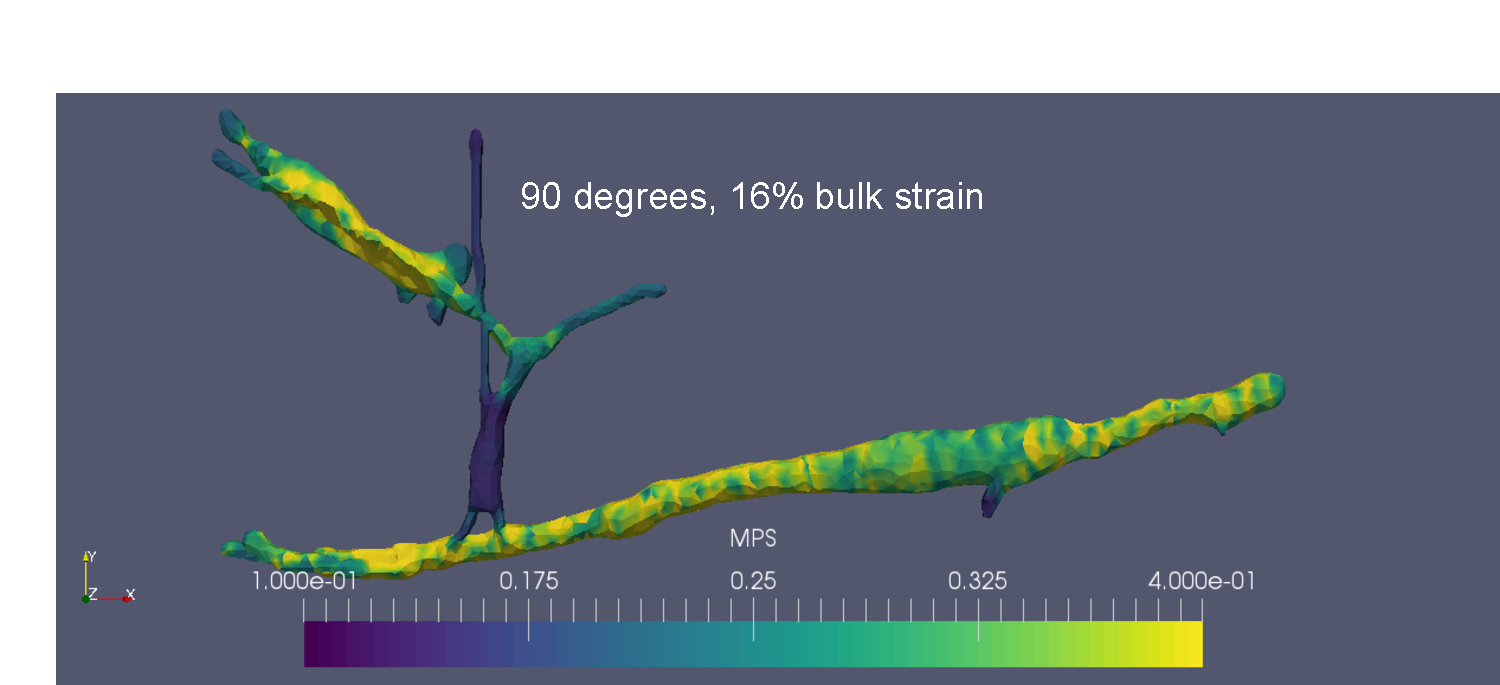
\includegraphics[height=3.5cm]{figure/MPS_rot90_strain16.pdf} \\
(c) & (d)
\end{array}
$
\end{center}
\caption{\label{fig:neuron_MPS} Color maps of maximum principal strain plotted on neuron structure for loading angles of 45 degrees (top row) and 90 degrees (bottom row) at bulk strains of 10$\%$ and 16$\%$. Color bar ranges from 10$\%$ to 40$\%$.}
\end{figure}
%

As seen in Fig.\ \ref{fig:neuron_MPS} and comparing to the 0 degree loading case in Fig.\ \ref{fig:neuron_0deg_MPS}, the strain distribution in the neuron structure varies significantly for different loading angles. In all scenarios, large portions of the neuron experience strains that are greater than the applied bulk strain in the collagen gel. The variation in strain distribution above can be quantitatively captured in ccdfs of the MPS in the neuron structure, which are plotted in Fig.\ \ref{fig:neuron_ccdf_mps} for loading angles of 45 and 90 degrees at bulk strains of 10$\%$ and 16$\%$.
%
%45 degree distributions from N2P178/4-Neuron_FT_trcBC/MaxPrnStrn/PrincipalStrainDistr.m
%90 degree distribution from N2P178/3-Neuron_FT/MaxPrnStrn/PrincipalStrainDistr_FarField.m
\begin{figure}[ht]
\begin{center}
$
\begin{array}{cc}
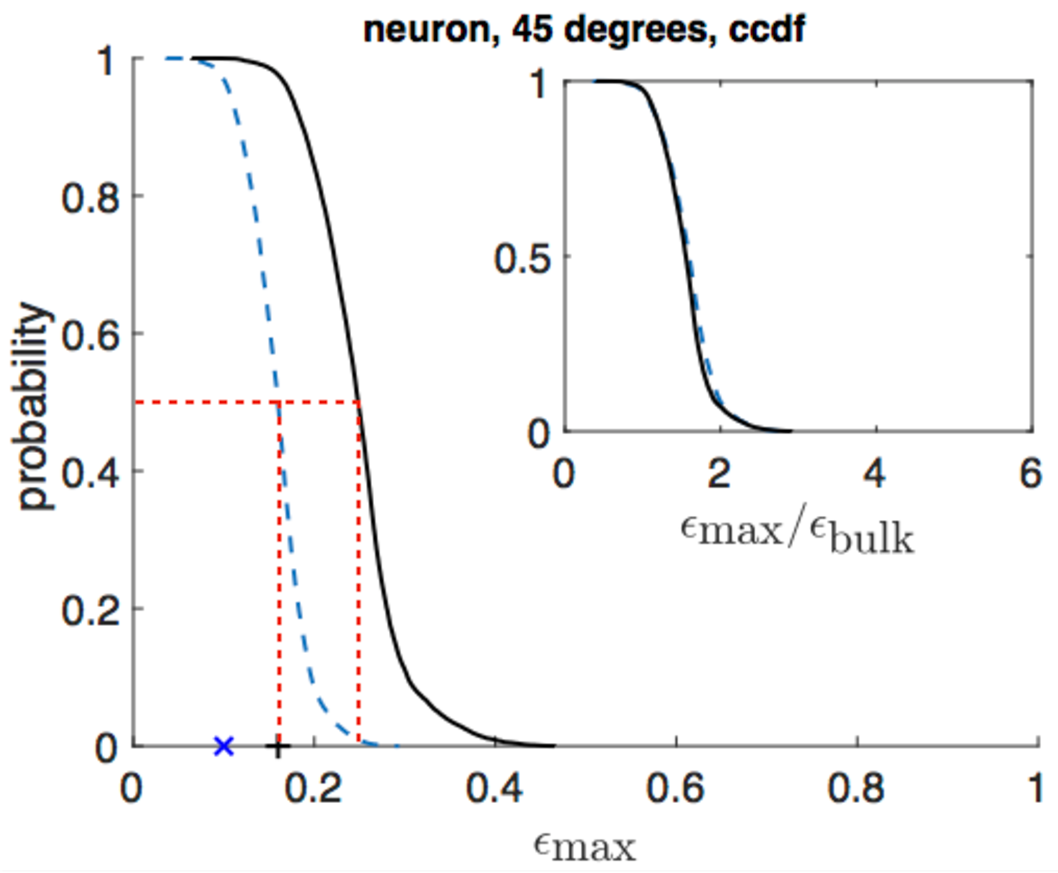
\includegraphics[height=6cm]{figure/neuron_45deg_MPS_ccdf_compare.pdf} &
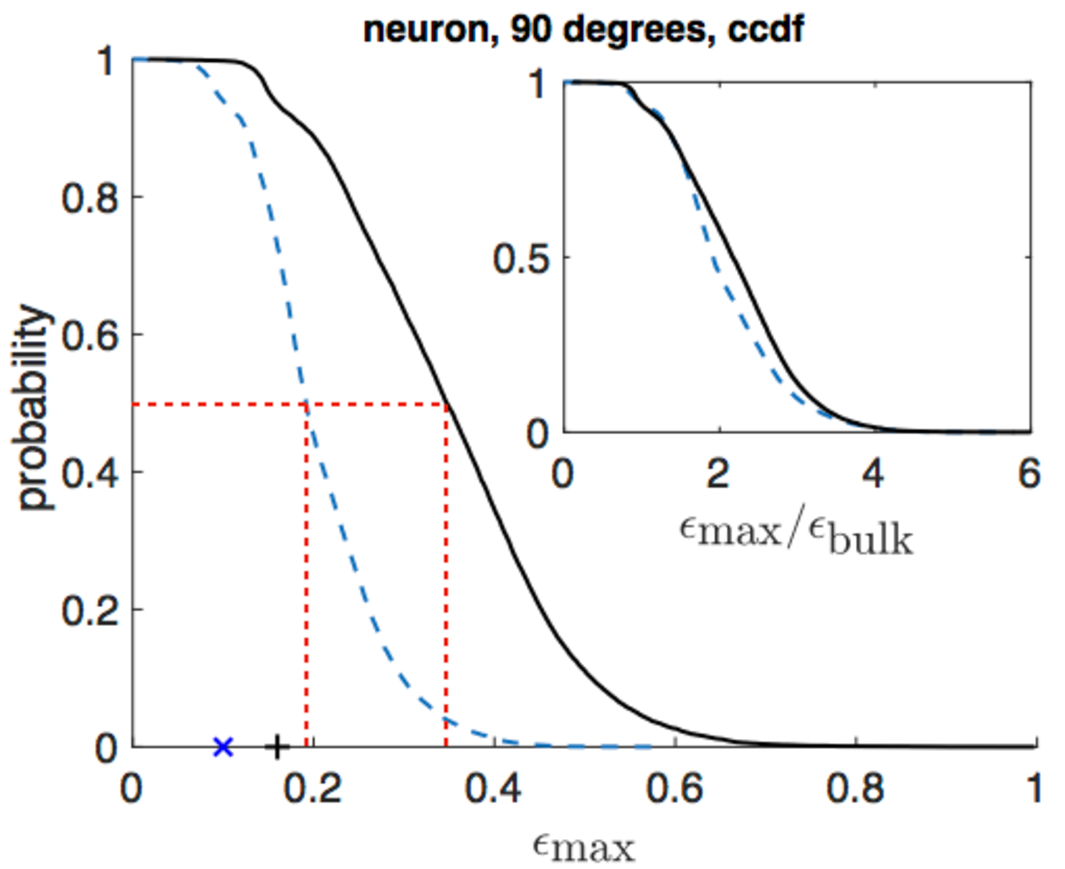
\includegraphics[height=6cm]{figure/neuron_90deg_MPS_ccdf_compare.pdf} \\
(a) & (b) 
\end{array}
$
\end{center}
\caption{\label{fig:neuron_ccdf_mps} Probability that MPS in the neuron structure is greater than $\epsilon_{\text{max}}$. The probability that the MPS normalized by the applied bulk strain is greater than $\epsilon_{\text{max}}/\epsilon_{\text{bulk}}$ is plotted in the insets. The distributions for bulk strains of 10$\%$ (dashed blue line) and 16$\%$ (solid black line) in the collagen gel are plotted for loading angles of (a) 45 and (b) 90 degrees. The averages (50$\%$ probability) are indicated by the dashed red lines. MPS corresponding to 10$\%$ and 16$\%$ are marked by blue ``x'' and black cross, respectively, on the abscissa. } 
\end{figure}
%
Consistent with what is observed in the strain distribution when comparing the color maps of Figs.\ \ref{fig:neuron_0deg_MPS} and \ref{fig:neuron_MPS}, the ccdfs vary significantly for different loading directions. 

For both non painful and painful ligament loading at 45 and 90 degrees, the average MPS in the neuron structure is greater than the applied bulk strain on the surrounding gel. The strain distributions shift to the right with larger applied bulk strain, but the normalized distributions (shown in insets) are nearly the same. Compared to the 0 degree loading case (see Fig.\ \ref{fig:neuron_ccdf_0deg_mps}), the average MPS for 45 and 90 degree loading is greater. Volume fractions of the neuron structure corresponding to different strain amplifications are listed in Table \ref{table:ccdf_volfrac_compare} for the 45 and 90 degree loading cases.
%%%%%%%%%%%%%%%%%%%%%%%%%%%%%%%%%%%%%%%%%%%%%%%%%%%%%%%%
\begin{table}[ht]
\begin{center}
\begin{tabular}{ c c c c c }
\hline\hline
& \multicolumn{2}{c}{vol. frac. for 45 degree loading} & \multicolumn{2}{c}{vol. frac. for 90 degree loading} \\ \hline 
strain amplification & $\epsilon_{\text{bulk}}=0.1$ & $\epsilon_{\text{bulk}}=0.16$ & $\epsilon_{\text{bulk}}=0.1$ & $\epsilon_{\text{bulk}}=0.16$ \\
\hline 
1 & 97$\%$ & 98$\%$ & 94$\%$ & 93$\%$\\ 
1.5 & 61$\%$ & 57$\%$ & 79$\%$ & 78$\%$\\
2 & 8.4$\%$ &  7.0$\%$ & 45$\%$ &  58$\%$\\ 
3 & 0$\%$ & 0$\%$ & 9.7$\%$ & 14$\%$\\ \hline \hline
\end{tabular}
\end{center}
\caption{Volume fractions of the neuron structure corresponding to different strain amplifications under non painful ($\epsilon_{\text{bulk}}=0.10$) and painful ($\epsilon_{\text{bulk}}=0.16$) ligament loading at 45 and 90 degrees.}
\label{table:ccdf_volfrac_compare}
\end{table}
%%%%%%%%%%%%%%%%%%%%%%%%%%%%%%%%%%%%%%%%%%%%%%%%%%%%%%%%
From Table \ref{table:ccdf_volfrac_compare}, the volume fraction of the neuron structure that experiences a local-strain amplification of more than two times when loaded at 45 and 90 degrees is significantly larger than in the 0 degree loading case.

Although the average strain amplification in the neuron structure is greater when loaded at 45 degrees than when loaded at 0 degrees, the tail of the strain distribution for the 45 degree case is shorter with a maximum strain amplification that is less than three times. In the 90 degree loading case, the average strain amplification is nearly double for non painful loading and more than double for painful loading. The tail of the distribution is significantly longer for the 90 degree loading case with 9.7$\%$ and 15$\%$ of the neuron structure experiencing strain amplifications of three times for non painful and painful ligament loading, respectively.

%Variation in the shape and spread of the neuron strain distributions at different bulk strains is greatest in the case of 90 degree loading, where the spread of the distributions increase with larger bulk strain. In contrast, the variations in shape and spread of the neuron strain distributions are small for the 0 and 45 degree loading cases. Additional insight can be gained by separating the neuron strain distribution into contributions from the cell bodies and axons. The distributions of maximum principal strain in the cell bodies and axons are plotted in Fig.\ \ref{fig:rgns_ccdf_mps}.
%%
%\begin{figure}[ht]
%\begin{center}
%$
%\begin{array}{ccc}
%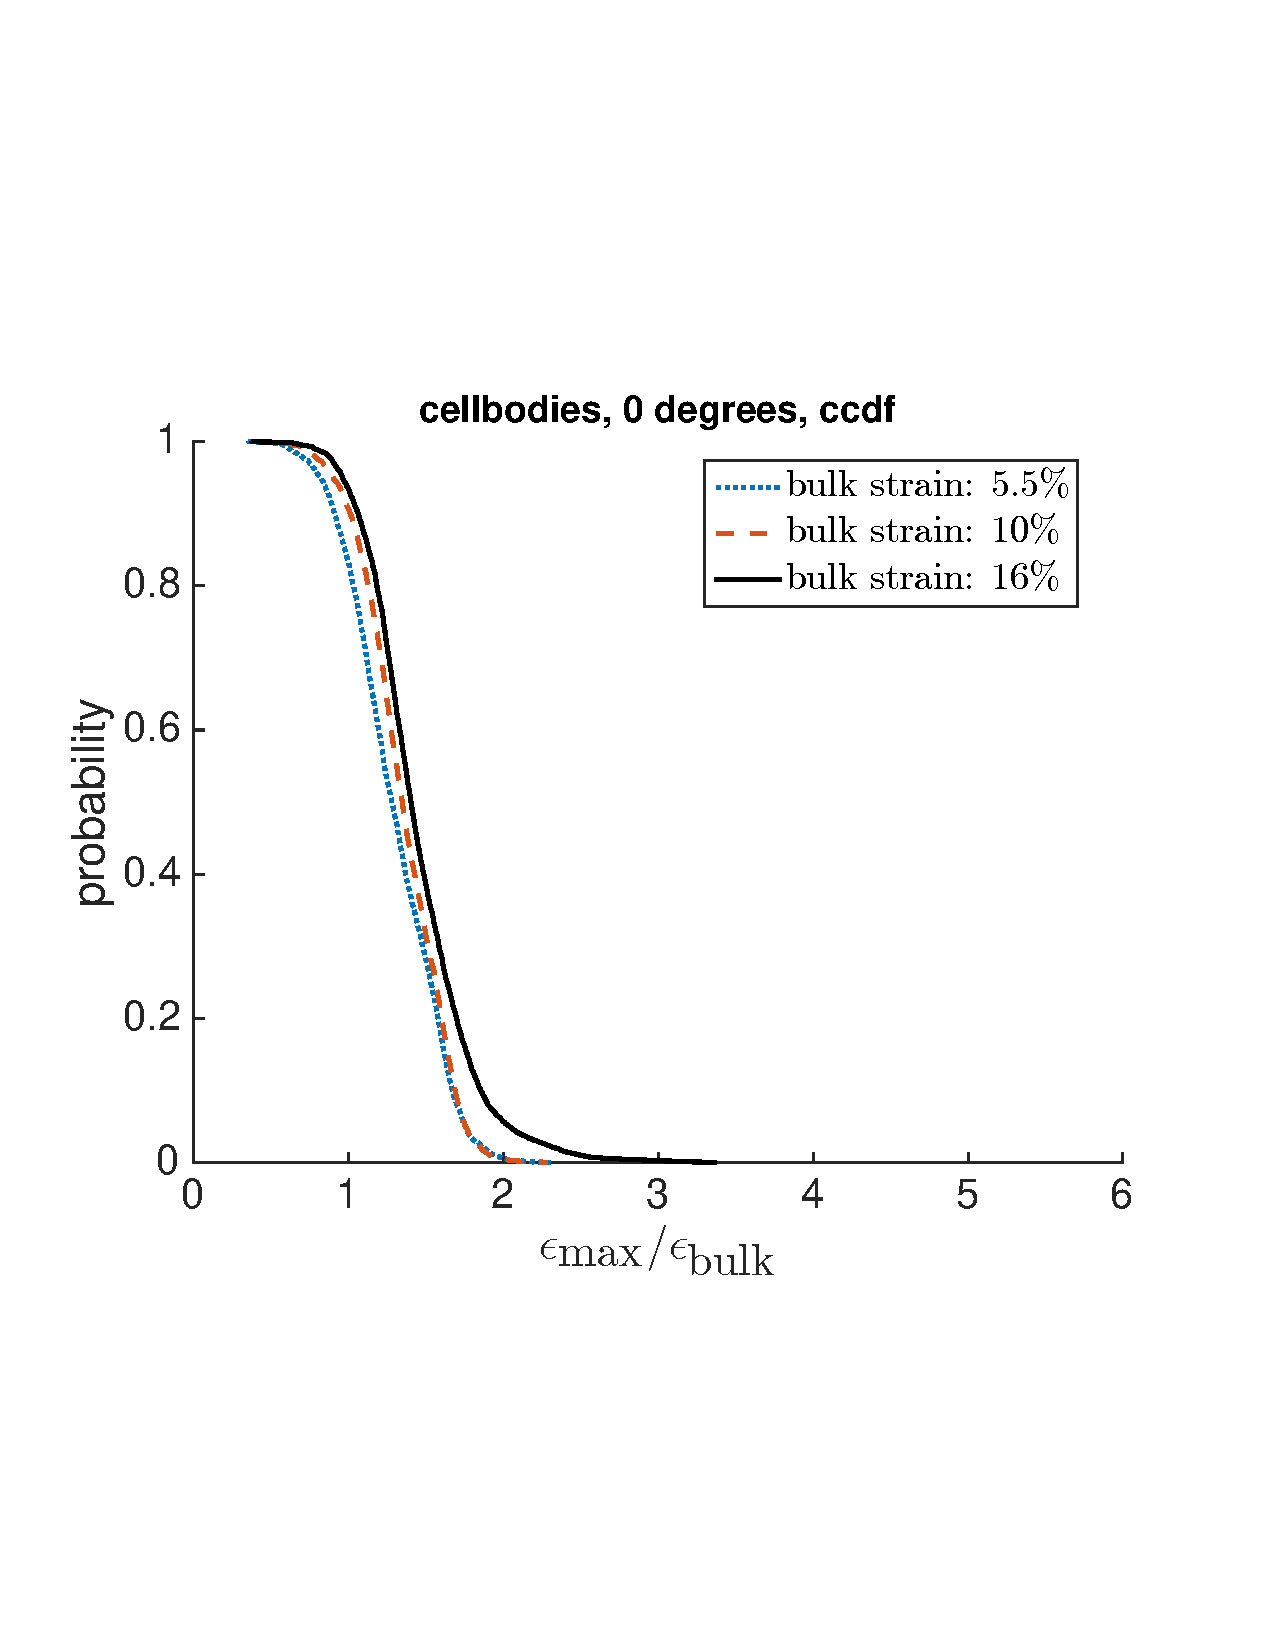
\includegraphics[height=4.5cm]{figure/rot0_FT50_128_1920_ccdf_cellbodies_compare_stps.pdf} & 
%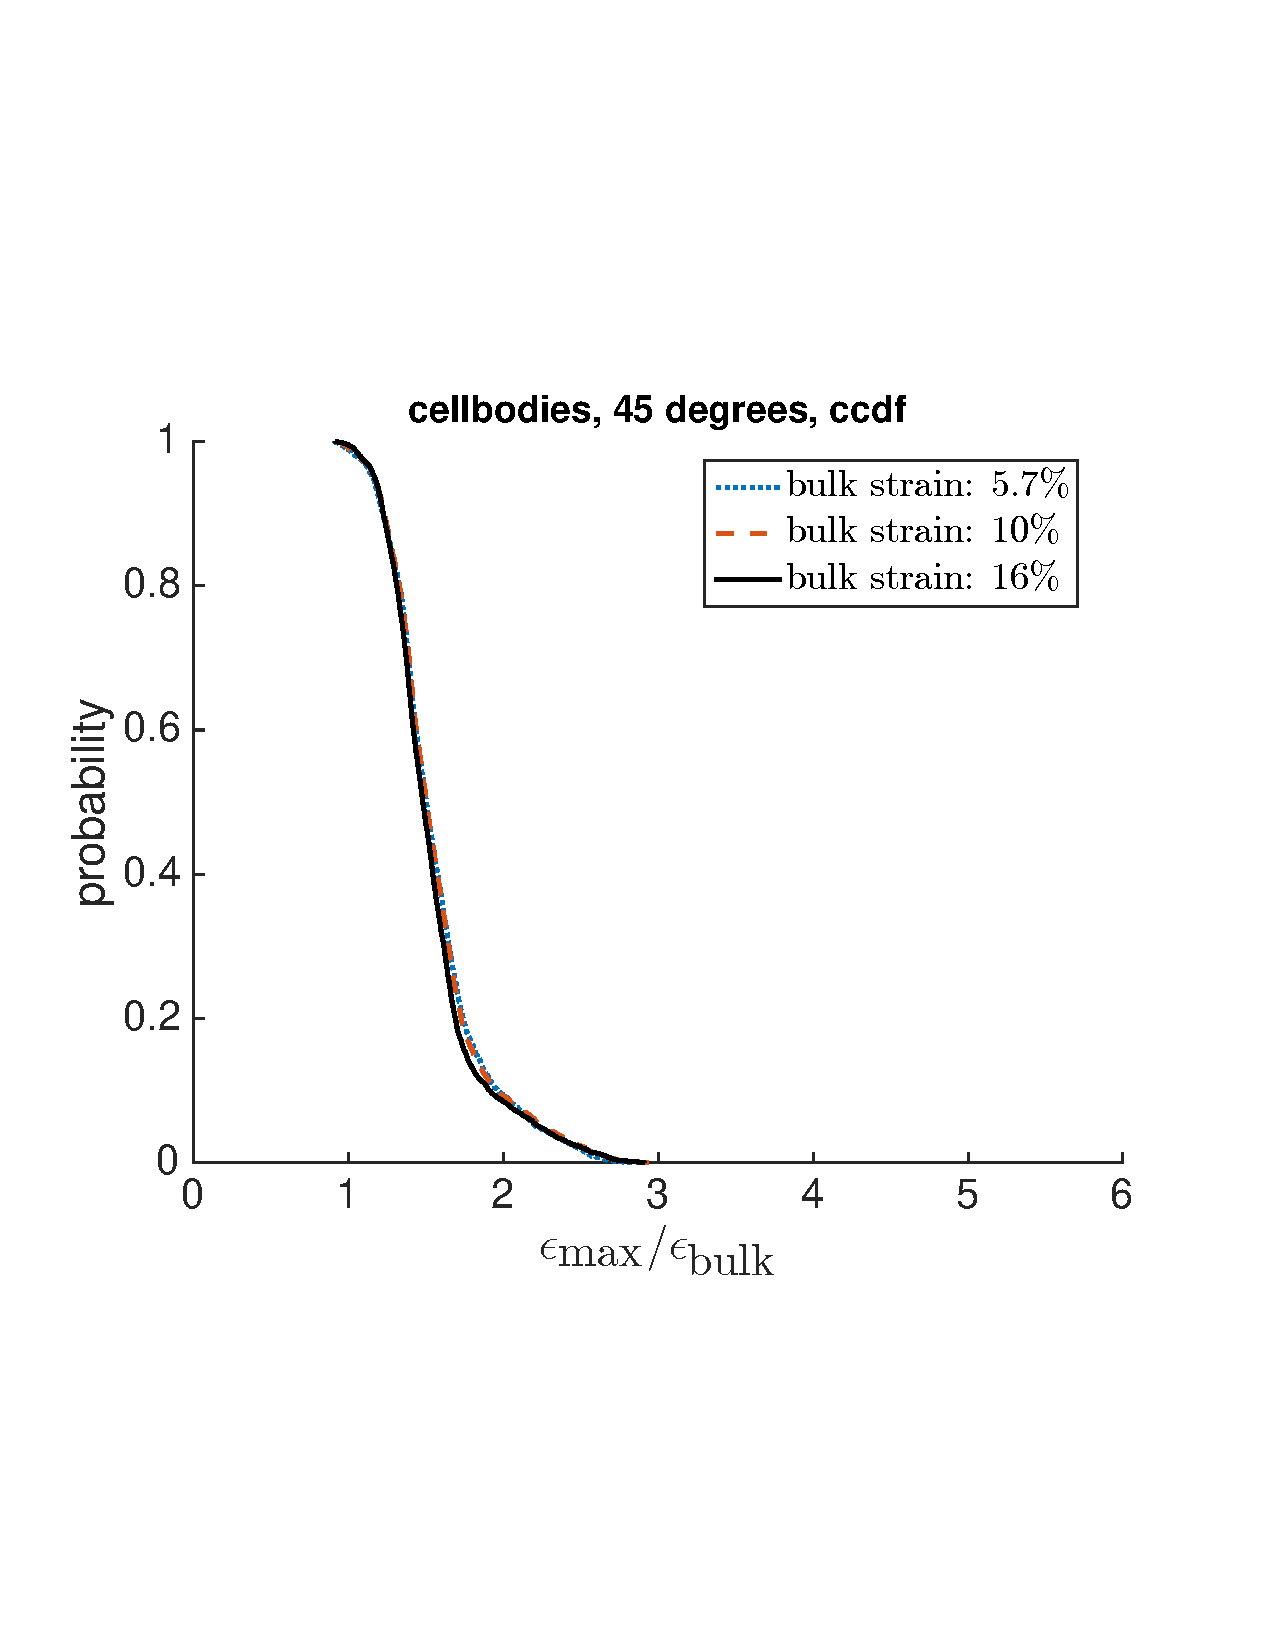
\includegraphics[height=4.5cm]{figure/rot45_FT50_128_1920_ccdf_cellbodies_compare_stps.pdf} & 
%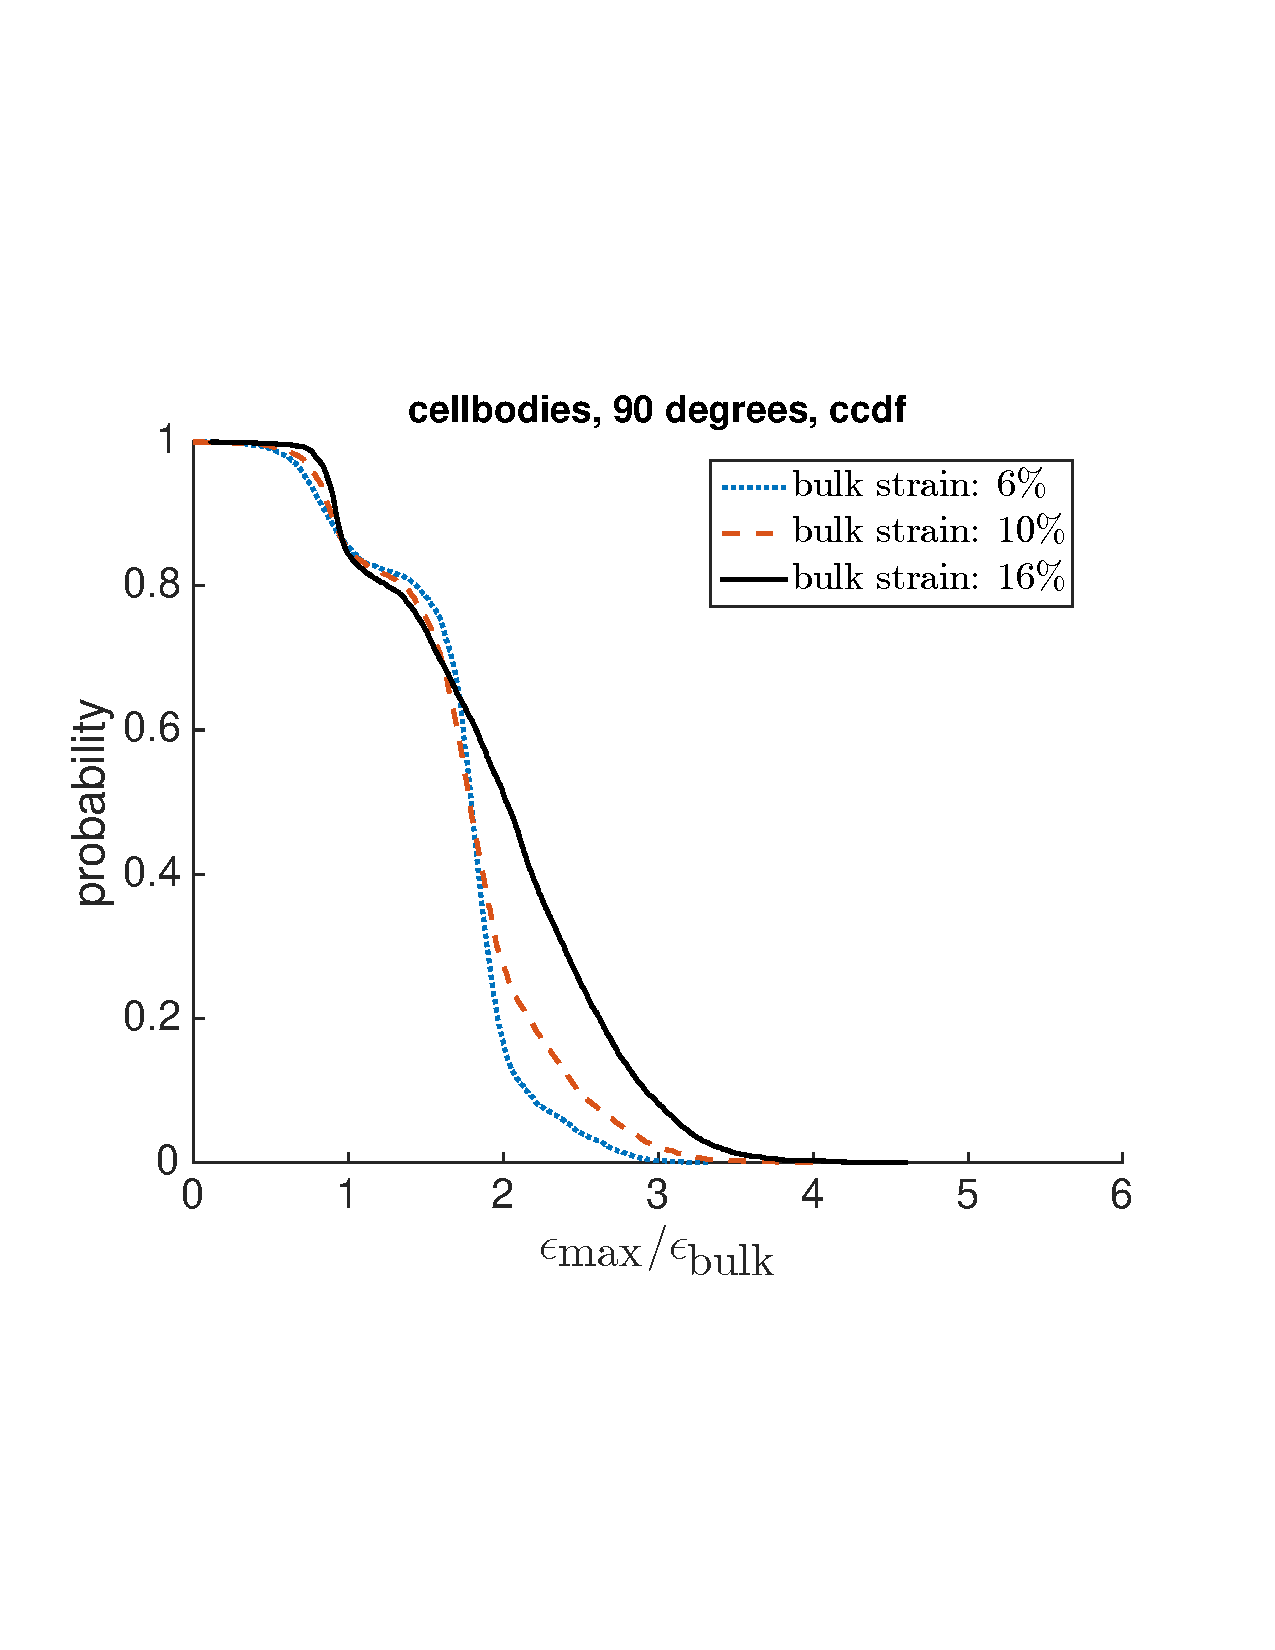
\includegraphics[height=4.5cm]{figure/rot90_FT_dspBC50_a30_128_1920_ccdf_cellbodies_compare_stps_farfield.pdf} \\
%(a) & (b) & (c) \\
%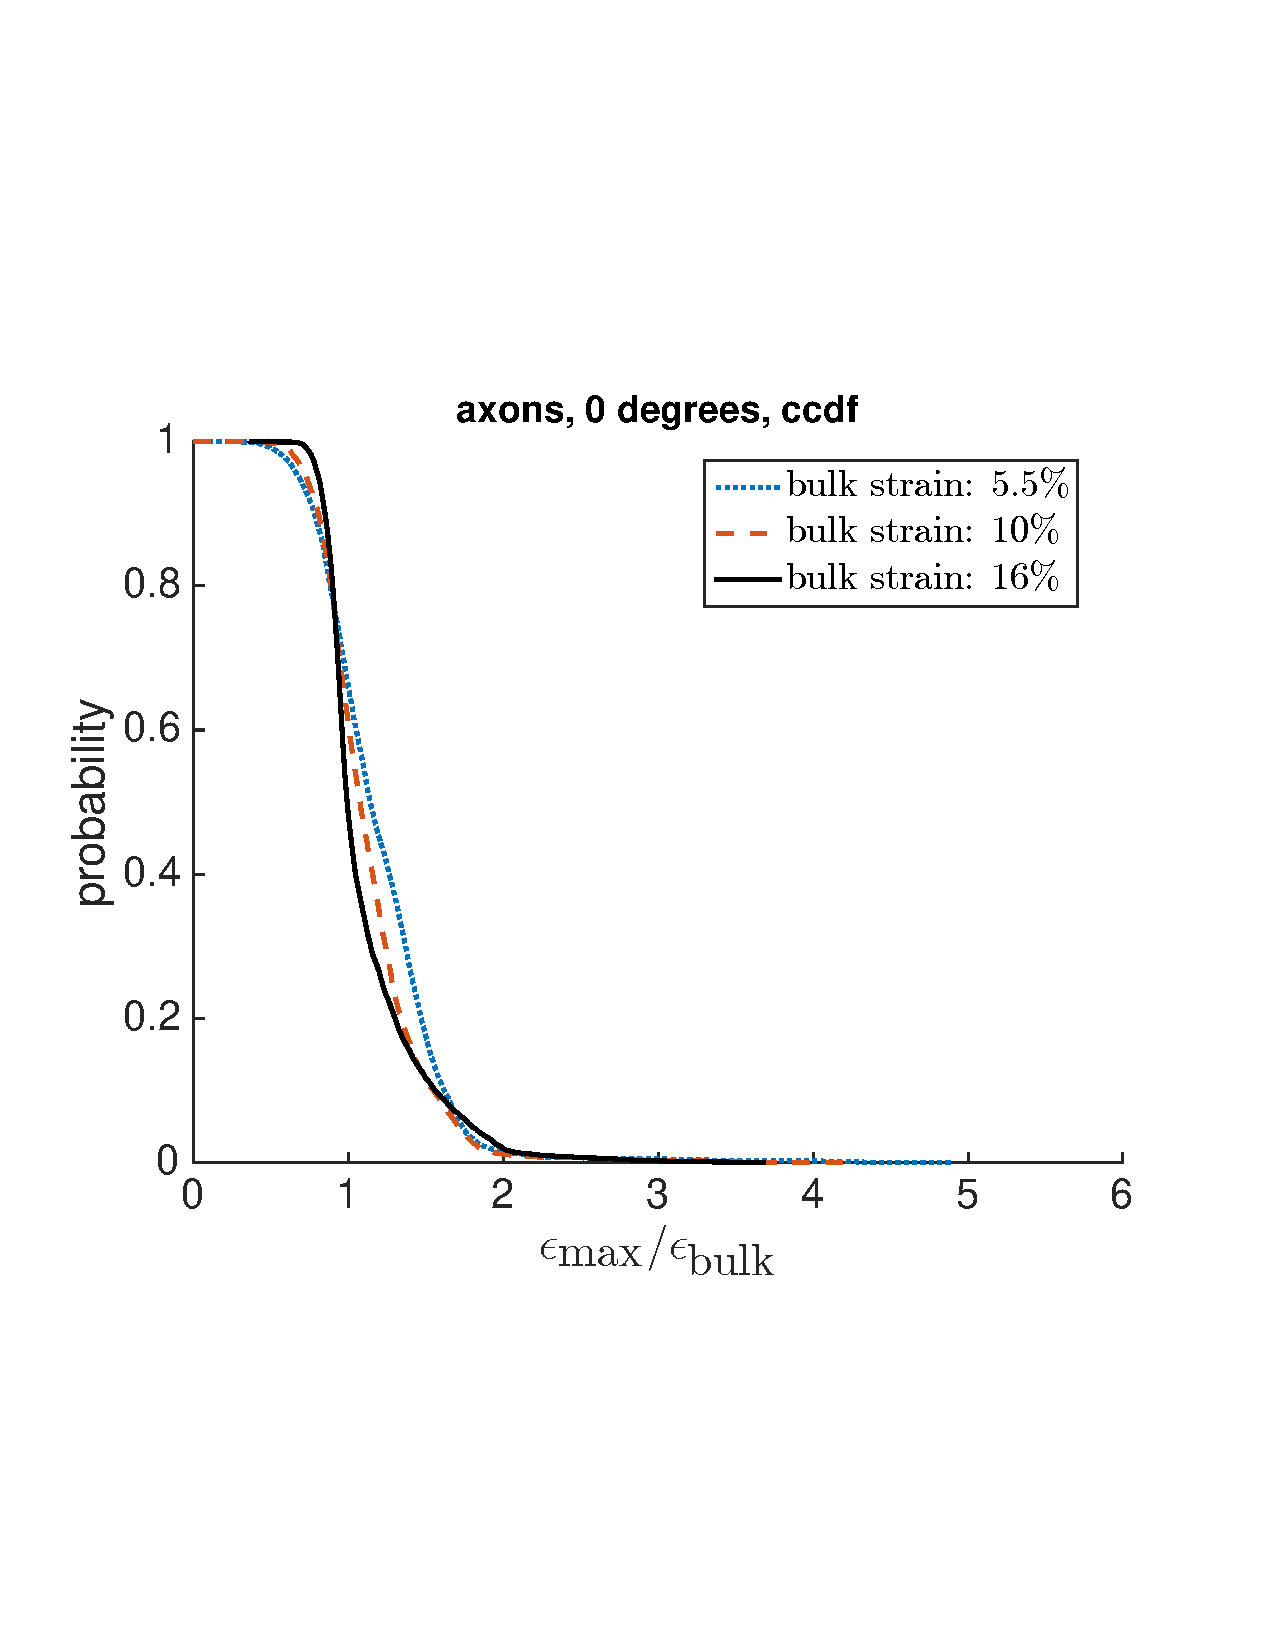
\includegraphics[height=4.5cm]{figure/rot0_FT50_128_1920_ccdf_axons_compare_stps.pdf} &
%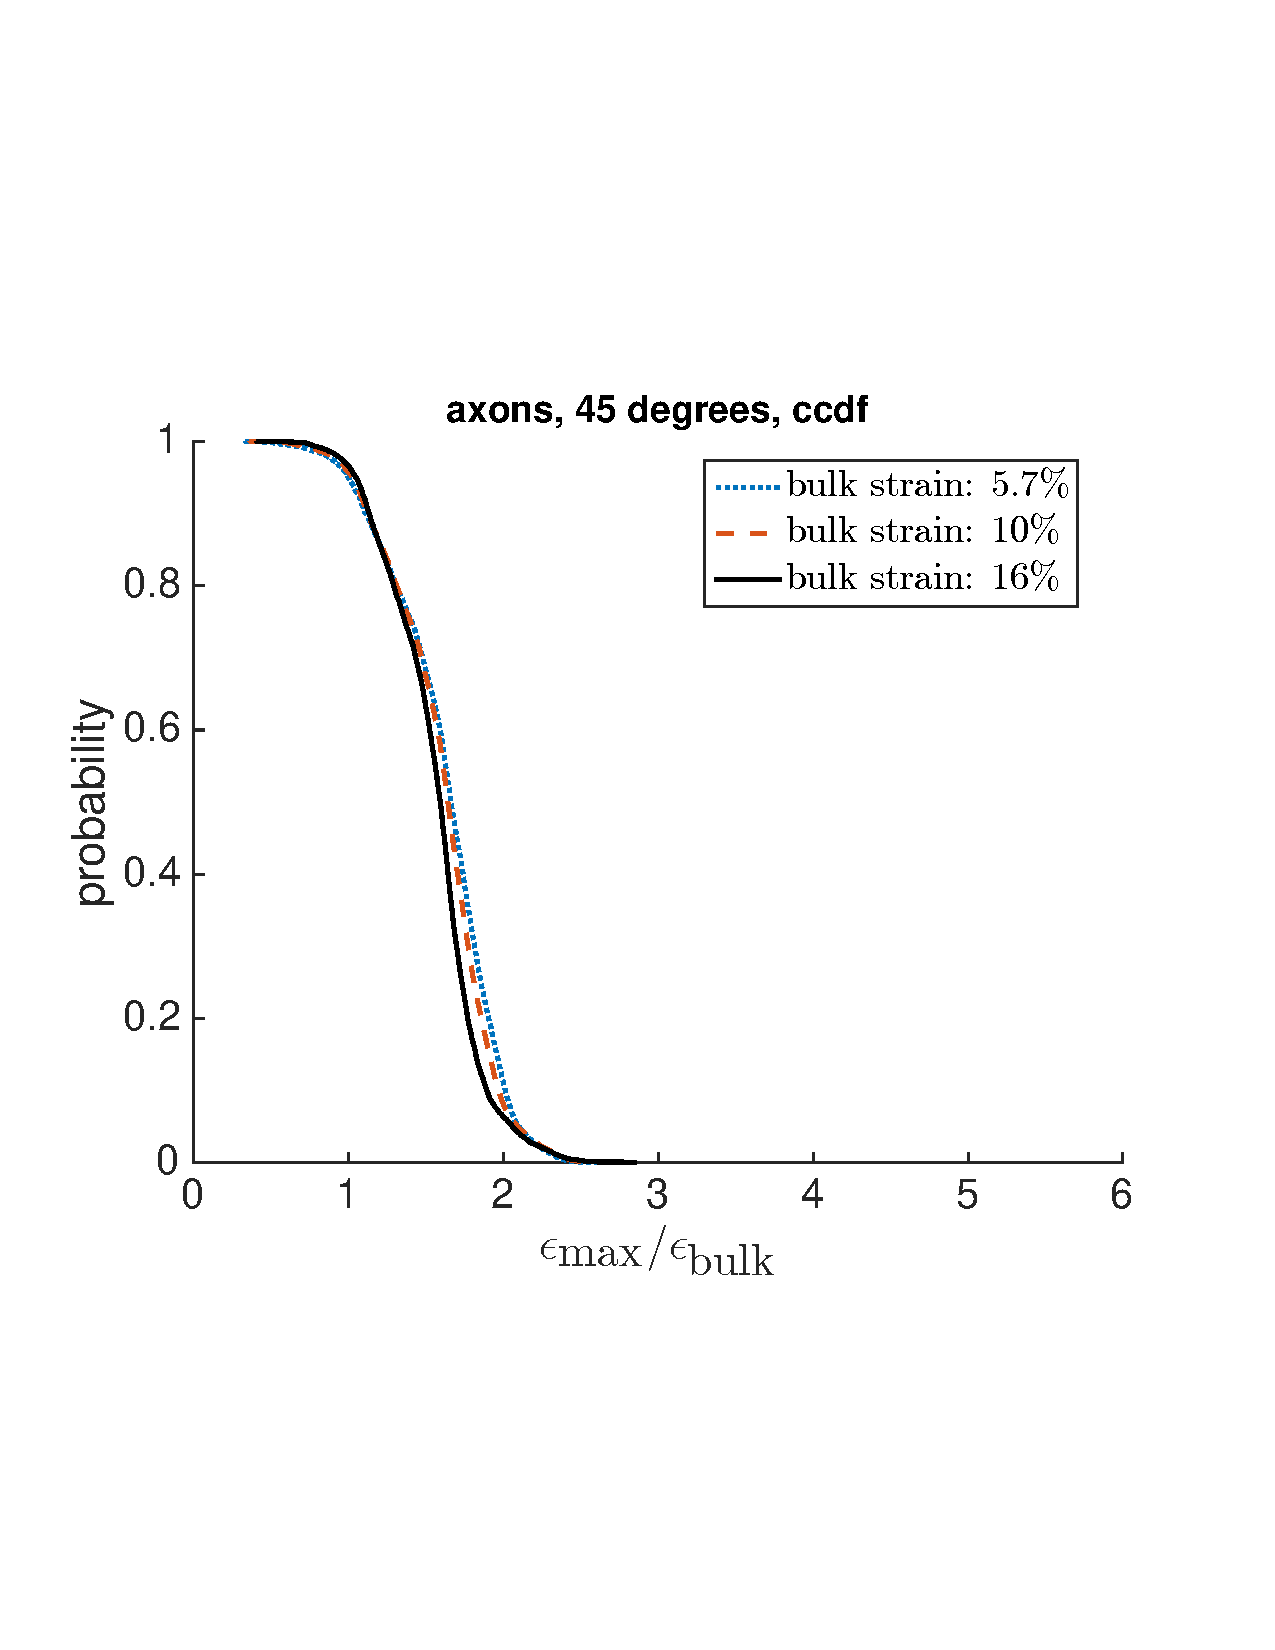
\includegraphics[height=4.5cm]{figure/rot45_FT50_128_1920_ccdf_axons_compare_stps.pdf} &
%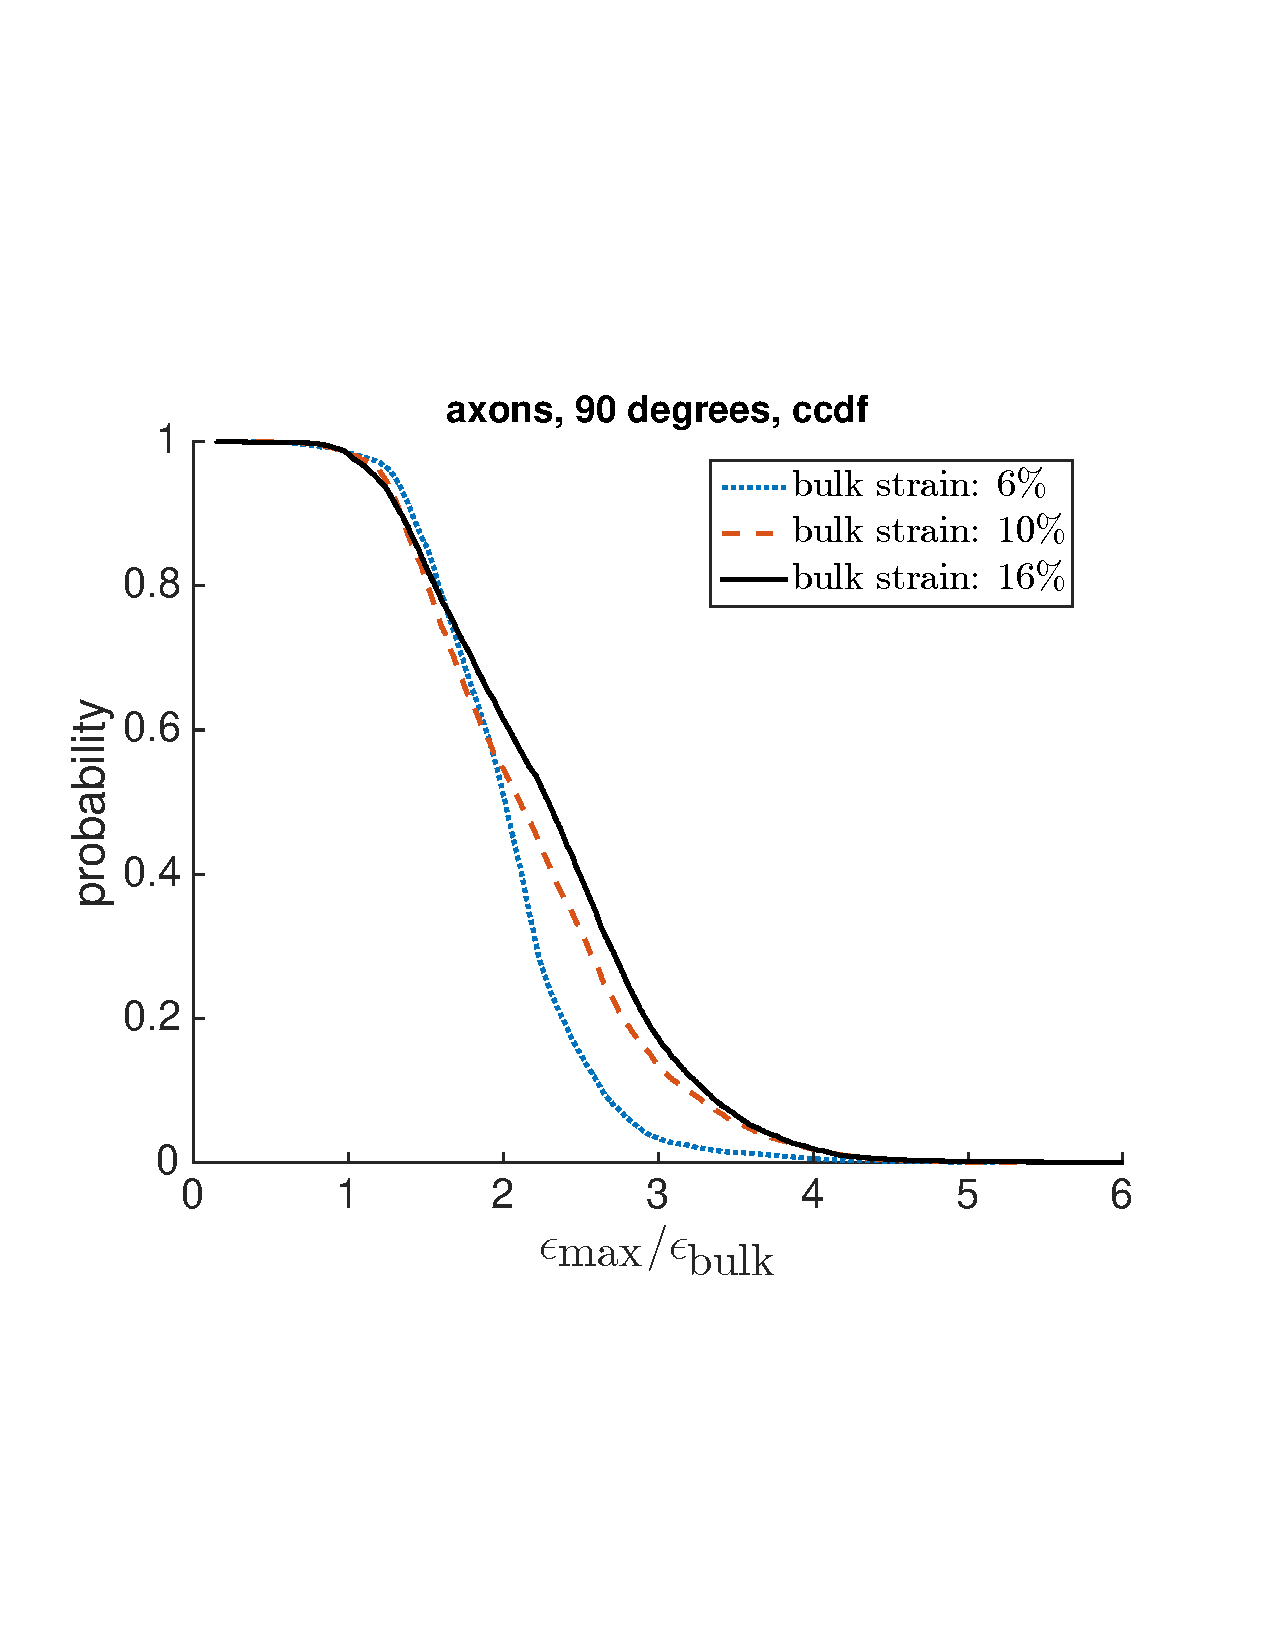
\includegraphics[height=4.5cm]{figure/rot90_FT_dspBC50_a30_128_1920_ccdf_axons_compare_stps_farfield.pdf} \\
%(d) & (e) & (f)
%\end{array}
%$
%\end{center}
%\caption{\label{fig:rgns_ccdf_mps} Distributions of maximum principal strain (ccdf) in the cell bodies (top row) and axons (bottom row) for loading angles of (a,d) 0 degrees, (b,e) 45 degrees, and (c,f) 90 degrees. For each loading angle, distributions for bulk strains of 5 - 6 $\%$ (dotted blue line), 10$\%$ (dashed red line), and 16$\%$ (solid black line) are plotted. The values of $\epsilon_{\text{max}}$ are normalized by the bulk strain, $\epsilon_{\text{bulk}}$.  }
%\end{figure}
%%
%
%The separate distributions for the cell bodies and axons provide additional details about the variations in shape and spread of the neuron distributions in Fig.\ \ref{fig:neuron_ccdf_mps}. For the 0 degree loading case, variations in the distribution at different bulk strains become more apparent. For the cell bodies, the distribution shifts to the right for larger bulk strains indicating that the amplification in the local strain becomes larger with more deformation in the surrounding gel. On the contrary, the middle portion of the axon distribution shifts to the left with increasing bulk strains indicating that the local strain amplification decreases with more deformation in the surrounding gel. The response in the cell bodies and axons cancel out resulting in only slight variations in the overall neuron strain distribution. 
%
%For the 45 degree loading case, variations only arise in the axon distribution. Therefore, the variations seen in the overall neuron distribution is solely due to variations in the axon. Similar to the 0 degree loading case, the axon distribution for the 45 degree loading shifts to the left with larger bulk strains indicating a decrease in the local strain amplification as the surrounding gel is increasingly deformed.
%
%For the 90 degree loading case, large variations are seen in both the cell body and axon distributions. For the cell bodies, the subtle step feature seen in the overall neuron distribution becomes more apparent. This step feature corresponds to two regimes of strain which are clearly seen in the over plot of maximum principal strain on the neuron in Figs.\ \ref{fig:neuron_MPS}(e) and (f). For both the cell body and axon, the distributions shift to the right with increasing bulk strains indicating that the local strain amplification increases with increasing deformation in the surrounding gel. 
%
%The results above indicate that the local strains experienced by the neuron is significantly larger than the applied load on the surrounding gel. The extent of local strain amplification depends on the configuration of the neuron relative to the loading angle. To clarify the cause of local strain amplification in the neuron, the axial strains along a region of the neuron structure are examined.
%
%%=========================================================================================================
%\subsection{Axial Strain Distributions}
%In this section we examine the axial strains, which are more directly linked to the actual geometry of the neuron structure, to shed light on the relationship between local strain amplification and the relative configuration of the neuron with respect to loading angle. Our analysis focuses on a portion of the neuron structure that lies along a single axis. This portion of the neuron is highlighted in Fig.\ \ref{fig:axial_schematic} where the axes on which the strain distributions are calculated are also specified (i.e., axis 1 and axis 2). 
%%
%\begin{figure}[ht]
%\begin{center}
%$
%\begin{array}{c}
%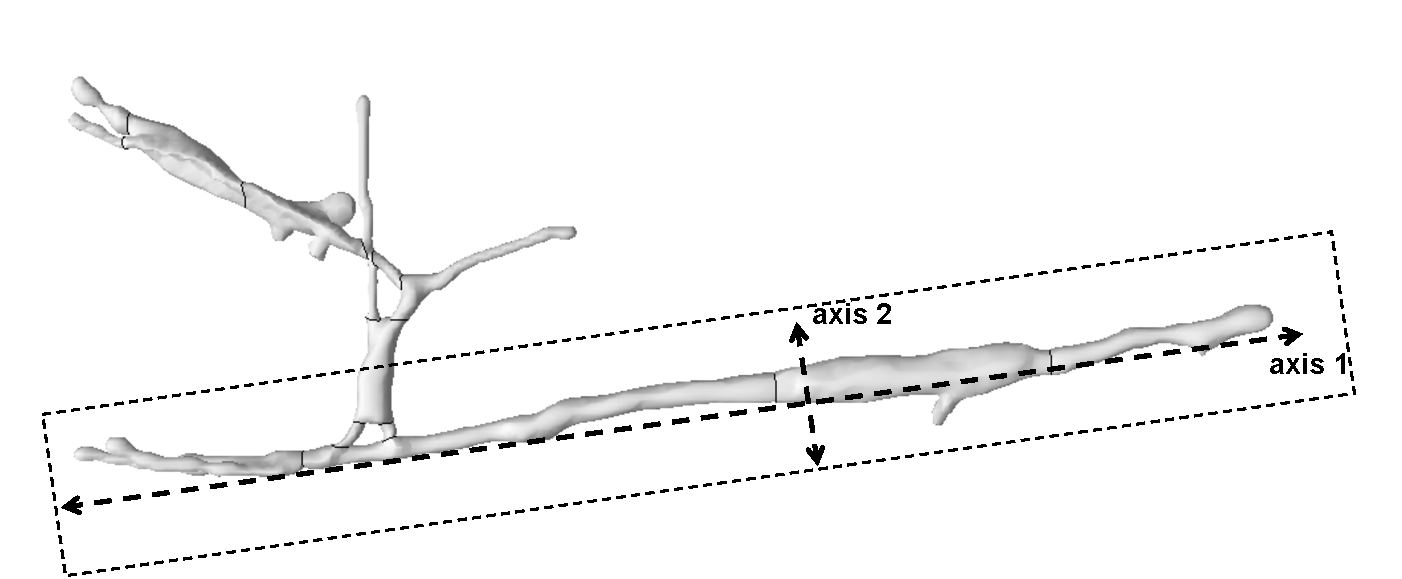
\includegraphics[height=4cm]{figure/axial_coords_schematic.pdf} 
%\end{array}
%$
%\end{center}
%\caption{\label{fig:axial_schematic} Schematic showing the region (rectangular box) and the axes (dashed lines) that are examined.}
%\end{figure}
%%
%
%Distributions of the axial strains along axes 1 and 2 are plotted in Fig.\ \ref{fig:axial_distr} for different loading angles. Depending on the loading angle, axes 1 and 2 will experience either tensile or compressive axial strains. In the case of tensile strains, the ccdf in Eq.\ \eqref{eq:ccdf} is used, while the cdf in Eq.\ \eqref{eq:cdf} is applied for compressive strains. For the 0 degree loading case the axial strains along axis 1 are tensile while those along axis 2 are compressive. The opposite is true for the 90 degree loading case - compressive strain in axis 1 and tensile strain in axis 2 - because the load direction is orthogonal. In the case of 45 degree loading, axis 1 experiences tensile strains while axis 2 experiences mostly compressive strains with a small fraction of the structure experiencing tensile strains.
%%
%% images from N2P178/5-Neuron_LocalAxon_Strain/MaxPrnStrn/PrincipalStranDistr.m
%\begin{figure}[ht]
%\begin{center}
%$
%\begin{array}{ccc}
%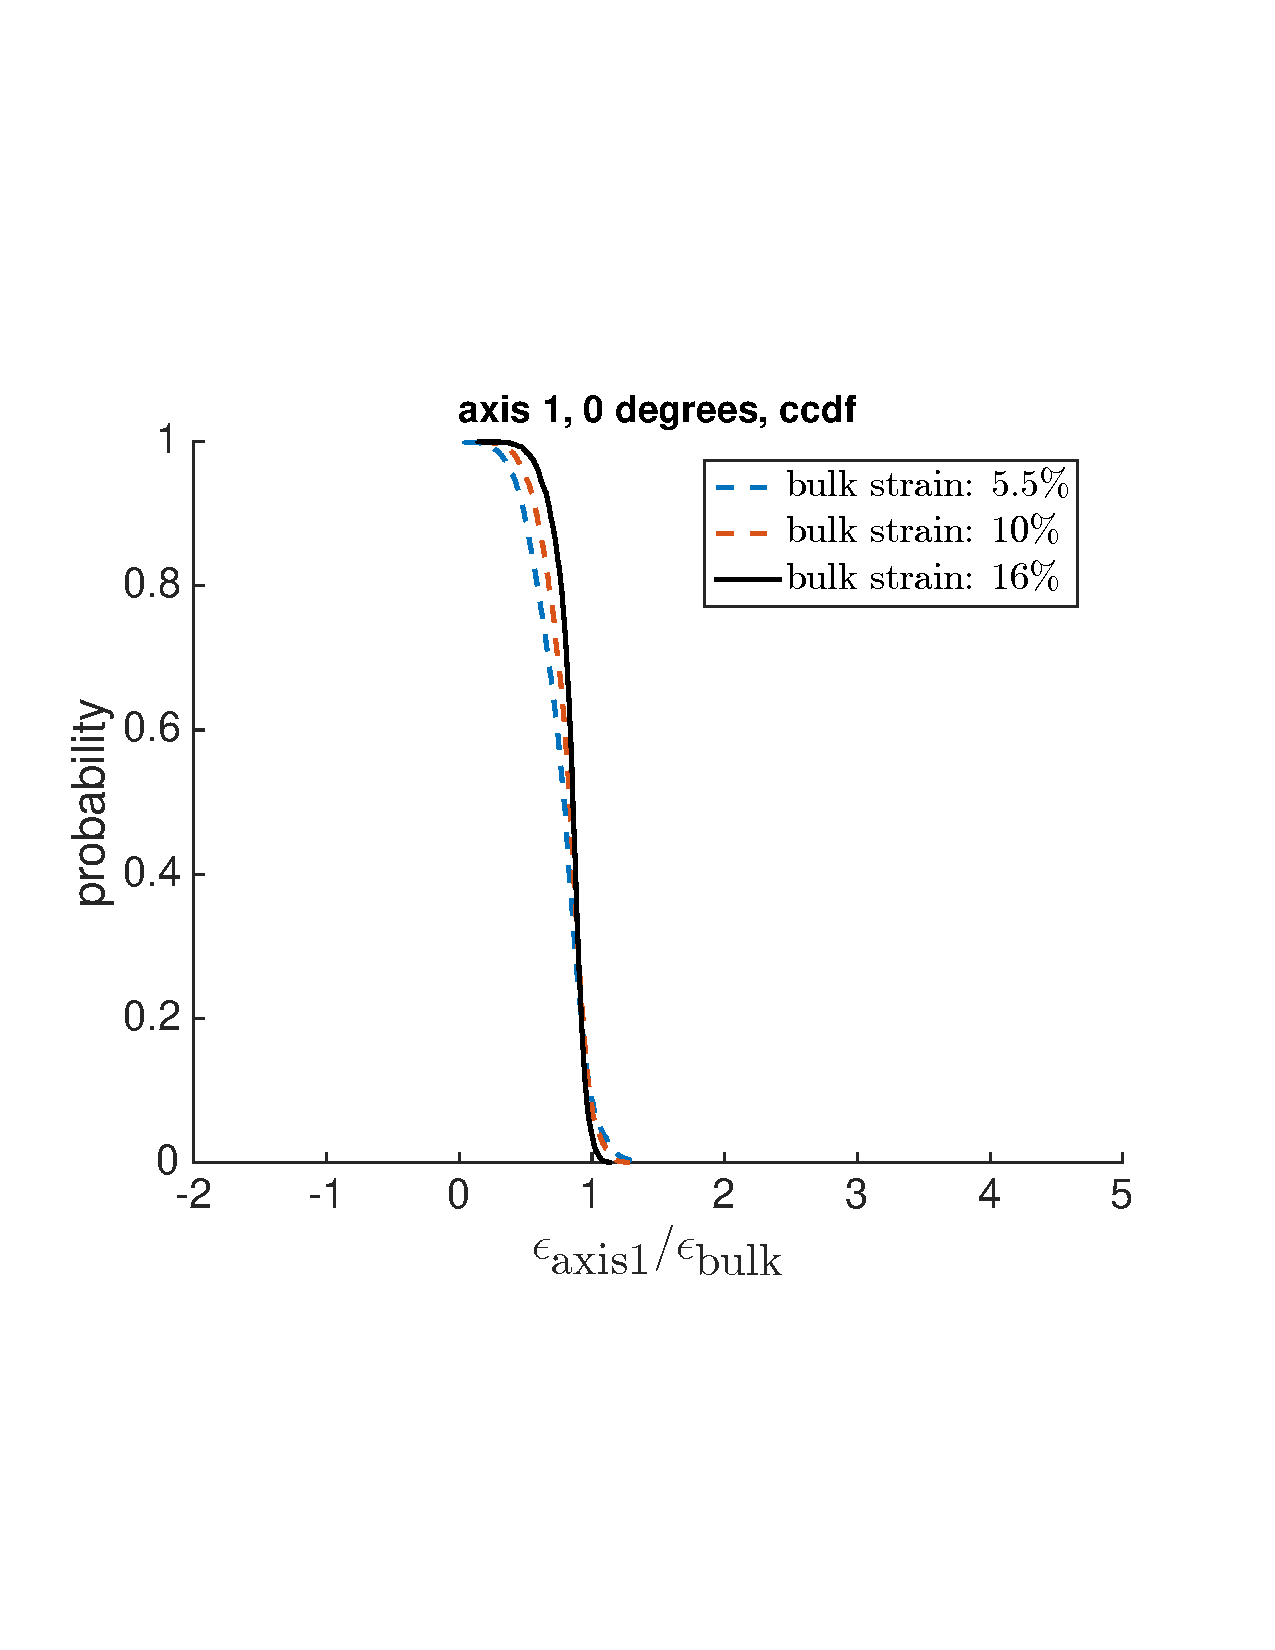
\includegraphics[height=4.5cm]{figure/rot0_FT50_strn11_128_1920_axial_ccdf_axis1_compare_stps.pdf} & 
%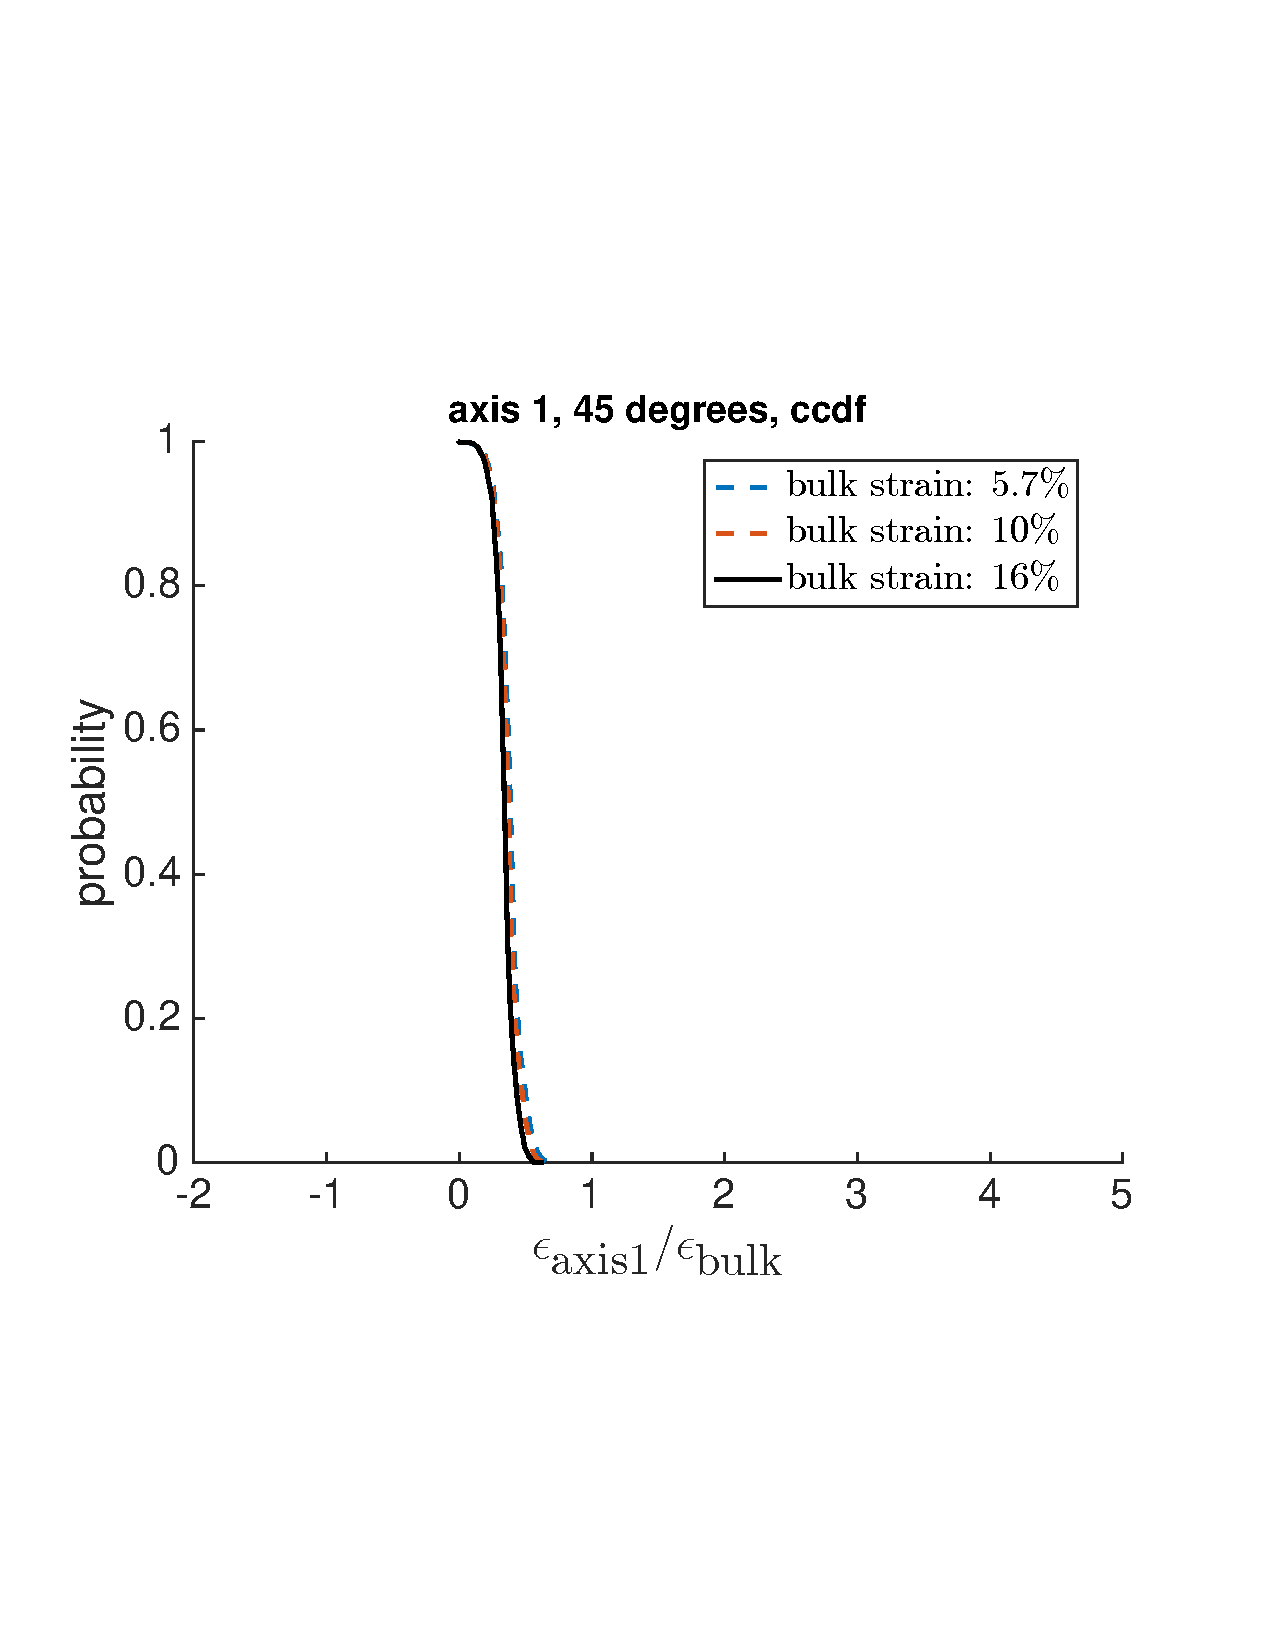
\includegraphics[height=4.5cm]{figure/rot45_FT50_strn11_128_1920_axial_ccdf_axis1_compare_stps.pdf} &
%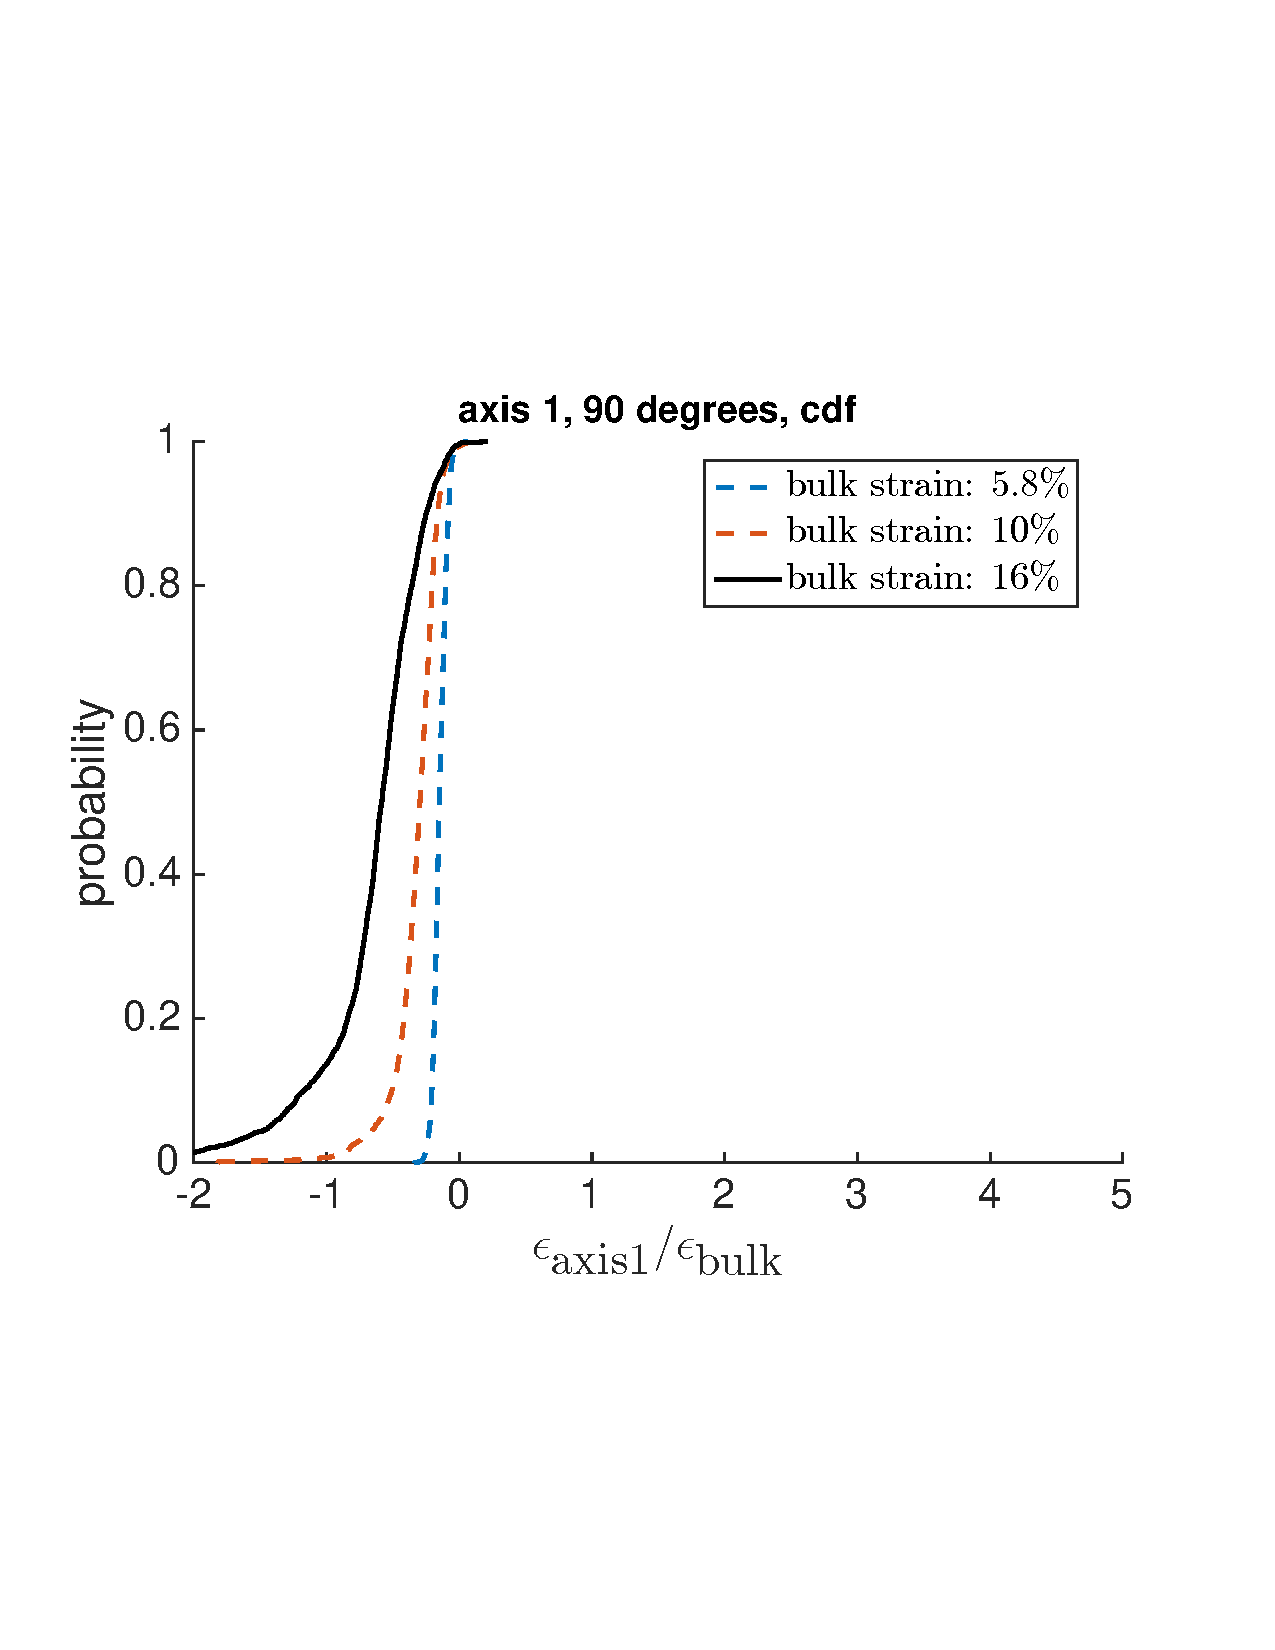
\includegraphics[height=4.5cm]{figure/rot90_FT50_strn11_128_1920_axial_cdf_axis1_compare_stps.pdf} \\
%(a) & (b) & (c) \\ 
%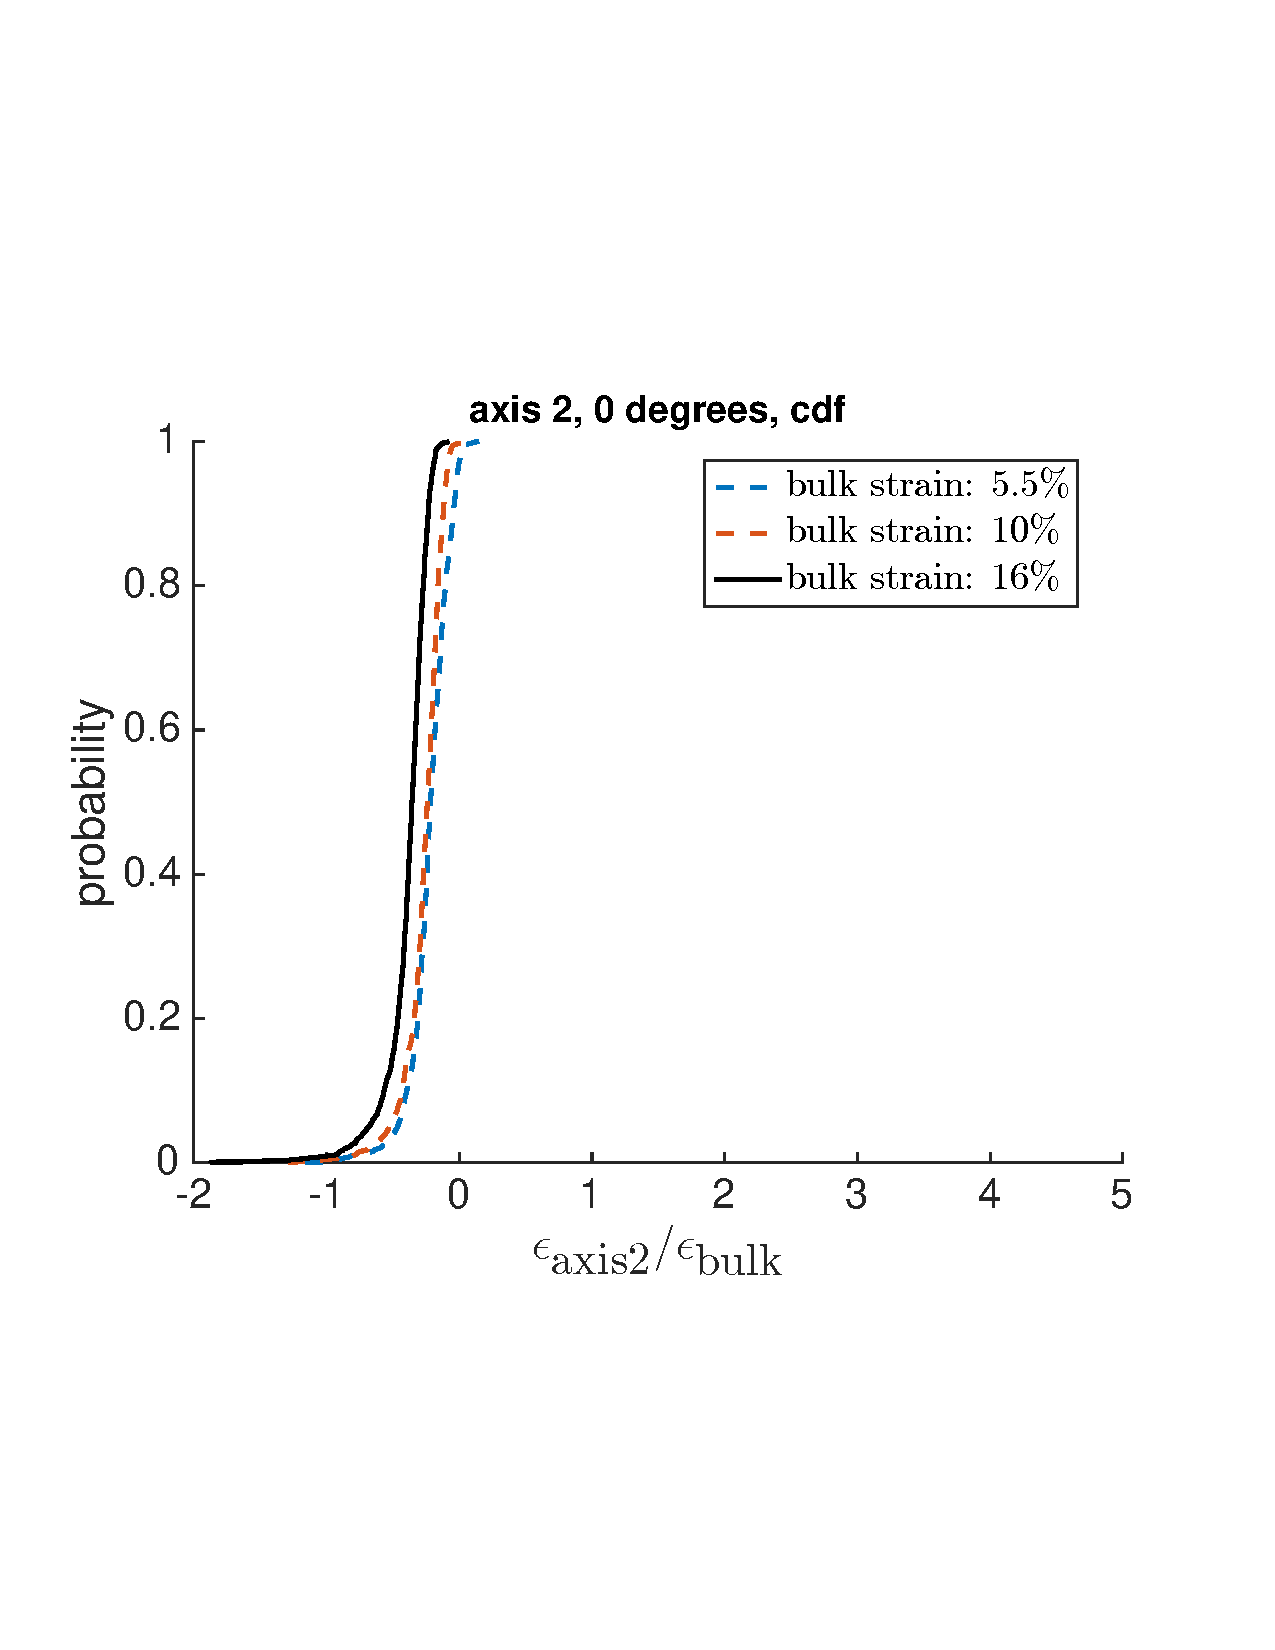
\includegraphics[height=4.5cm]{figure/rot0_FT50_strn22_128_1920_axial_cdf_axis1_compare_stps.pdf} & 
%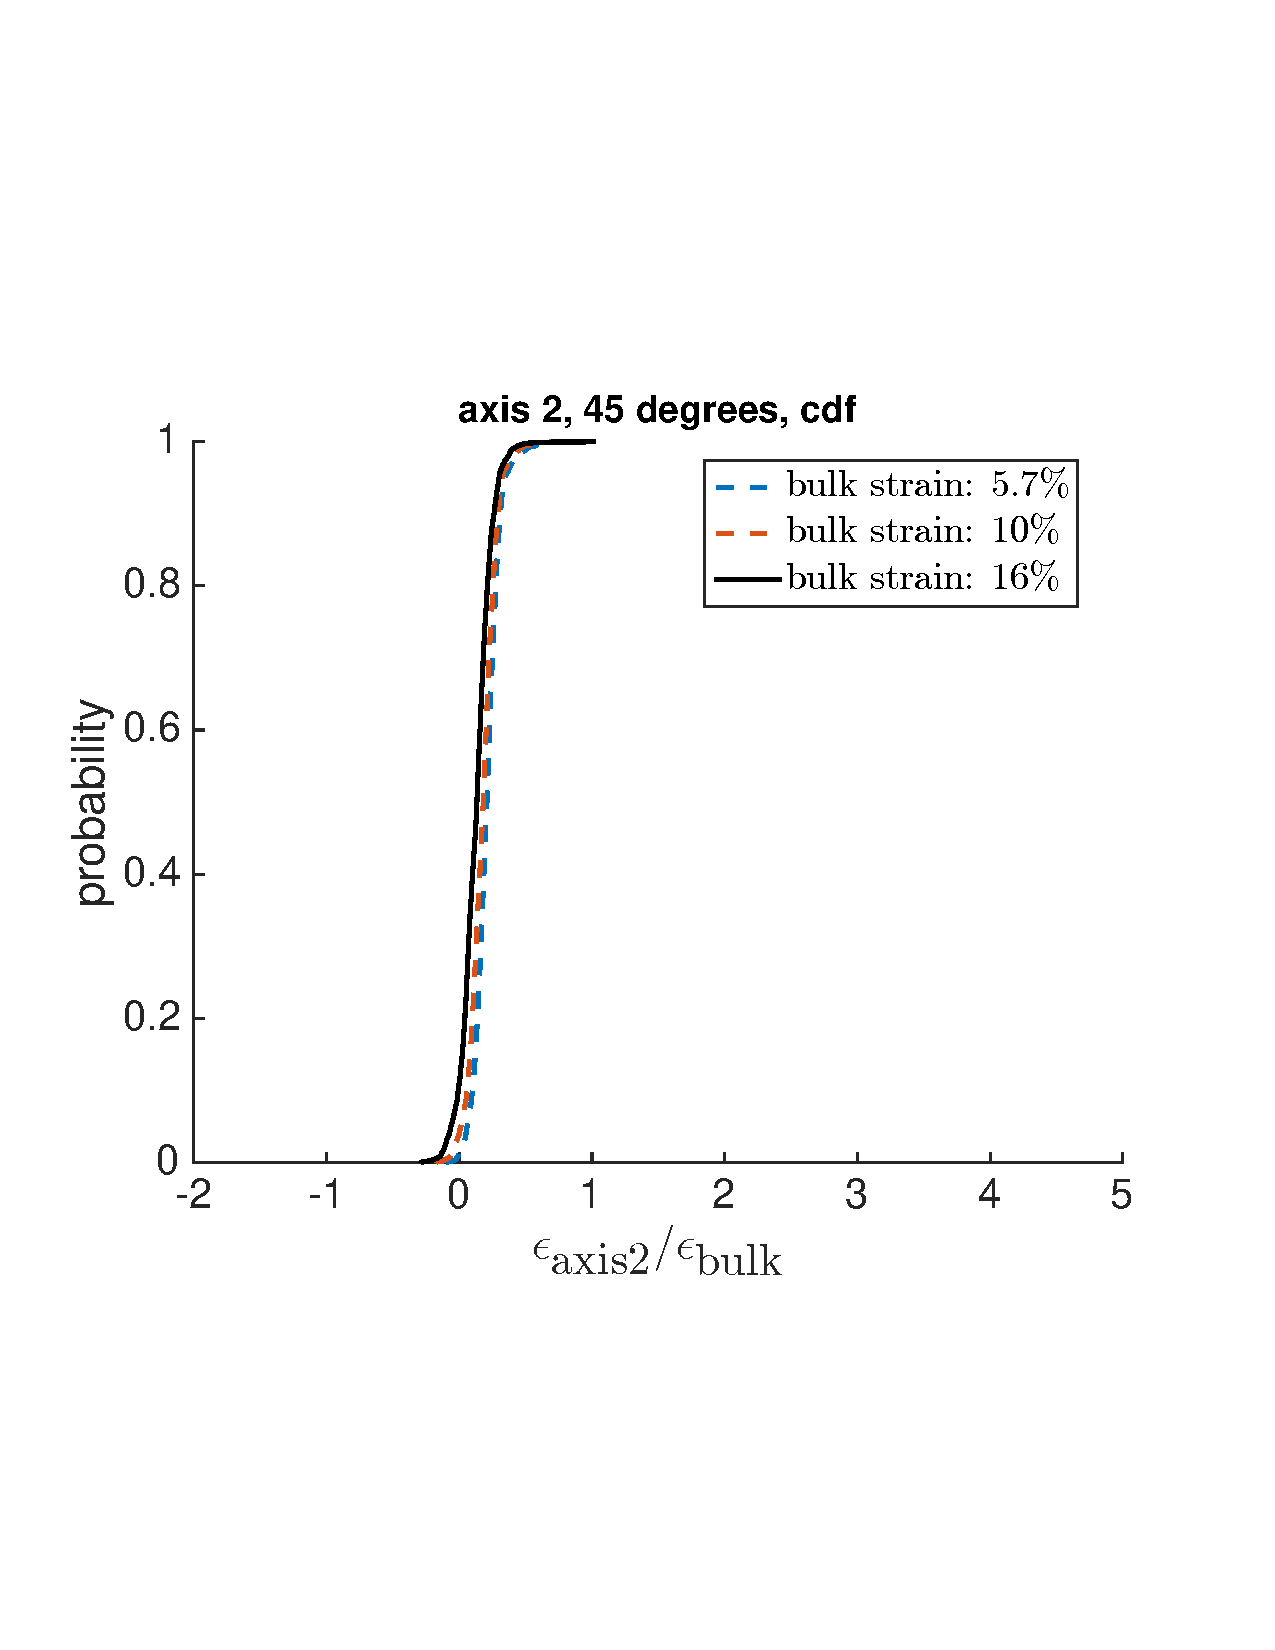
\includegraphics[height=4.5cm]{figure/rot45_FT50_strn22_128_1920_axial_cdf_axis1_compare_stps.pdf} & 
%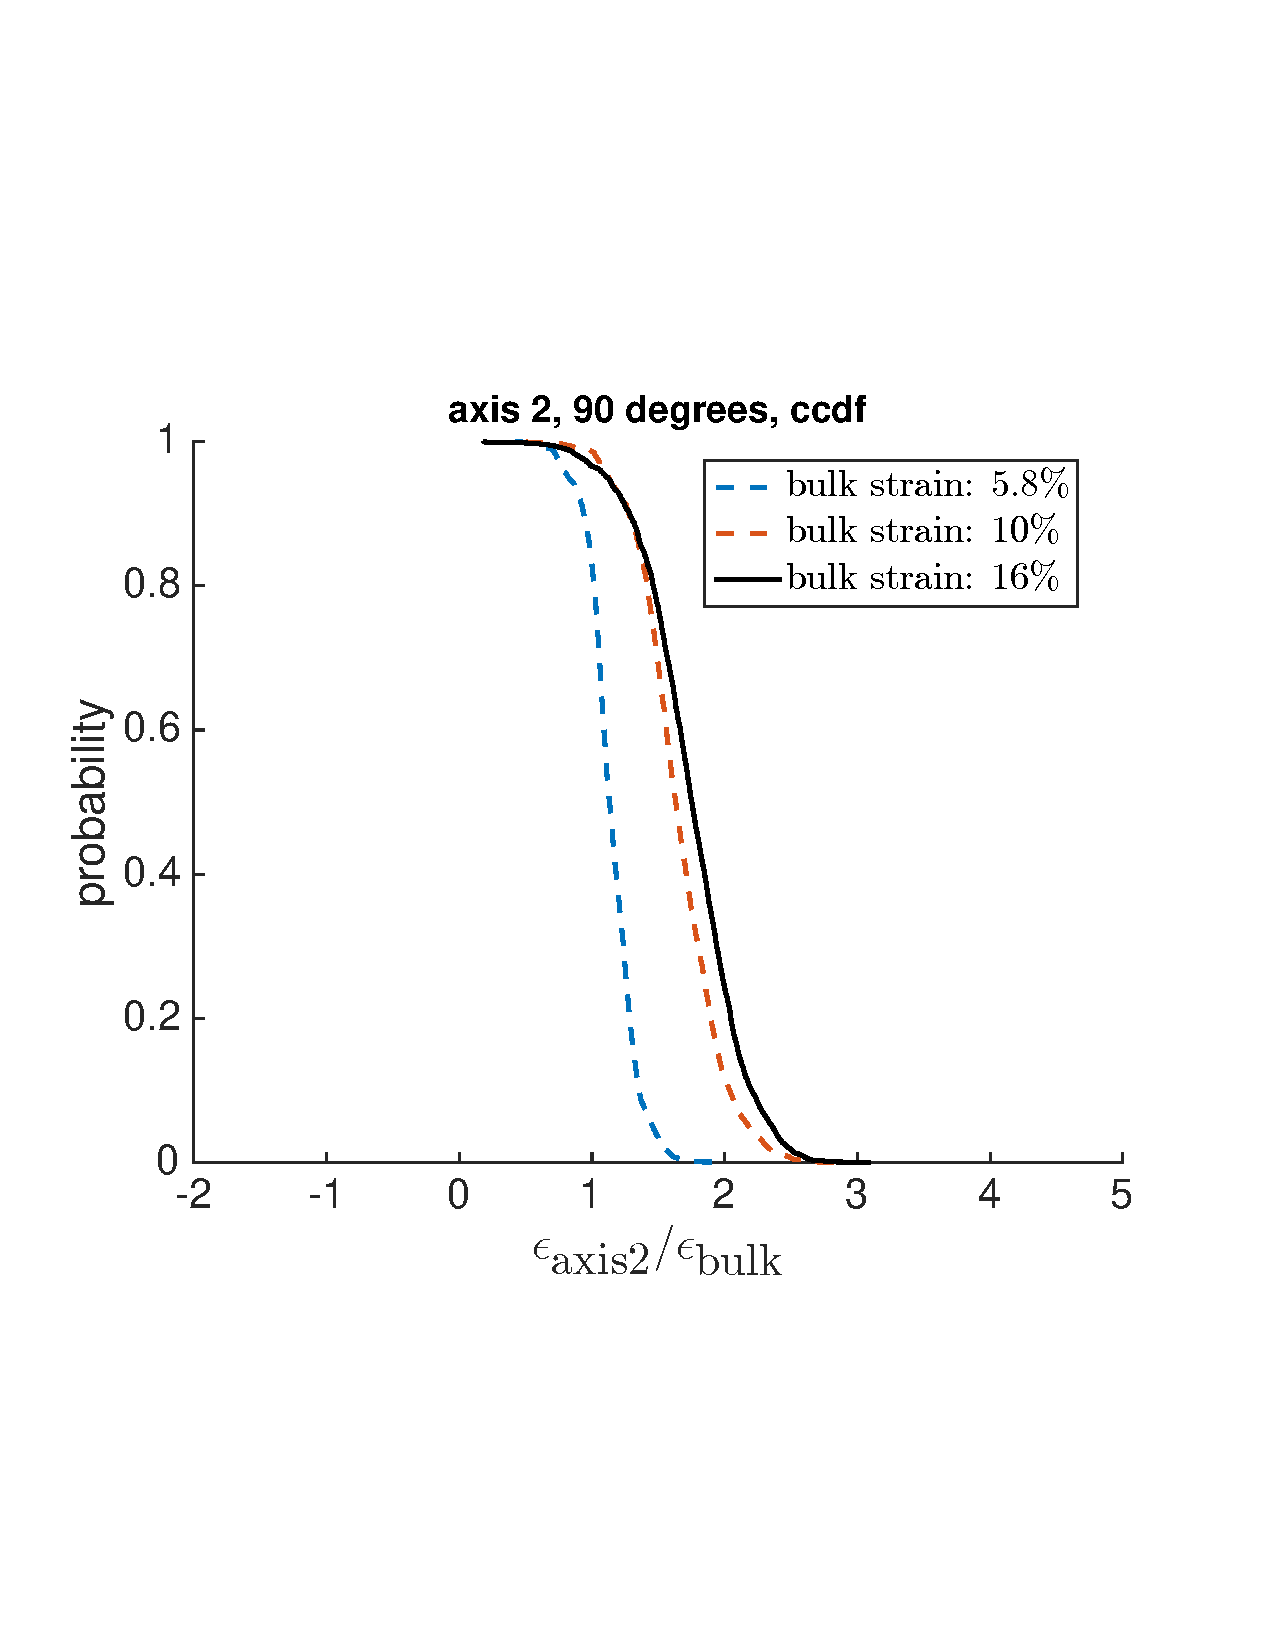
\includegraphics[height=4.5cm]{figure/rot90_FT50_strn22_ptdata_128_1920_axial_ccdf_axis1_compare_stps.pdf} \\
%(d) & (e) & (f) \\
%\end{array}
%$
%\end{center}
%\caption{\label{fig:axial_distr} Distributions of axial strain along axis 1 (top row) and axis 2 (bottom row) for different loading angles. The ccdf is plotted for tensile strains, while the cdf is plotted for compressive strains. For each loading angle, distributions for bulk strains of 5 - 6 $\%$ (dashed blue line), 10$\%$ (dashed red line), and 16$\%$ (solid black line) are plotted. The values of axial strain ($\epsilon_{\text{axis1}}$ or $\epsilon_{\text{axis2}}$) are normalized by the bulk strain, $\epsilon_{\text{bulk}}$.}
%\end{figure}
%%
%
%As seen in Fig.\ \ref{fig:axial_distr}, variations in the strain distributions are greatest for the 90 degree loading case where the amplification of local axial strain increases with increasing bulk strain - the distributions shift left and right for compressive and tensile strains, respectively. In contrast, only small variations are seen in the strain distributions for the 0 and 45 degree loading cases. 
%
%From a physiological stand point, the largest strains (i.e., the tails of the distributions) are most important because those are the regions where neuron damage arises. To understand how the high strain portions of the neuron structure relate to bulk strain applied to the gel, the local-strain amplification corresponding to the portion of the structure that experiences the largest 5$\%$ strain (0.05 on ordinate of distributions in Fig.\ \ref{fig:axial_distr}) are plotted as a function of bulk strain in Fig.\ \ref{fig:axial_amp}. 
%%
%% images are from N2P178/5-Neuron_LocalAxon_Strain/MaxPrnStrn/PlotStrnAmp.m
%\begin{figure}[ht]
%\begin{center}
%$
%\begin{array}{ccc}
%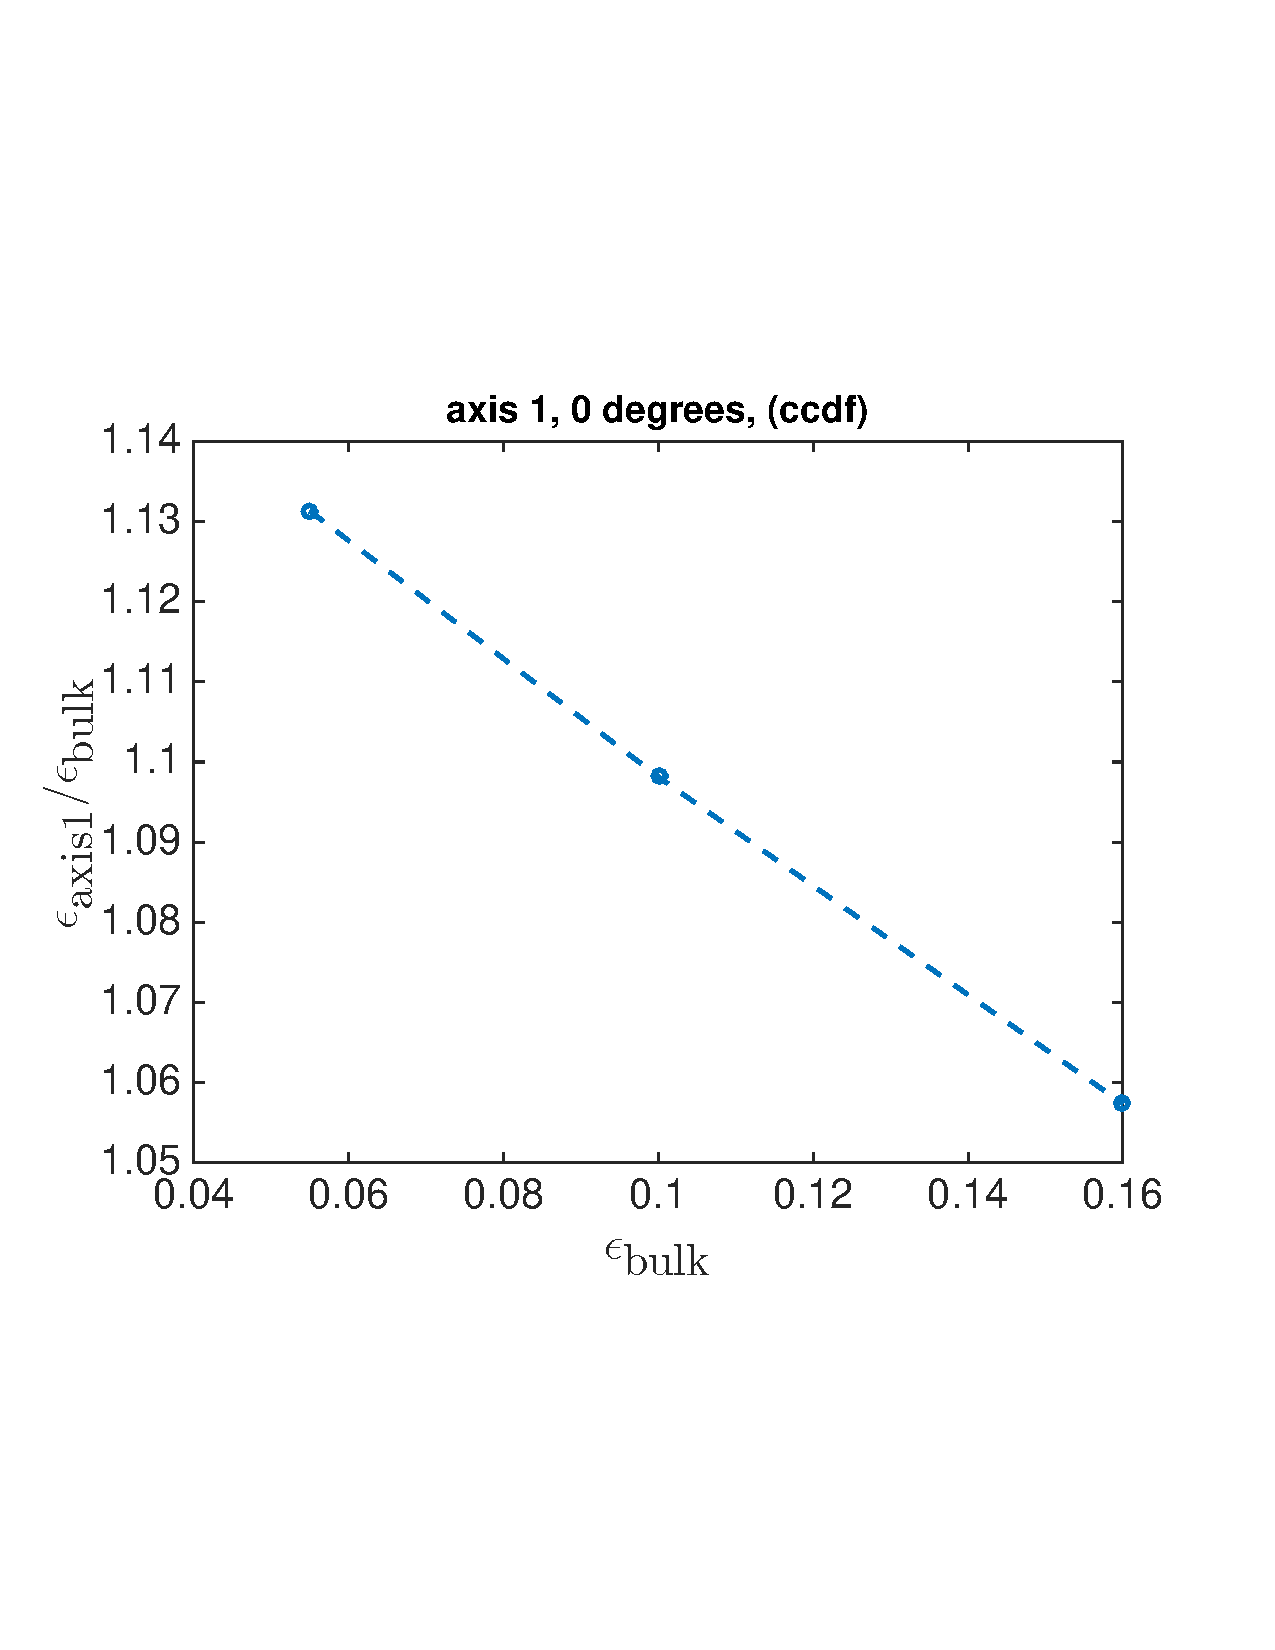
\includegraphics[height=4.5cm]{figure/rot0_FT50_strn11_128_1920_axial_ccdf_axis1_strn_amp.pdf} & 
%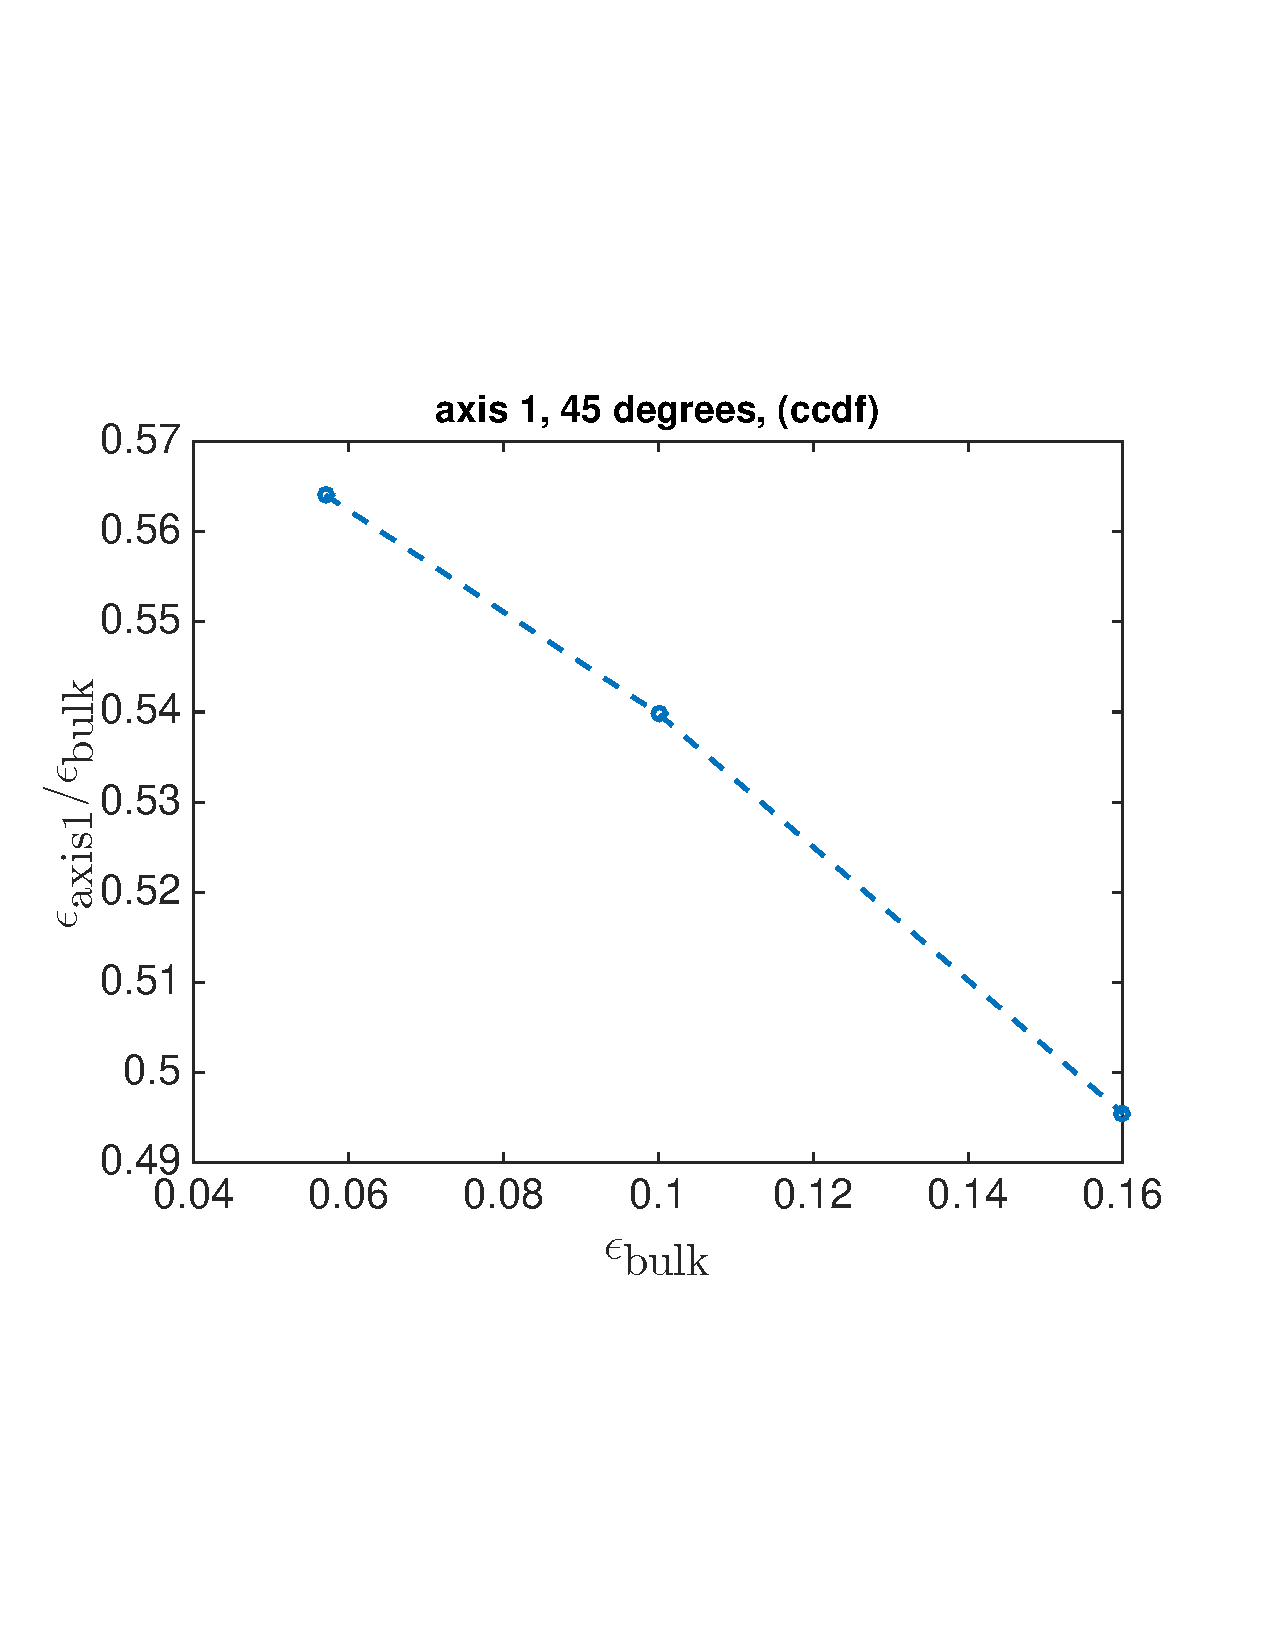
\includegraphics[height=4.5cm]{figure/rot45_FT50_strn11_128_1920_axial_ccdf_axis1_strn_amp.pdf} &
%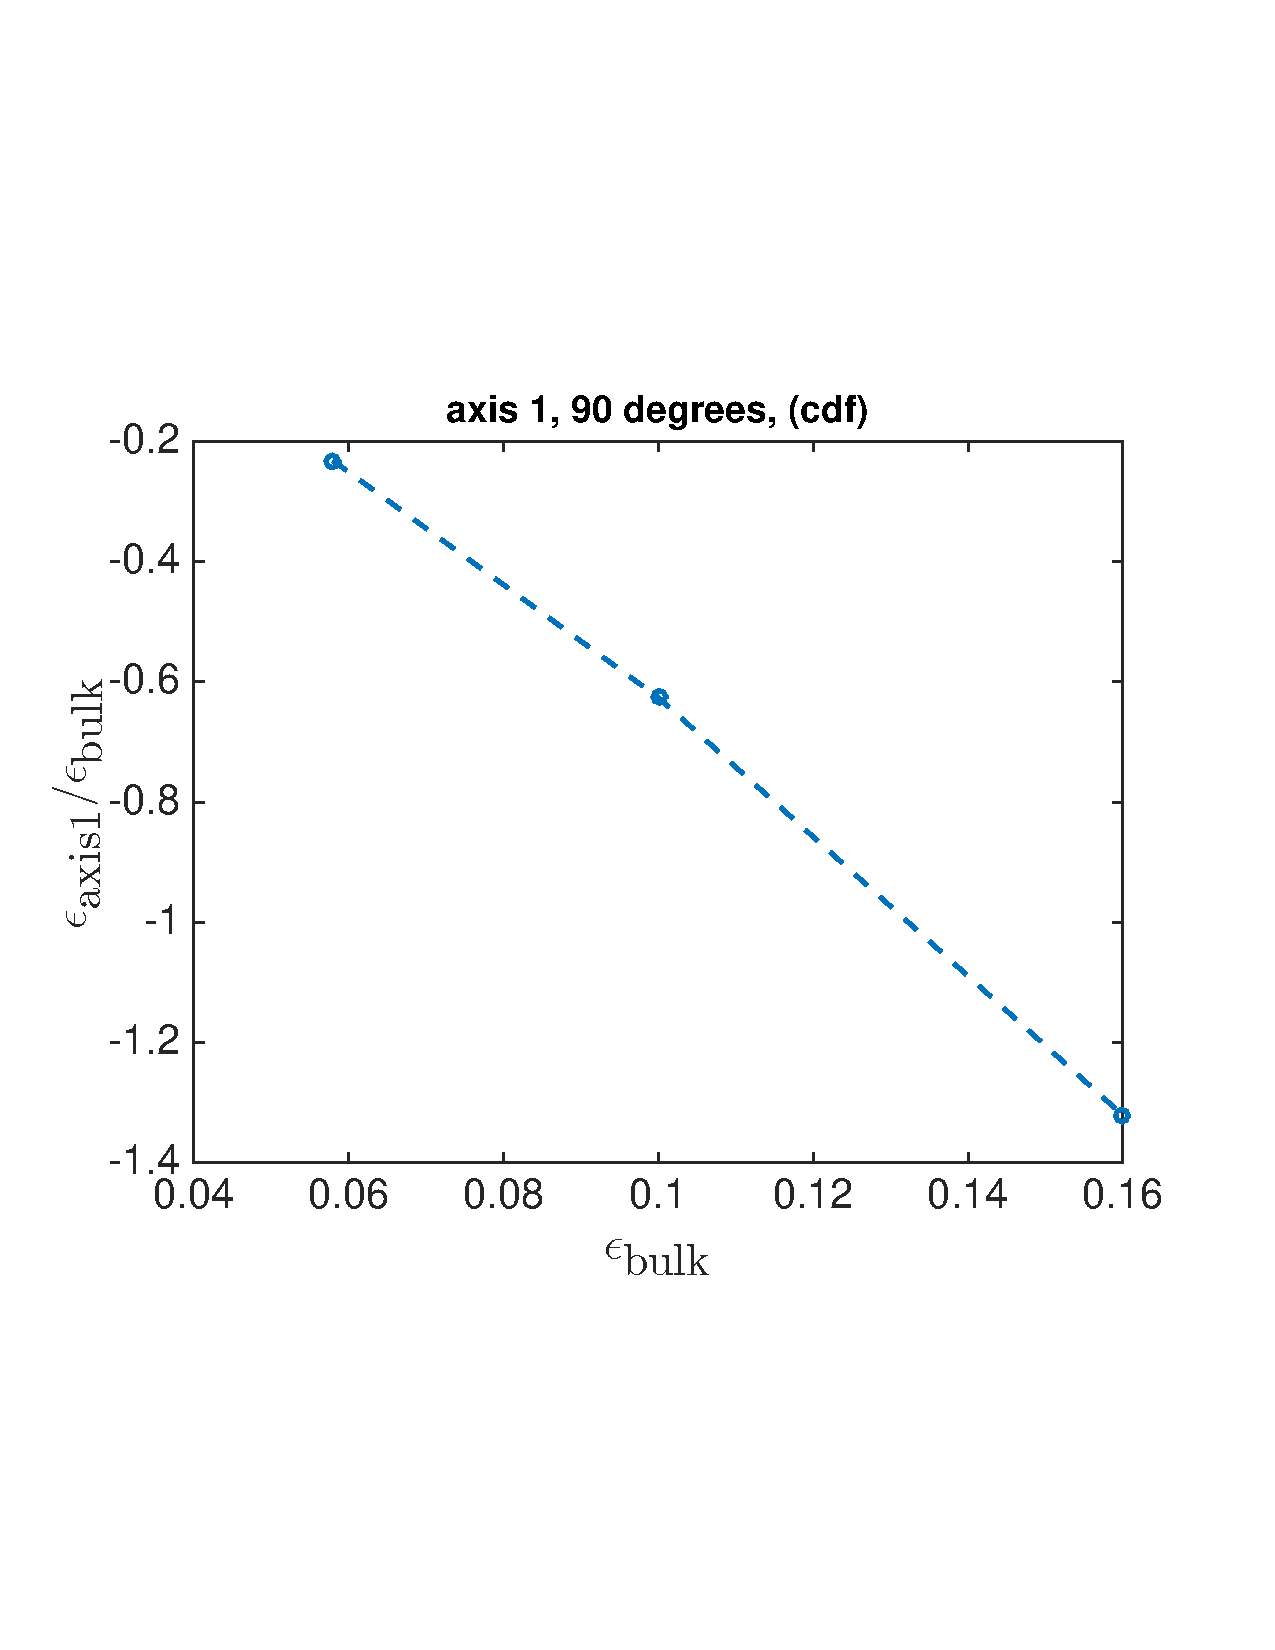
\includegraphics[height=4.5cm]{figure/rot90_FT50_strn11_128_1920_axial_cdf_axis1_strn_amp.pdf} \\
%(a) & (b) & (c) \\ 
%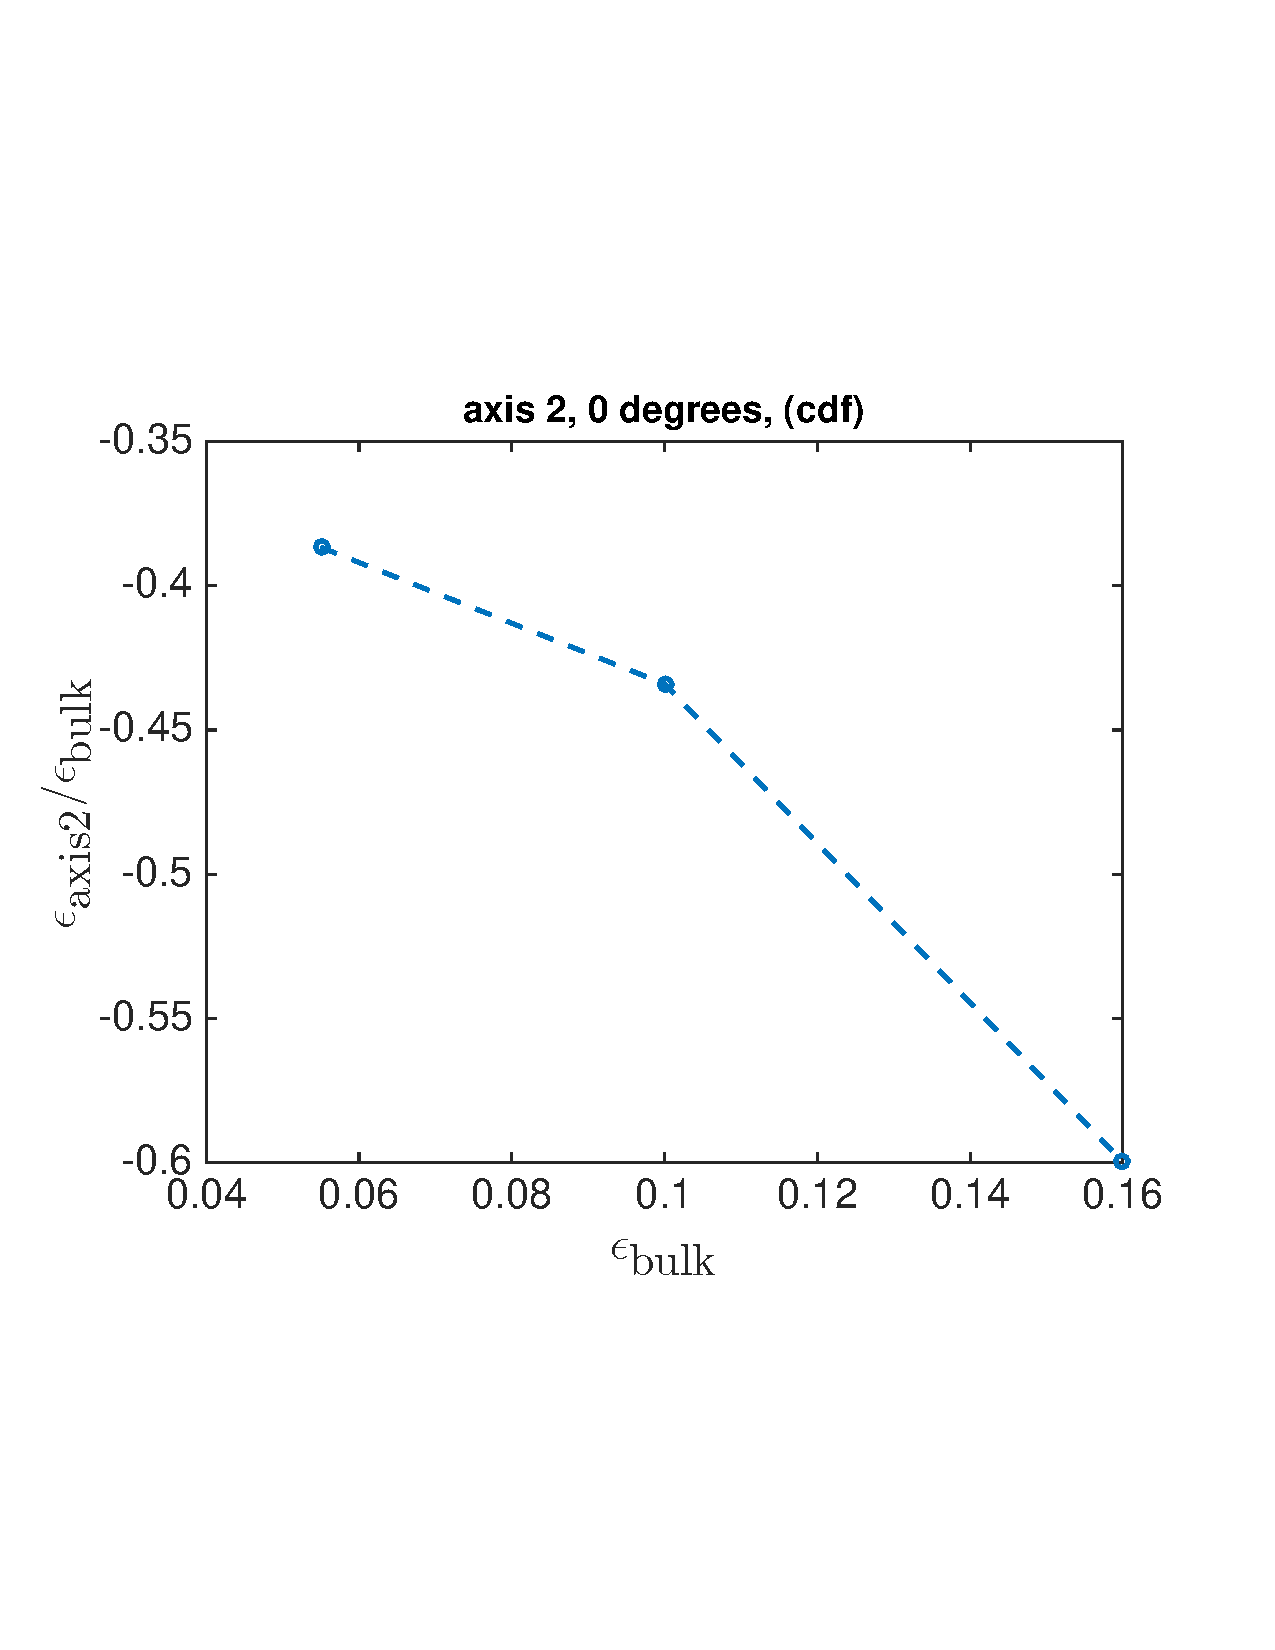
\includegraphics[height=4.5cm]{figure/rot0_FT50_strn22_128_1920_axial_cdf_axis1_strn_amp.pdf} &
%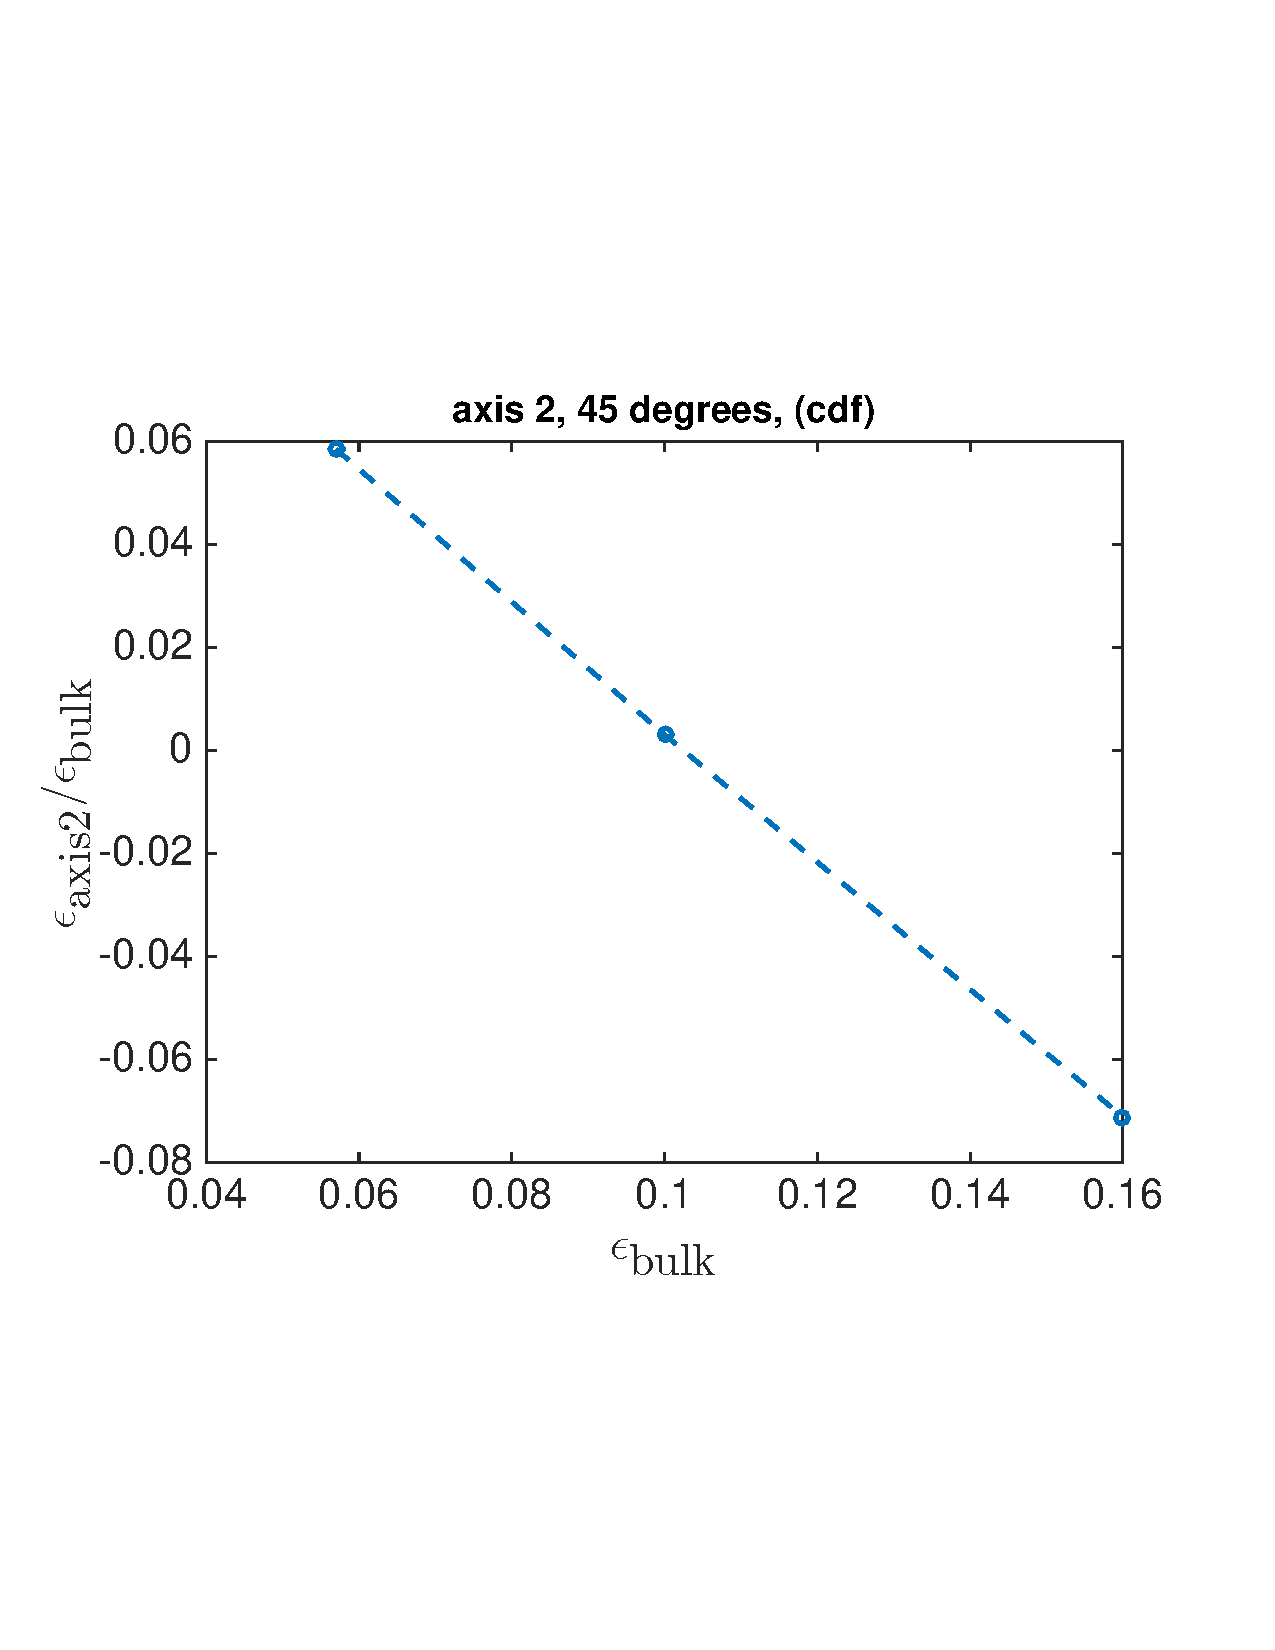
\includegraphics[height=4.5cm]{figure/rot45_FT50_strn22_128_1920_axial_cdf_axis1_strn_amp.pdf} & 
%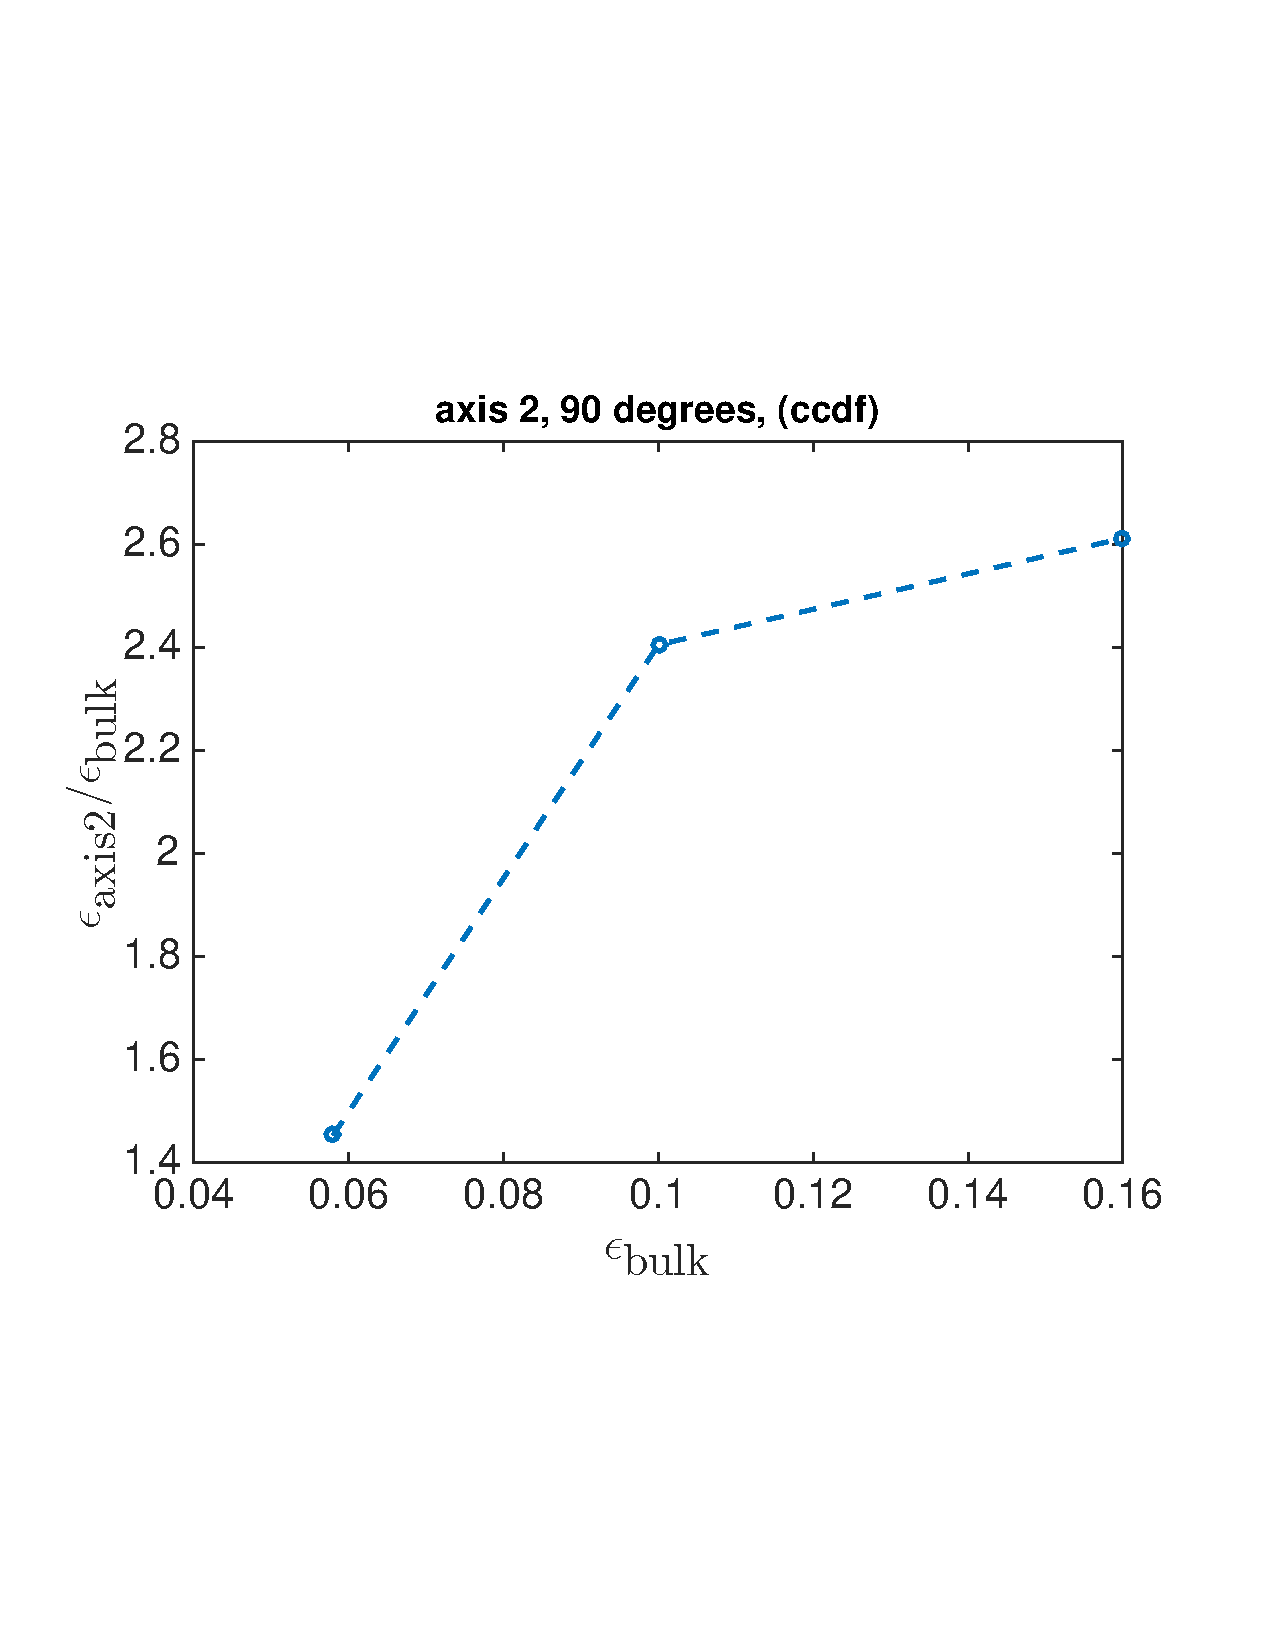
\includegraphics[height=4.5cm]{figure/rot90_FT50_strn22_128_1920_axial_ccdf_axis1_strn_amp.pdf} \\
%(d) & (e) & (f) 
%\end{array}
%$
%\end{center}
%\caption{\label{fig:axial_amp} Local strain amplification corresponding to the portion of the neuron structure in Fig.\ \ref{fig:axial_schematic} that experiences the largest 5$\%$ strain (0.05 on ordinate of distributions in Fig.\ \ref{fig:axial_distr}) as a function of bulk strain for different loading directions.}
%\end{figure}
%%
%
%As seen in Fig.\ \ref{fig:axial_amp}, the local-strain amplification of the lateral compressive strains increase for all loading angles - axis 2 for 0 and 45 degree loading and axis 1 for 90 degree loading. This is consistent with the fact that the Poisson ratio of the collagen gel increases with larger deformations (see Poisson ratio curve in Fig.\ \ref{fig:fiber_param2}(a)). Note that for 45 degree loading, axis 2 experiences tensile strains at smaller bulk strains before the lateral compressive strains that arise from the Poisson ratio effect become large enough to dominate. Interestingly, the local-strain amplification of the tensile strain decreases for the 0 and 45 degree loading cases and increases for the 90 degree loading cases - axis 1 for 0 and 45 degree loading and axis 2 for 90 degree loading. This result suggests that a configuration where the axial direction of the neuron is near parallel to the loading direction (e.g., axis 1 for 0 and 45 degree loading cases) is more favorable than a configuration where the axial direction of the neuron is near orthogonal to the loading direction (e.g., axis 2 for the 90 degree loading case). The underlying mechanisms for such behavior is explored in the next section.

%%%%%%%%%%%%%%%%%%%%%%%%%%%%%%%%%%%%%%%%%%%%%%%%%%%%%%%%%%%%%%%%%%%%%%
\section{Discussion}
\label{sec:discussion}
The results in Sections \ref{sec:cellbody_stiffness} and \ref{sec:loading_direction} illustrate that the strain distribution (ccdf) in the neuron structure, and hence strain amplification, is most strongly influenced by the configuration of the neuron with respect to the loading direction. The strong dependence of the strain distribution on loading configuration reflects the anisotropic nature of the embedded neuron structure, where the axial stiffness is one order of magnitude stiffer than the transverse stiffness. Relative to the stiffness of the surrounding collagen gel, the axial stiffness of the neuron is larger while the transverse stiffness of the neuron is smaller. Due to the complex geometry of the embedded neuron structure studied above, the neuron structure is exposed to both transverse and axial components of loading. The spread of ccdfs reflects the range of tranverse and axial loads that different regions within the neuron structure is exposed to.

Some insight about the magnitude of the strain amplification for transverse and axial loading can be gained by simplifying the embedded neuron structure system into a one-dimensional gel-neuron-gel series configuration. For such a system, the strain in the neuron can be expressed in terms of the strain in the gel by
%
\begin{equation}
\epsilon_{\text{neuron}} = \frac{K_{\text{gel}}}{K_{\text{neuron}}}\epsilon_{\text{gel}},
\label{eq:series_analysis}
\end{equation}
%
where $K_{\text{gel}}$ and $K_{\text{neuron}}$ are the stiffnesses in the gel and neuron, respectively. The ratio of gel stiffness to neuron stiffness represents the strain amplification in the neuron structure. The simplified series configuration represents an upper bound for the strain amplification experienced in the neuron structure. Using Eq.\ \ref{eq:series_analysis}, the upper bounds of the two extremes of pure transverse and axial loading can be examined. 

At one extreme when the load on the neuron structure is purely transverse, $K_{\text{neuron}} = 1.5$ kPa and is less than $K_{\text{gel}}$. Since $K_{\text{neuron}} < K_{\text{gel}}$, strain amplification in the neuron structure arises. The strain amplification becomes larger with deformation because the $K_{\text{gel}}$ increases due to stiffening during deformation. From Eq.\ \eqref{eq:series_analysis}, the strain amplification for non painful and painful loading is 17.8 and 31.6 times, respectively.

At the other extreme when the load on the neuron structure is purely axial, $K_{\text{neuron}} = 70$ kPa and is greater than $K_{\text{gel}}$. Since $K_{\text{neuron}} > K_{\text{gel}}$, the strain experienced by the neuron structure is less than that in the gel. The strain discrepancy between the neuron structure and gel decreases with deformation due to the stiffening of the collagen gel. From Eq.\ \eqref{eq:series_analysis}, the strain amplification for non painful and painful loading is 0.38 and 0.68 times, respectively.

The upper bound scenarios described above can be applied to understand the simulation results for the embedded neuron structure. In all cases of non painful and painful ligament loading considered, the average strain amplification is greater than one. This suggests that on average the neuron structure is exposed to more transverse loading than axial loading. As the loading angle varies from 0 to 90 degrees, the volume fraction of neuron that is exposed to transverse loading increases as reflected by the increasing average strain amplification.

As mentioned above, the spread in the strain distributions reflect the complex geometry of the neuron structure. Of the three loading angles considered, the neuron structure is loaded most uniformly at 45 degrees as reflected by the relatively narrow spread of its strain distribution. The wider spread in the strain distributions for 0 and 90 degree loading is due to the existence of neurons in the structure that lie nearly parallel to the 0 degree and 90 degree axis. As a result, when the gel is loaded at either 0 or 90 degrees, the neuron structure will be exposed to both extremes of nearly pure transverse and axial loadings. 

Physiologically most important is the right tail of the distributions, which corresponds to the maximum strain experienced in the neuron structure. Of the cases considered, the largest strain amplification in the neuron structure is observed when the gel is loaded at 90 degrees. As seen in Table \ref{table:ccdf_volfrac_compare}, 9.7$\%$ and 14$\%$ of the neuron structure experiences a three times or more strain amplification for non painful and painful ligament loading, respectively. In comparison,  0.2$\%$  and 0$\%$ of the neuron structure experiences a three times or more strain amplification for 0 and 45 degree loading, respectively. The volume fraction that experiences a two times or more strain amplification for the 0 and 45 degree loading cases is still less than the volume fraction experiencing three times or more strain amplification in the 90 degree loading case.

Of the three loading configurations considered, the 90 degree loading case is most susceptible to neuronal damage during ligament loading as reflected by the large average and long tail of its distribution. In the cases of the 0 and 45 degree loading, the strain distribution for 45 degrees has a larger average while that for 0 degrees has a longer tail. Therefore, whether the 0 or 45 degree loading case is more susceptible to neuron injury depends on the damage threshold of the neuron. For example, if the damage threshold for the neuron is three times the applied load on the gel, then the 0 degree loading case will be more susceptible to neuronal damage due to the longer tail in its distribution.


%\subsection{Fiber Alignment in Collagen Gel}
%%
%\begin{figure}[ht]
%\begin{center}
%$
%\begin{array}{ccc}
%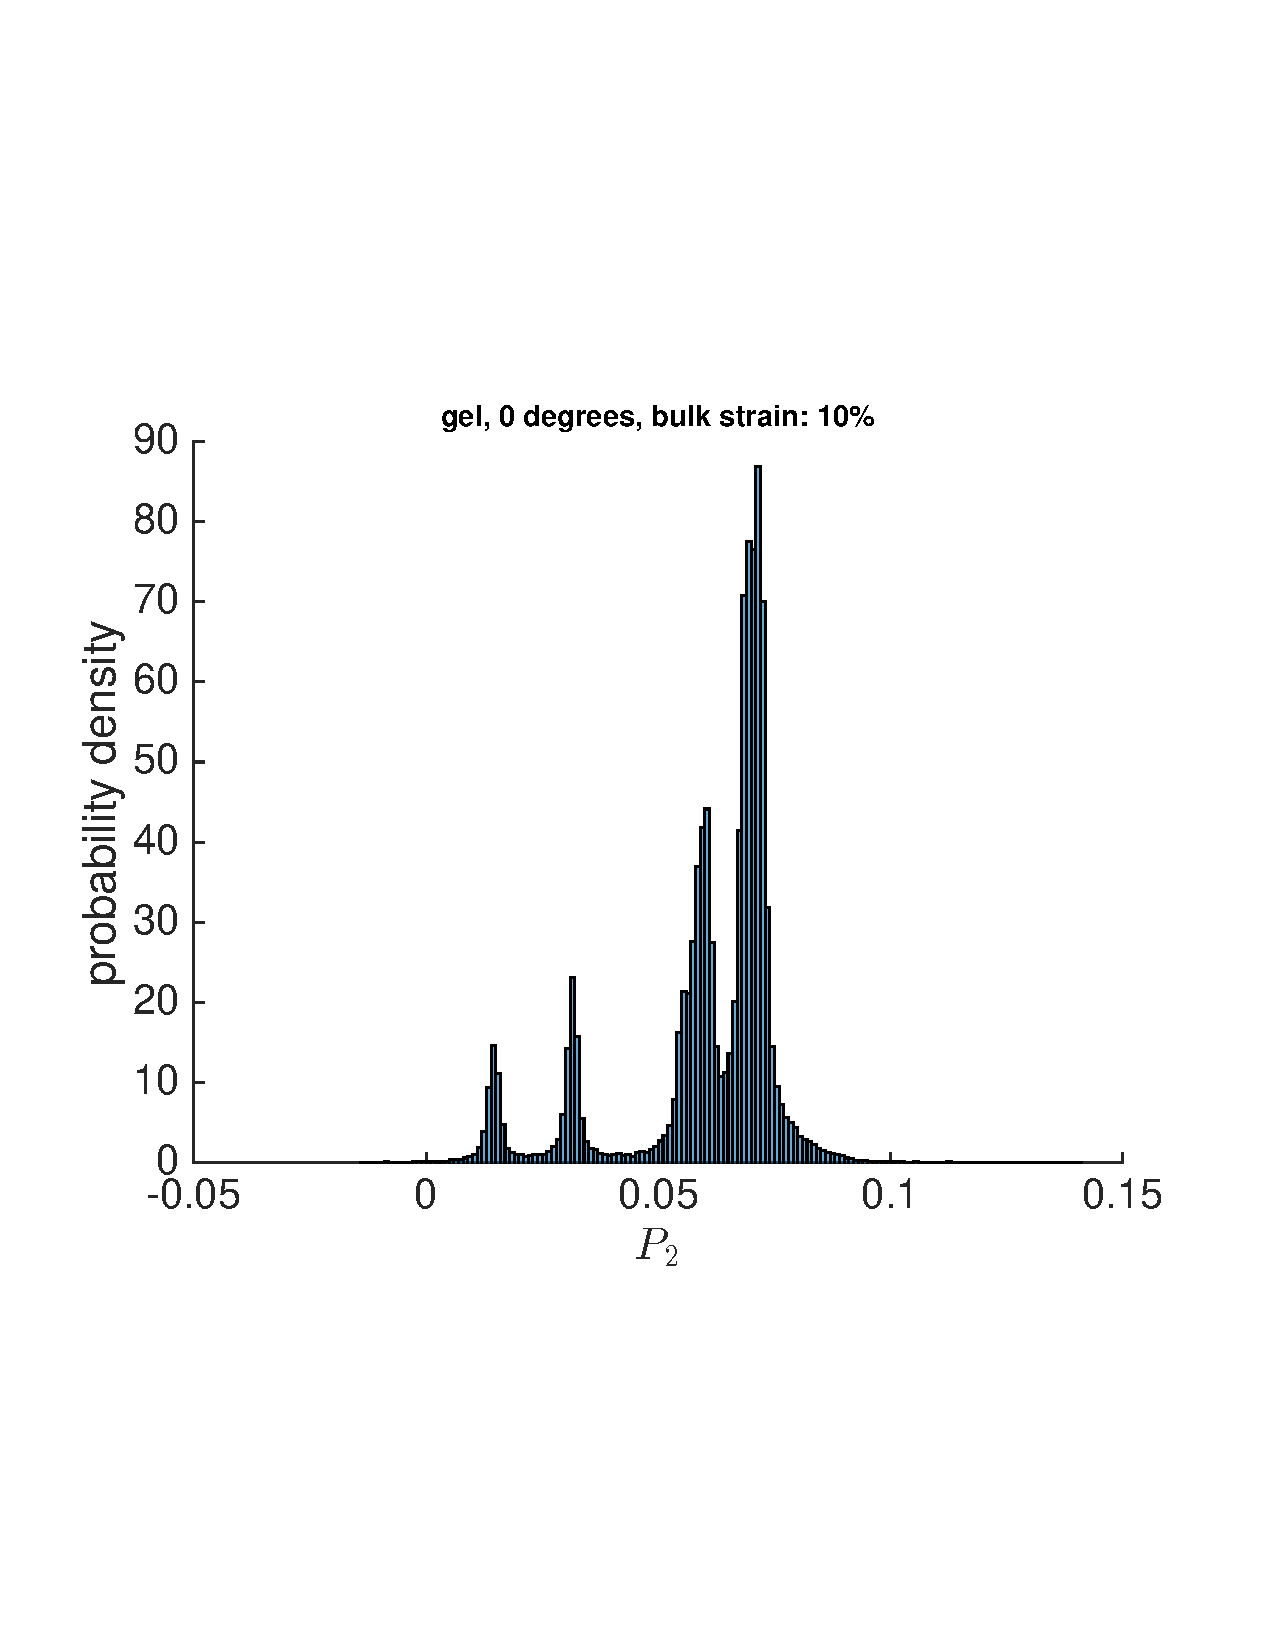
\includegraphics[height=4cm]{figure/rot0_FT50_128_1920_histo_gel_5.pdf} & 
%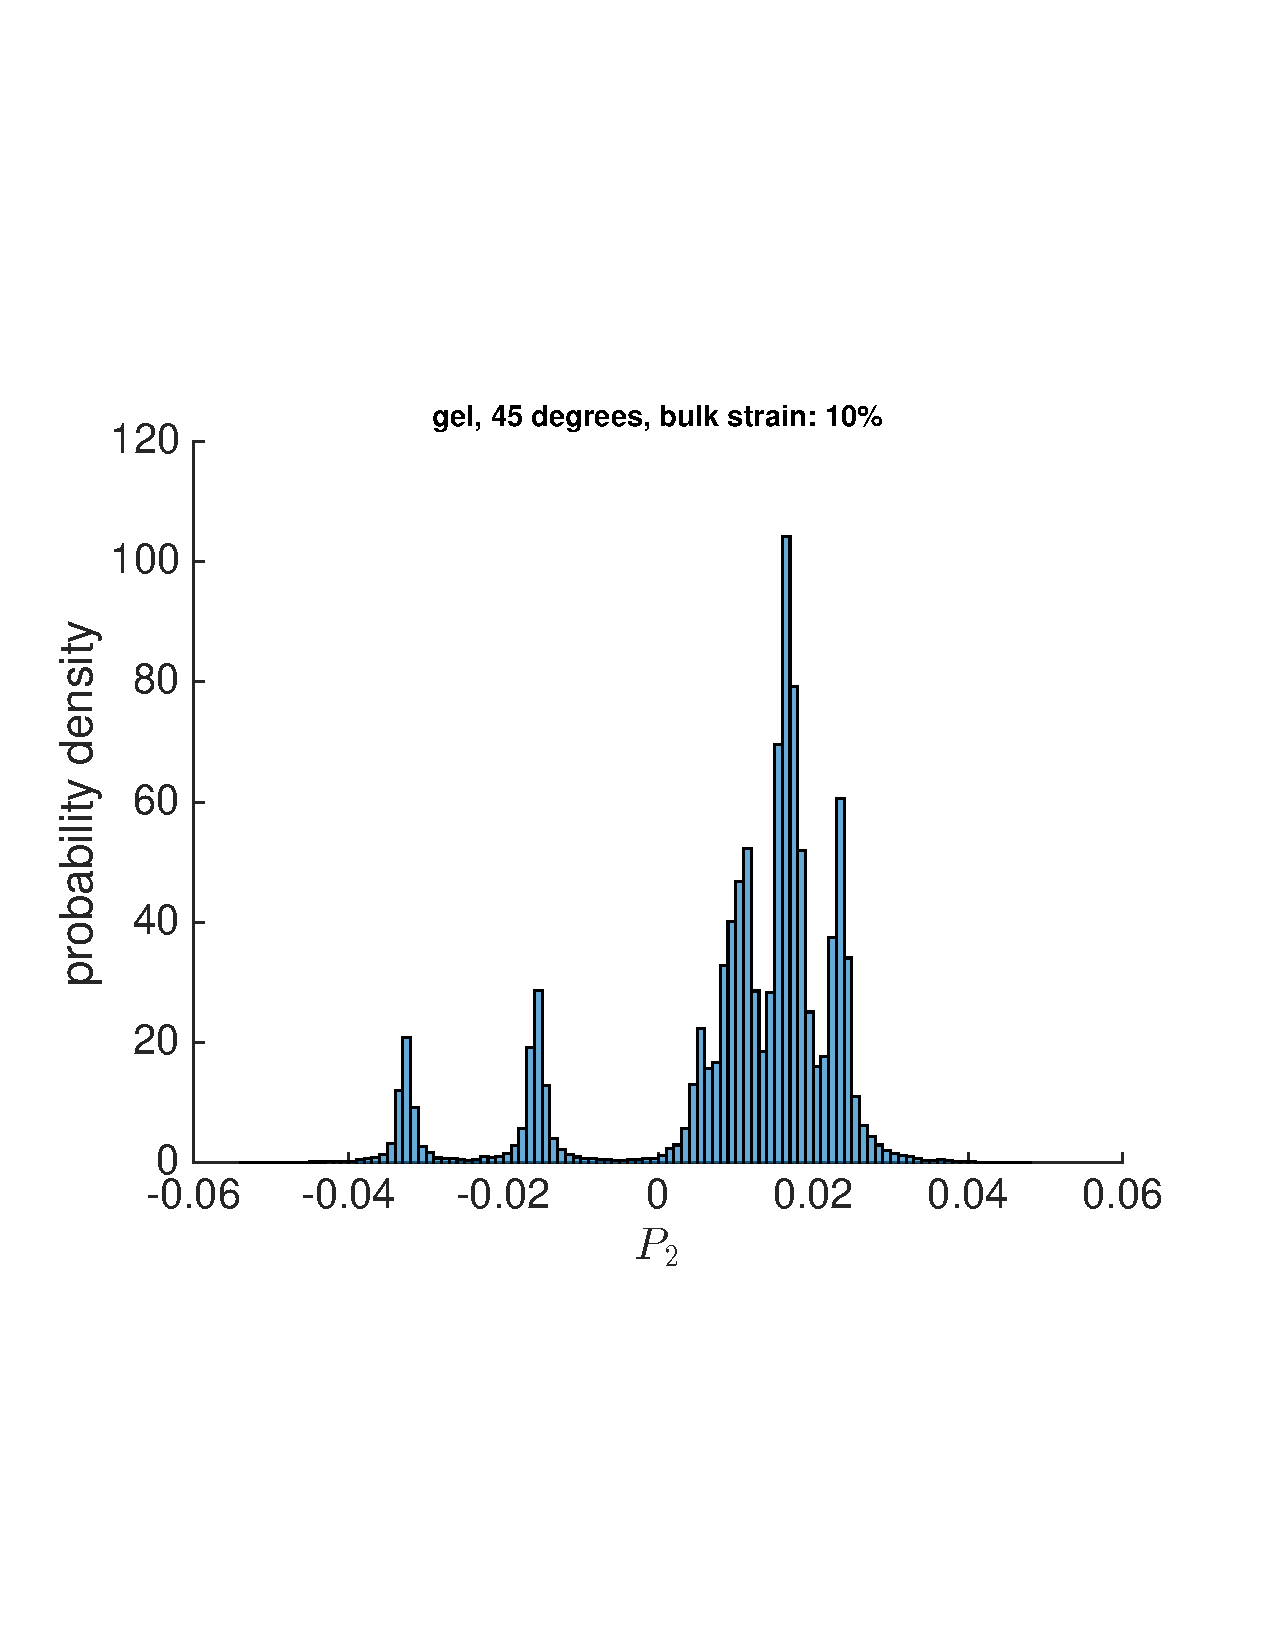
\includegraphics[height=4cm]{figure/rot45_FT50_128_1920_histo_gel_8.pdf} &
%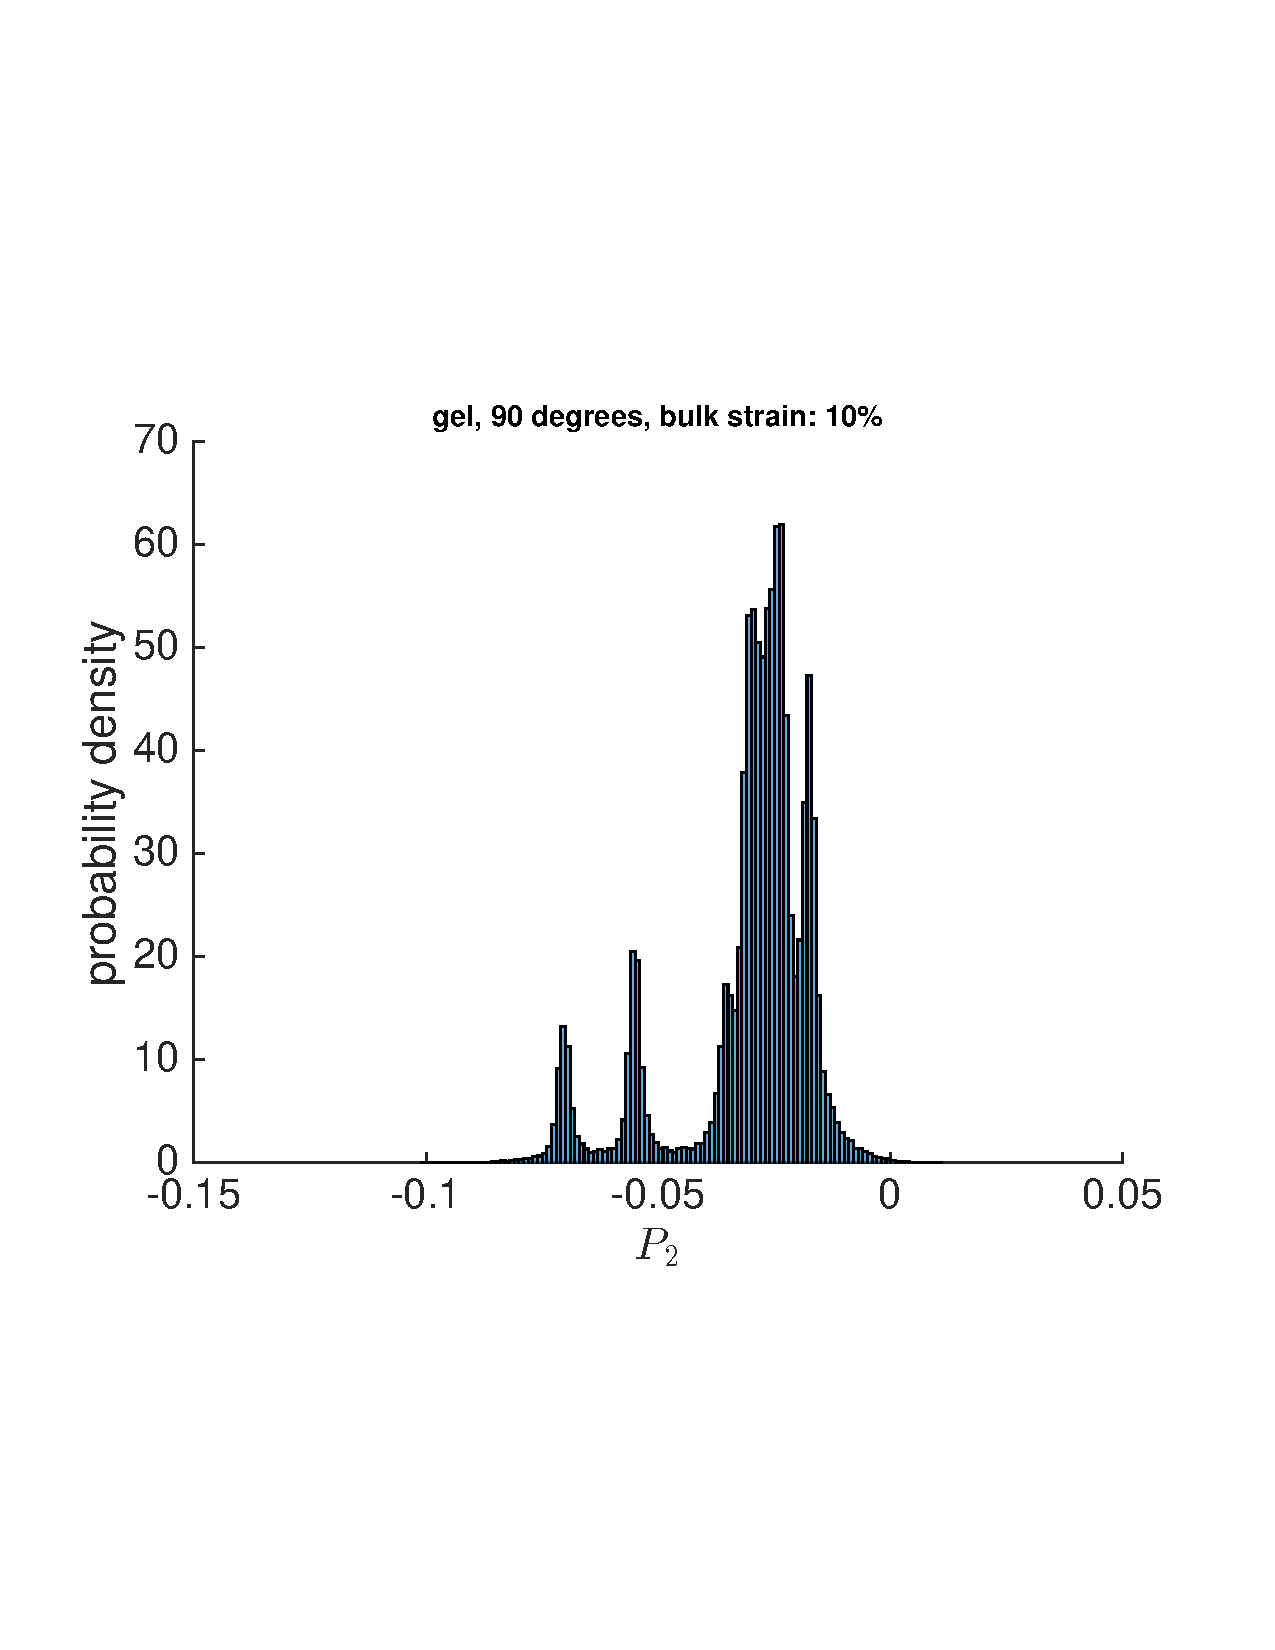
\includegraphics[height=4cm]{figure/rot90_FT_dspBC50_a30_128_1920_histo_gel_27.pdf} \\
%(a) & (b) & (c) \\ 
%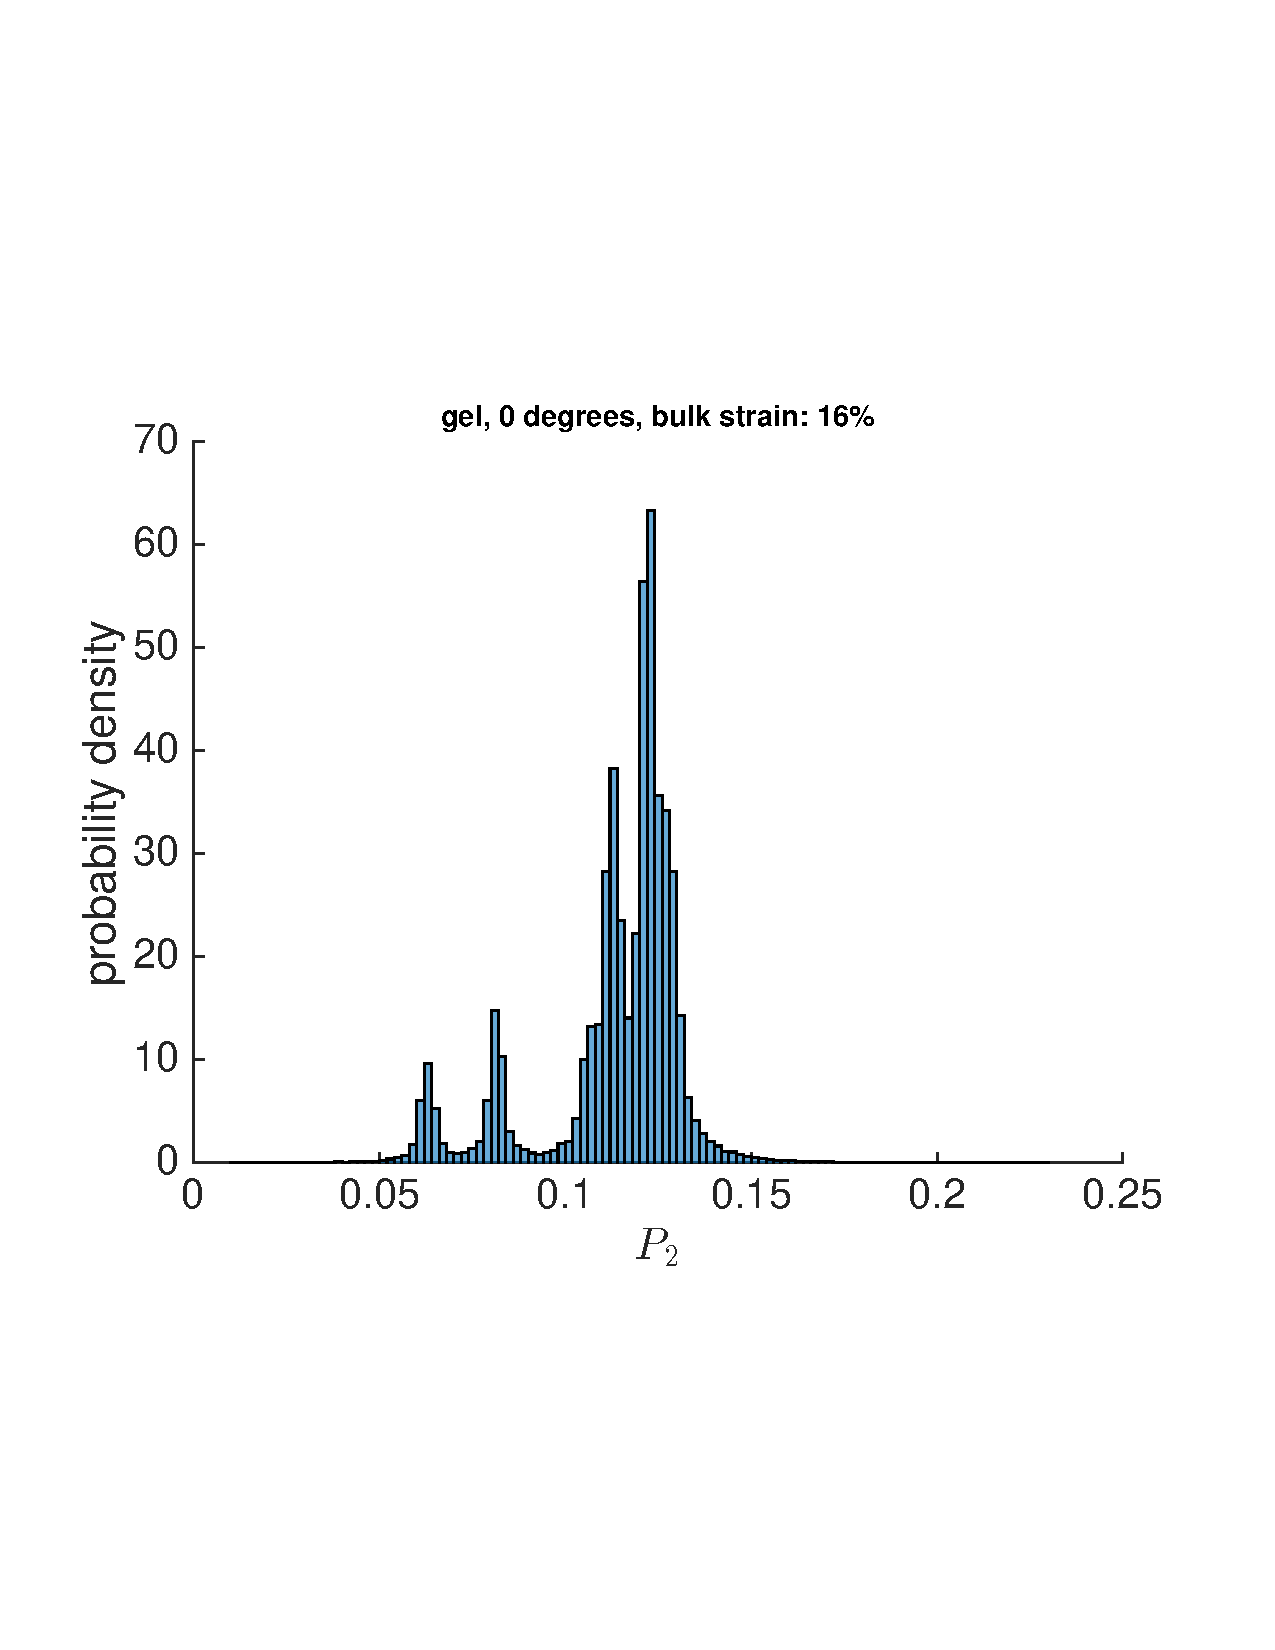
\includegraphics[height=4cm]{figure/rot0_FT50_128_1920_histo_gel_20.pdf} &
%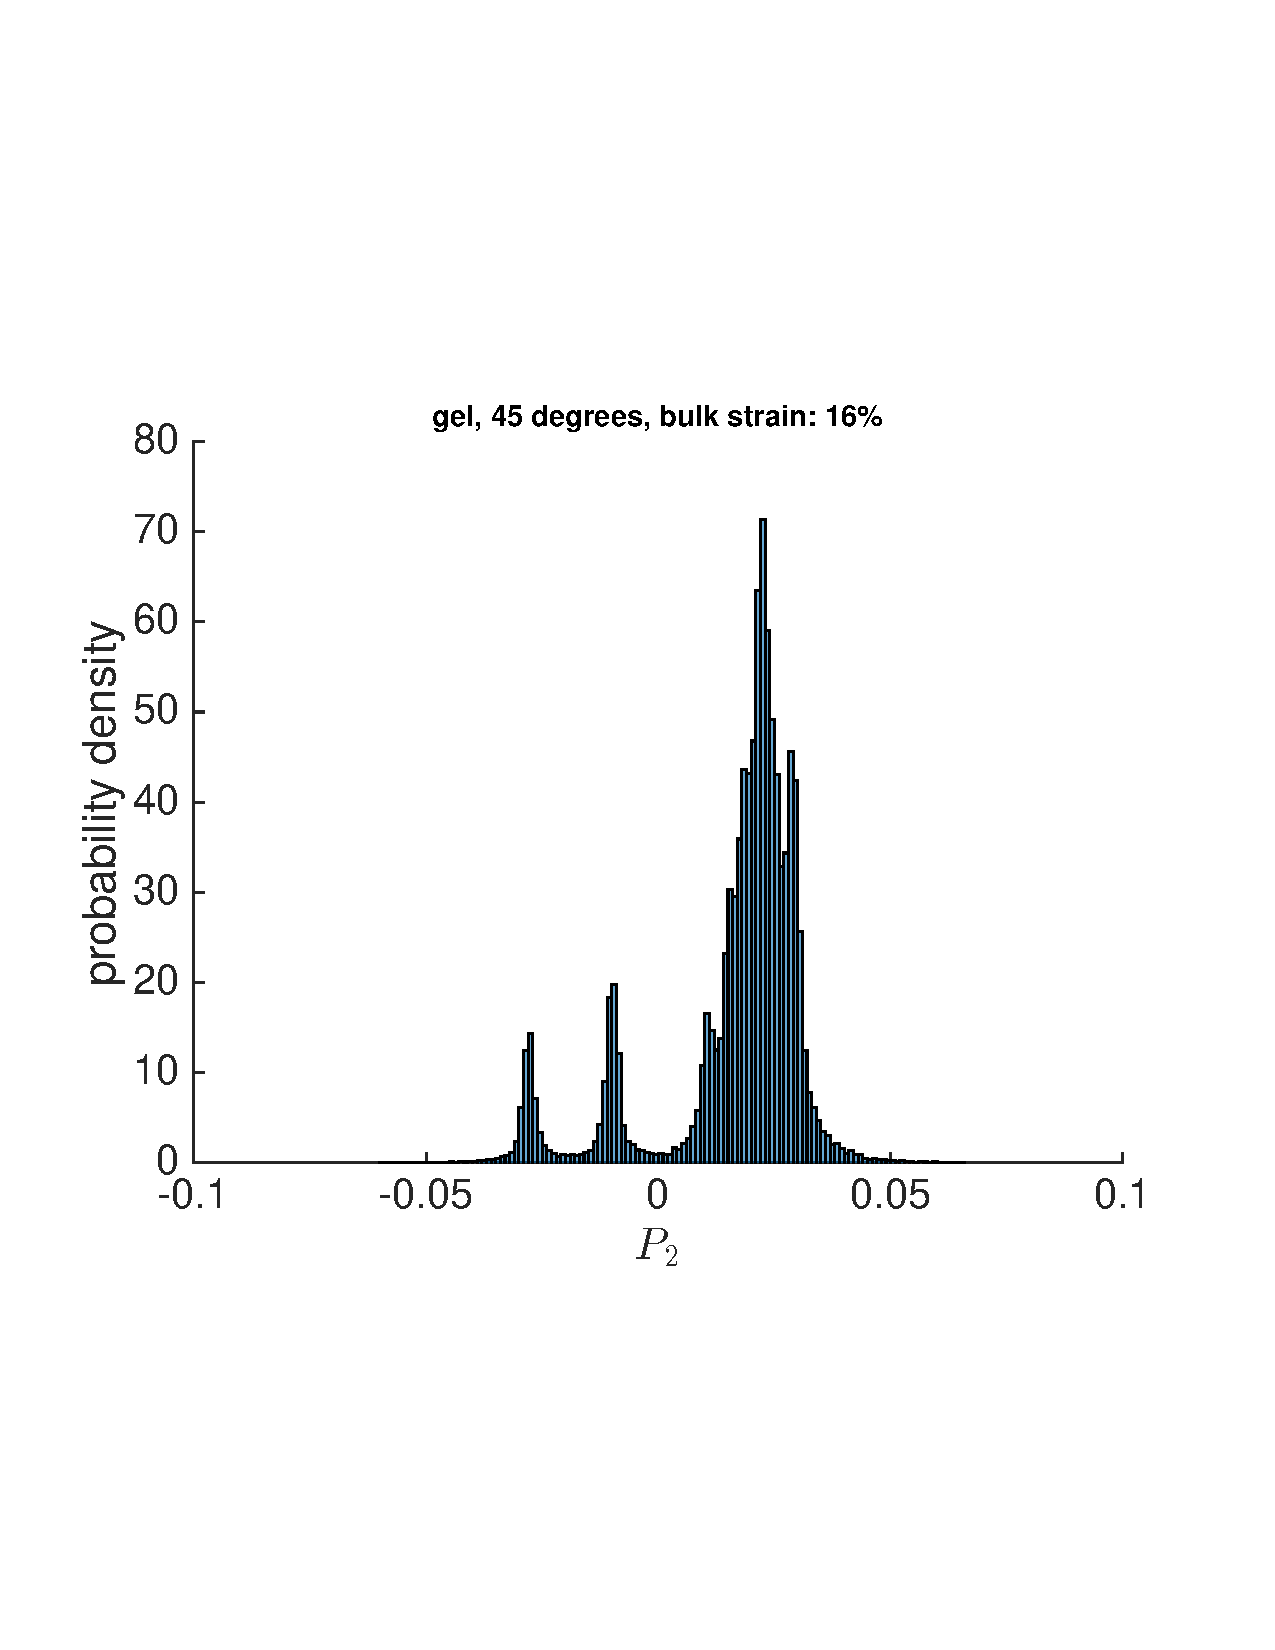
\includegraphics[height=4cm]{figure/rot45_FT50_128_1920_histo_gel_20.pdf} &
%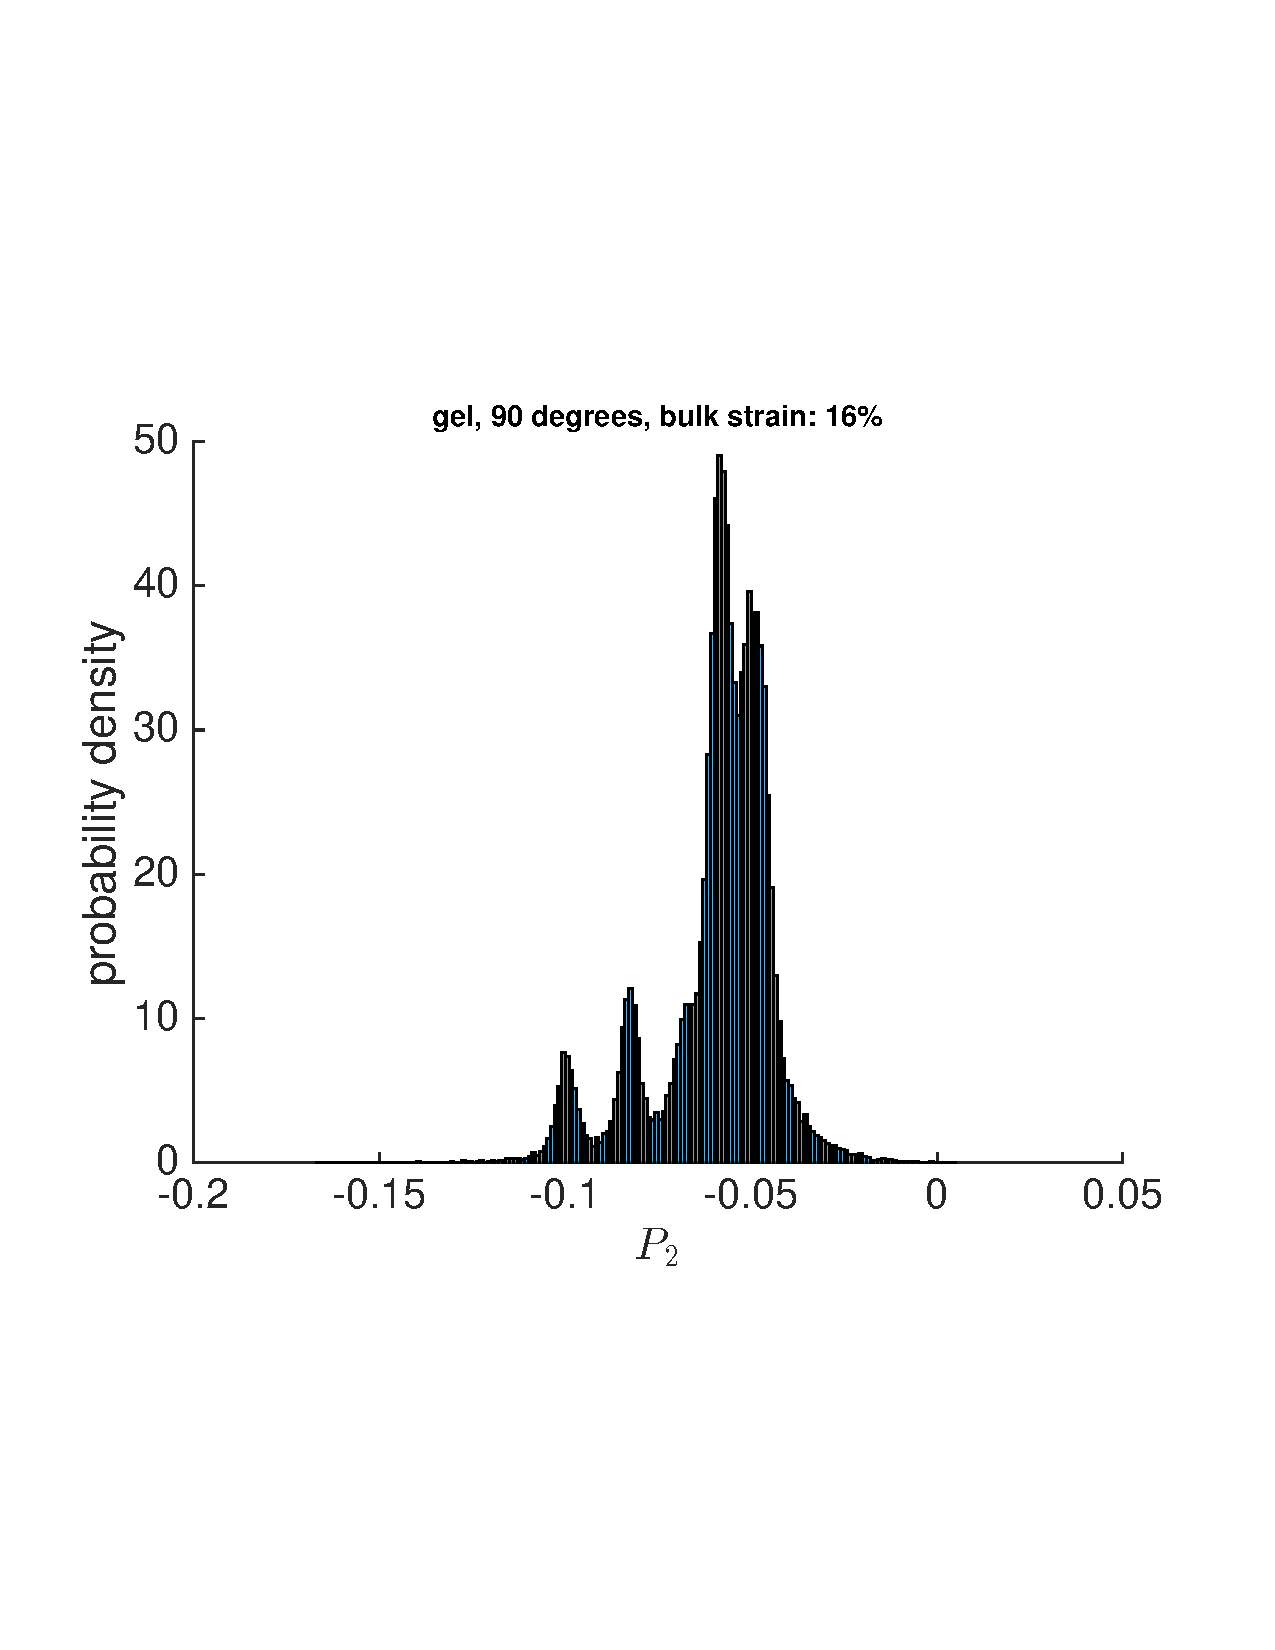
\includegraphics[height=4cm]{figure/rot90_FT_dspBC50_a30_128_1920_histo_gel_47.pdf} \\
%(d) & (e) & (f)
%\end{array}
%$
%\end{center}
%\caption{\label{fig:gel_P2} Distribution of $P_2$ in collagen gel for applied loads at 0 degrees (left column), 45 degrees (middle column), and 90 degrees (right column). The distributions for 10$\%$ (top row) and 16$\%$ (bottom row) bulk strain are shown. $P_2$ is calculated relative to the [1,0,0] axis, i.e., the axis along the direction of 0 degrees applied load.}
%\end{figure}
%%
%
%%
%\begin{figure}[ht]
%\begin{center}
%$
%\begin{array}{c}
%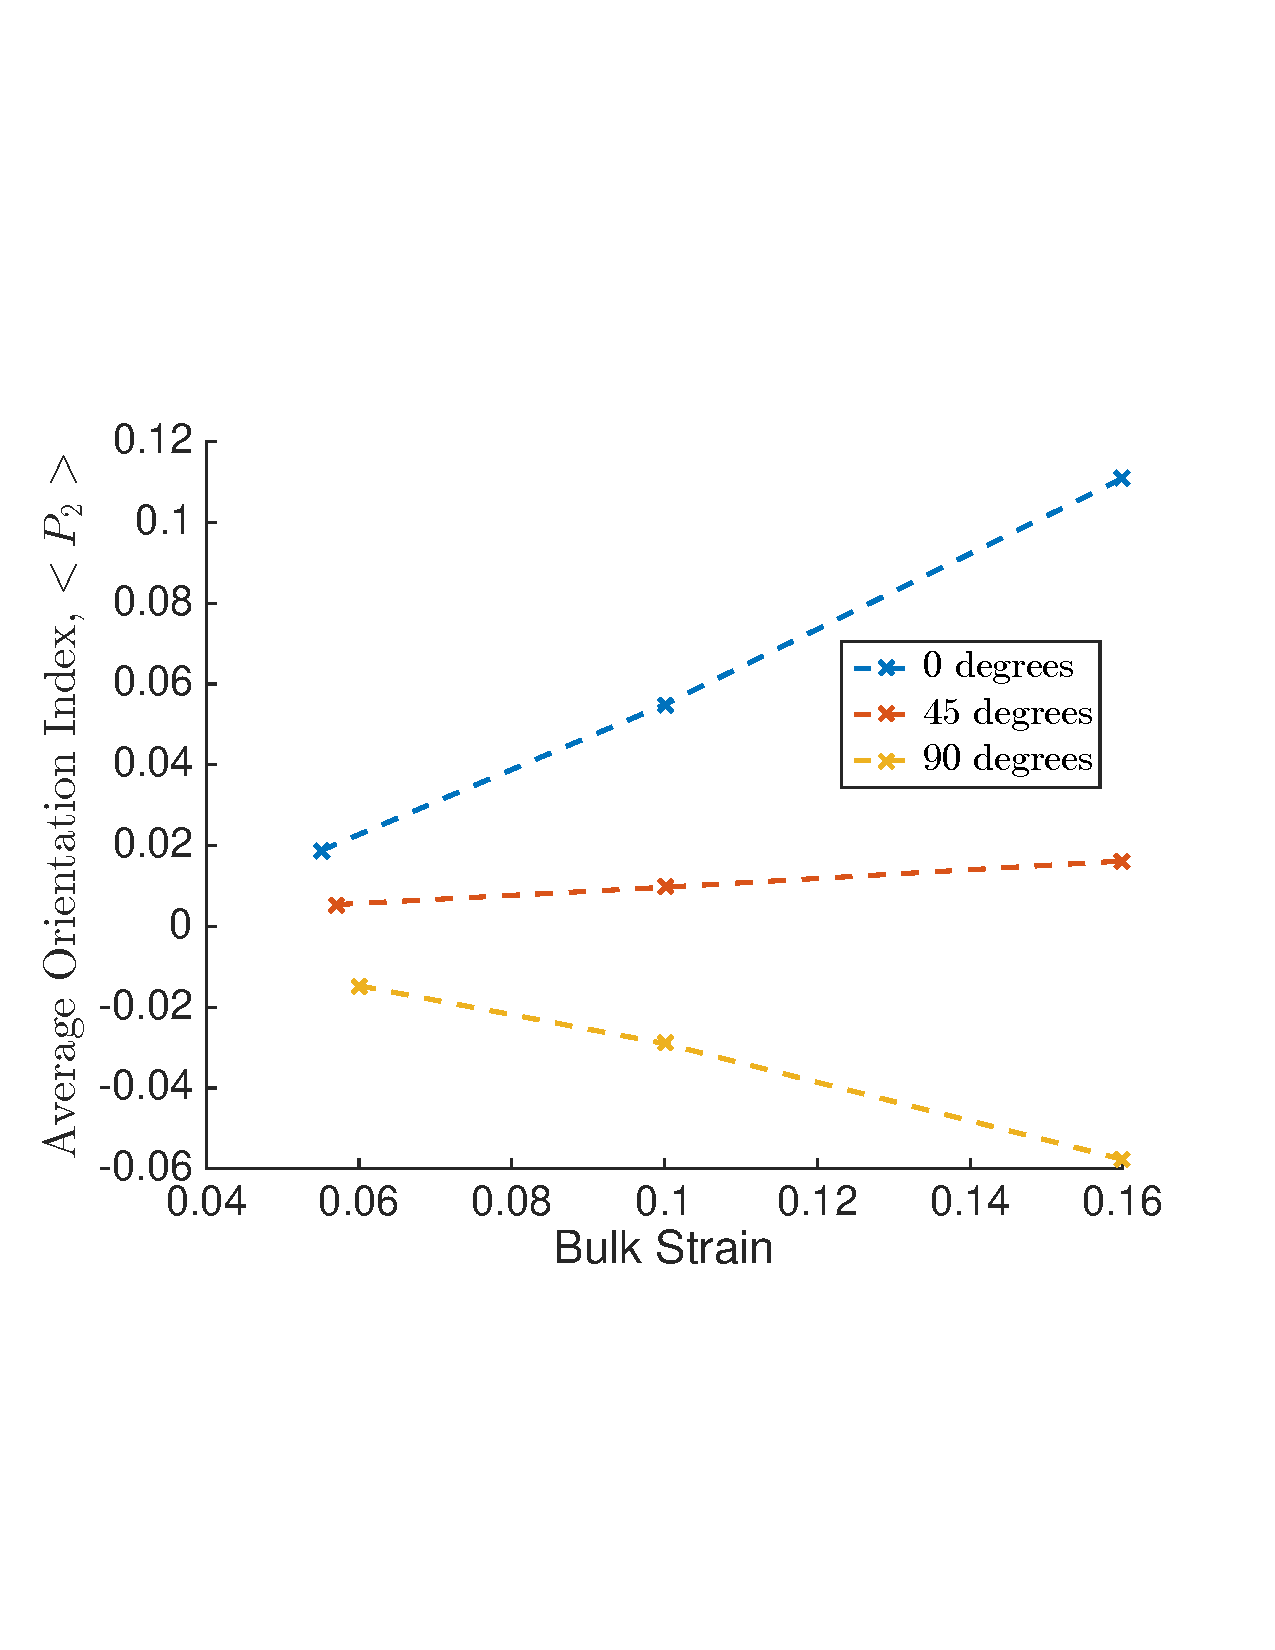
\includegraphics[height=6cm]{figure/avgP2.pdf} 
%\end{array}
%$
%\end{center}
%\caption{\label{fig:avg_P2} Average of $P_2$ in the gel for applied loads at 0, 45, and 90 degrees. $P_2$ is calculated relative to the [1,0,0] axis, i.e., the axis along the direction of 0 degrees applied load.}
%\end{figure}
%%
%%%%%%%%%%%%%%%%%%%%%%%%%%%%%%%%%%%%%%%%%%%%%%%%%%%%%%%%%%%%%%%%%%%%%%
\section{Conclusion}
\label{sec:conclusion}
In this paper we developed a multi-scale model of a neuron structure that is embedded in a collagen gel to examine the local strain response that arises when innervated collagenous tissue is deformed. The model presented in this work provides local strain information that is inaccessible by current experimental techniques, thereby serving as a computational microscope. Such local strain information was used to examine the embedded neuron structure's susceptibility to injury, which provides insights about the cause of pain when an innervated ligament is excessively loaded.

The embedded neuron geometry for this model was generated from confocal images to incorporate the complex structure of the neuron. The realistic representation of the embedded neuron structure enables us to extend our findings to actual physiological environments. The distribution of local strains that arise in the neuron structure were examined for different cell body stiffnesses in the neuron structure and loading configurations on the surrounding collagen gel. We showed that the local-strain distribution depends only weakly on the cell body stiffness, while varying significantly for different loading configurations. The strong dependence on loading configuration is a consequence of the anisotropic nature of the neuron, which has an axial stiffness that is one order greater that its transverse stiffness.

The spread in the strain distributions reflects the range of deformation that arises within the neuron structure due to its complex geometry; regions within the neuron structure experience different degrees of transverse and axial loading. We showed that transverse loading of the neuron gave rise to local-strain amplification, while axial loading gave rise to local strains in the neuron that are smaller than the applied load on the surrounding gel. Consequently, a larger average local-strain amplification corresponds to a larger degree of transverse loading in the neuron structure.

In this work, we considered loading along the 0, 45, and 90 degree axis, which are illustrated in Fig.\ \ref{fig:analysis_schematic}. As the loading angle varied from 0 to 90 degrees, the volume fraction of the neuron structure experiencing transverse loading increased, as reflected by the increasing average local-strain amplification. The neuron structure was loaded most uniformly at 45 degrees, as reflected by the relatively narrow spread of the strain distribution. At 0 and 90 degree loading, the neuron structure experiences the extremes of both nearly pure transverse and axial loading due to the existence of neurons that are nearly parallel to the 0 and 90 degree axes. Consequently, the spread in the distribution for 0 and 90 degree loading are wider.

The right tail of the distributions, which represent the maximum strain experienced in the neuron structure, was found to be the largest for the 90 degree loading case - 9.7$\%$ and 14$\%$ of the neuron structure experienced at least a three times local strain amplification for non painful and painful ligament loading, respectively. In contrast, 0.2$\%$ and 0$\%$ of the neuron structure experienced the same strain amplification for the 0 and 45 degree loading cases, respectively.

Overall, the 90 degree loading configuration was found to be most susceptible to neuronal injury because of the large average and long tail of its distribution. In the other cases, the strain distribution for 45 degree loading has a larger average while that for 0 degree loading has a longer tail. Therefore, whether the 0 or 45 degree loading configurations are more susceptible to neuronal injury depends on the strain threshold for damage on the neuron. For example, if the damage threshold is more than three times the applied strain, the 0 degree loading configuration is more susceptible to neuronal injury because of the longer tail in its distribution.

This study has provided initial insights about the local-strain amplifications that arise in the embedded neuron structure during deformation to the surrounding collagenous tissue. These findings support the hypothesis that embedded neurons can be damaged even when the surrounding collagenous tissue is moderately loaded. Additional insights on the cause of neuron damage during ligamentous matrix loading can be uncovered by extending this study to a larger number of embedded neurons. The technology presented in this work can be readily extended to such a system.

%%%%%%%%%%%%%%%%%%%%%%%%%%%%%%%%%%%%%%%%%%%%%%%%%%%%%%%%%%%%%%%%%%%%%%
%\begin{acknowledgment}
%\begin{enumerate}
%\item{NIH Grants}
%\item{Computing resources were provided by the Center for Computational Innovations at Rensselaer Polytechnic Institute \red{Will check specific wording on CCI website.}}
%\end{enumerate}
%\end{acknowledgment}

%%%%%%%%%%%%%%%%%%%%%%%%%%%%%%%%%%%%%%%%%%%%%%%%%%%%%%%%%%%%%%%%%%%%%%
% The bibliography is stored in an external database file
% in the BibTeX format (file_name.bib).  The bibliography is
% created by the following command and it will appear in this
% position in the document. You may, of course, create your
% own bibliography by using thebibliography environment as in
%
% \begin{thebibliography}{12}
% ...
% \bibitem{itemreference} D. E. Knudsen.
% {\em 1966 World Bnus Almanac.}
% {Permafrost Press, Novosibirsk.}
% ...
% \end{thebibliography}
\newpage
% Here's where you specify the bibliography style file.
% The full file name for the bibliography style file 
% used for an ASME paper is asmems4.bst.
%%\bibliographystyle{asmems4}
\bibliographystyle{tfcse}

% Here's where you specify the bibliography database file.
% The full file name of the bibliography database for this
% article is asme2e.bib. The name for your database is up
% to you.
\bibliography{references}


%%%%%%%%%%%%%%%%%%%%%%%%%%%%%%%%%%%%%%%%%%%%%%%%%%%%%%%%%%%%%%%%%%%%%%
\appendix
\section*{Appendix A: Derivation of $P_2$ from $\alpha$ and $\delta$ of the QPLI method}
\label{app:P2_derivation}

Consider a distribution of orientation $\theta$ for pixel $i$ as 
%
\begin{equation}
p_i(\theta) = q_i + r_i\cos^2(\theta - \alpha_i) \ \ \text{for} \ \ \theta \in (0,\pi),
\label{eq:distribution}
\end{equation}
%
where $\alpha_i$ is the alignment measured at pixel $i$ by the QPLI method and $q_i$ and $r_i$ are constants for the $i^{th}$ pixel. Applying the normalization 
%
\begin{equation}
\int_0^{\pi}p_i(\theta)d\theta = 1,
\end{equation}
%
a relationship between $q_i$ and $r_i$ is obtained:
%
\begin{equation}
\pi q_i + \frac{\pi}{2}r_i = 1.
\label{eq:q_relationship}
\end{equation}
%
Using the relationship in Eq.\ \eqref{eq:q_relationship}, Eq.\ \eqref{eq:distribution} can be rewritten as
%
\begin{equation}
p_i(\theta) = q_i + \frac{2}{\pi}(1-\pi q_i)\cos^2(\theta-\alpha_i)
\label{eq:distribution_q}
\end{equation}
%

The orientation tensor for each pixel can be written in terms of $p_i(\theta)$ as
%
\begin{eqnarray}
\pmb{A}^i = 
\begin{bmatrix}
\int_0^{\pi} p_i(\theta) \cos^2(\theta)d\theta & \int_0^{\pi} p_i(\theta) \sin(\theta) \cos(\theta)d\theta \\
\int_0^{\pi} p_i(\theta) \sin(\theta) \cos(\theta)d\theta & \int_0^{\pi} p_i(\theta) \sin^2(\theta)d\theta
\end{bmatrix} = 
%
\frac{1-\pi q_i}{4} 
\begin{bmatrix}
\cos(2 \alpha_i) & \sin(2 \alpha_i) \\
\sin(2\alpha_i) & - \cos(2\alpha_i)
\end{bmatrix},
\label{eq:Ai}
\end{eqnarray}
%
where the eigenvalues of $\pmb{A}^i$ are
\begin{equation}
\lambda_1 = \frac{1+\pi q_i}{4} \ \ \text{and} \ \ \lambda_2 = \frac{3-\pi q_i}{4}. 
\end{equation}
%
The retardation at each pixel, $\delta_i$, can be calculated from the eigenvalues by
%
\begin{equation}
\delta_i = |\lambda_2 - \lambda_1| = \frac{1-\pi q_i}{2}.
\label{eq:delta_i}
\end{equation}
%
From Eq.\ \eqref{eq:delta_i}, the constant $q_i$ can be written in terms of the retardation as
%
\begin{equation}
q_i = \frac{1}{\pi}(1-2\delta_i),
\end{equation}
%
and the distribution at pixel $i$ from Eq.\ \eqref{eq:distribution_q} can be rewritten as
%
\begin{equation}
p_i(\theta) = \frac{1-2\delta_i}{\pi} + \frac{4 \delta_i}{\pi}\cos^2(\theta-\alpha_i).
\label{eq:distribution_delta}
\end{equation}
%

The distribution of orientation $\theta$ for the entire image is simply the average over the distribution of each pixel
%
\begin{equation}
p(\theta) = \frac{1}{N} \sum_{i=1}^N p_i(\theta) = \frac{1}{N} \sum_{i=1}^N \left[ \frac{1-2\delta_i}{\pi} + \frac{4 \delta_i}{\pi}\cos^2(\theta-\alpha_i) \right],
\end{equation}
%
which is the equation presented in Eq.\ \eqref{eq:P2_experiment}.


\end{document}
